%\documentclass[12pt]{book}
%Paper saving
\documentclass[12pt,openany]{book}
%\documentclass[10pt,openany]{book}
%\documentclass[8pt,openany]{extbook}

\usepackage[T1]{fontenc}

% Footnotes should use symbols, not numbers.  Numbered footnotes are
% evil
\usepackage[perpage,symbol*]{footmisc}


\usepackage{enumerate}
\usepackage{ifpdf}
\usepackage{amsmath}
\usepackage[psamsfonts]{amsfonts}
\usepackage[psamsfonts]{amssymb}
\usepackage{amsthm}
\usepackage[pdftex]{graphicx}
%\usepackage{color}
%\usepackage{graphics}
\usepackage[headings]{fullpage}
\usepackage{url}
\usepackage{varioref}
%\usepackage{floatflt}
%\usepackage{wrapfig}
\usepackage{makeidx}
\usepackage[pdftex]{hyperref}
\usepackage[all]{hypcap}
\usepackage[alphabetic,msc-links]{amsrefs}
\usepackage[all]{xy}
\usepackage{nicefrac}
\usepackage{mathdots}
\usepackage{microtype}

\usepackage{tikz}
\usepackage{rotating}

% Times
%\usepackage{txfonts}
% Times, but symbol/cm/ams math fonts
\usepackage{mathptmx}
% But we do want helvetica for sans
\usepackage{helvet}


% useful
\newcommand{\ignore}[1]{}

% analysis/geometry stuff
\newcommand{\ann}{\operatorname{ann}}
\renewcommand{\Re}{\operatorname{Re}}
\renewcommand{\Im}{\operatorname{Im}}
\newcommand{\Orb}{\operatorname{Orb}}
\newcommand{\hol}{\operatorname{hol}}
\newcommand{\aut}{\operatorname{aut}}
\newcommand{\Aut}{\operatorname{Aut}}
\newcommand{\codim}{\operatorname{codim}}
\newcommand{\sing}{\operatorname{sing}}
\newcommand{\ord}{\operatorname{ord}}

% reals
\newcommand{\esssup}{\operatorname{ess~sup}}
\newcommand{\essran}{\operatorname{essran}}
\newcommand{\innprod}[2]{\langle #1 | #2 \rangle}
\newcommand{\linnprod}[2]{\langle #1 , #2 \rangle}
\newcommand{\supp}{\operatorname{supp}}
\newcommand{\Nul}{\operatorname{Nul}}
\newcommand{\Ran}{\operatorname{Ran}}
\newcommand{\sabs}[1]{\lvert {#1} \rvert}
\newcommand{\snorm}[1]{\lVert {#1} \rVert}
\newcommand{\abs}[1]{\left\lvert {#1} \right\rvert}
\newcommand{\norm}[1]{\left\lVert {#1} \right\rVert}
\newcommand{\smnorm}[1]{\lVert {#1} \rVert}

% sets (some)
\newcommand{\C}{{\mathbb{C}}}
\newcommand{\R}{{\mathbb{R}}}
\newcommand{\Z}{{\mathbb{Z}}}
\newcommand{\N}{{\mathbb{N}}}
\newcommand{\Q}{{\mathbb{Q}}}
\newcommand{\D}{{\mathbb{D}}}
\newcommand{\F}{{\mathbb{F}}}

% consistent
\newcommand{\bB}{{\mathbb{B}}}
\newcommand{\bC}{{\mathbb{C}}}
\newcommand{\bR}{{\mathbb{R}}}
\newcommand{\bZ}{{\mathbb{Z}}}
\newcommand{\bN}{{\mathbb{N}}}
\newcommand{\bQ}{{\mathbb{Q}}}
\newcommand{\bD}{{\mathbb{D}}}
\newcommand{\bF}{{\mathbb{F}}}
\newcommand{\bH}{{\mathbb{H}}}
\newcommand{\bO}{{\mathbb{O}}}
\newcommand{\bP}{{\mathbb{P}}}
\newcommand{\bK}{{\mathbb{K}}}
\newcommand{\bV}{{\mathbb{V}}}
\newcommand{\CP}{{\mathbb{CP}}}
\newcommand{\RP}{{\mathbb{RP}}}
\newcommand{\HP}{{\mathbb{HP}}}
\newcommand{\OP}{{\mathbb{OP}}}
\newcommand{\sA}{{\mathcal{A}}}
\newcommand{\sB}{{\mathcal{B}}}
\newcommand{\sC}{{\mathcal{C}}}
\newcommand{\sF}{{\mathcal{F}}}
\newcommand{\sG}{{\mathcal{G}}}
\newcommand{\sH}{{\mathcal{H}}}
\newcommand{\sM}{{\mathcal{M}}}
\newcommand{\sO}{{\mathcal{O}}}
\newcommand{\sP}{{\mathcal{P}}}
\newcommand{\sQ}{{\mathcal{Q}}}
\newcommand{\sR}{{\mathcal{R}}}
\newcommand{\sS}{{\mathcal{S}}}
\newcommand{\sI}{{\mathcal{I}}}
\newcommand{\sL}{{\mathcal{L}}}
\newcommand{\sK}{{\mathcal{K}}}
\newcommand{\sU}{{\mathcal{U}}}
\newcommand{\sV}{{\mathcal{V}}}
\newcommand{\sX}{{\mathcal{X}}}
\newcommand{\sY}{{\mathcal{Y}}}
\newcommand{\sZ}{{\mathcal{Z}}}
\newcommand{\fS}{{\mathfrak{S}}}

\newcommand{\interior}{\operatorname{int}}

% Topo stuff
\newcommand{\id}{\textit{id}}
\newcommand{\im}{\operatorname{im}}
\newcommand{\rank}{\operatorname{rank}}
\newcommand{\Tor}{\operatorname{Tor}}
\newcommand{\Torsion}{\operatorname{Torsion}}
\newcommand{\Ext}{\operatorname{Ext}}
\newcommand{\Hom}{\operatorname{Hom}}

%extra thingies
\newcommand{\mapsfrom}{\ensuremath{\text{\reflectbox{$\mapsto$}}}}
\newcommand{\from}{\ensuremath{\leftarrow}}
\newcommand{\dhat}[1]{\hat{\hat{#1}}}

% San Serif fonts
%\renewcommand{\familydefault}{\sfdefault}

% To allow skrinking to 5.5 x 8.5 inches without whitespaces
% Make sure to rerun makeindex as well
% Useful for printing on lilu.com and saving on paper
%\addtolength{\textheight}{2.13in}
%\addtolength{\paperheight}{2.13in}

\hypersetup{
    %colorlinks,
    pdfborderstyle={/S/U/W 1},
    %citecolor=black,
    %filecolor=black,
    %linkcolor=black,
    %urlcolor=black,
    pdftitle={Hermitian Forms Meet Several Complex Variables},
    pdfsubject={Several Complex Variables},
    pdfkeywords={several complex variables, Hermitian forms, complex analysis},
    pdfauthor={Jiri Lebl}
}

% Set up our index
\makeindex

% Very simple indexing
\newcommand{\myindex}[1]{#1\index{#1}}

% define this to be empty to kill notes
\newcommand{\sectionnotes}[1]{\noindent \emph{Note: #1} \medskip \par}

% Define this to be empty to not skip page before the sections to
% save some paper
%\newcommand{\sectionnewpage}{\clearpage}
\newcommand{\sectionnewpage}{}

\author{Ji\v{r}\'i Lebl}

\title{Hermitian Forms Meet Several Complex Variables}

% Don't include subsections
\setcounter{tocdepth}{1}

\theoremstyle{plain}
\newtheorem{thm}{Theorem}[section]
\newtheorem{lemma}[thm]{Lemma}
\newtheorem{prop}[thm]{Proposition}
\newtheorem{cor}[thm]{Corollary}

\theoremstyle{remark}
\newtheorem{remark}[thm]{Remark}

\theoremstyle{definition}
\newtheorem{defn}[thm]{Definition}

\newtheoremstyle{exercise}% name
  {}% Space above
  {}% Space below
  {\itshape}% Body font
  {}% Indent amount 1
  {\bfseries \itshape}% Theorem head font
  {:}% Punctuation after theorem head
  {.5em}% Space after theorem head 2
  {}% Theorem head spec (can be left empty, meaning "normal")


\theoremstyle{exercise}
\newtheorem{exercise}{Exercise}[section]

\newtheoremstyle{example}% name
  {}% Space above
  {}% Space below
  {}% Body font
  {}% Indent amount 1
  {\bfseries}% Theorem head font
  {:}% Punctuation after theorem head
  {.5em}% Space after theorem head 2
  {}% Theorem head spec (can be left empty, meaning "normal")

\theoremstyle{example}
\newtheorem{example}[thm]{Example}

% referencing
\newcommand{\figureref}[1]{\hyperref[#1]{Figure~\ref*{#1}}}
\newcommand{\tableref}[1]{\hyperref[#1]{Table~\ref*{#1}}}
\newcommand{\chapterref}[1]{\hyperref[#1]{chapter~\ref*{#1}}}
\newcommand{\Chapterref}[1]{\hyperref[#1]{Chapter~\ref*{#1}}}
\newcommand{\sectionref}[1]{\hyperref[#1]{section~\ref*{#1}}}
\newcommand{\exerciseref}[1]{\hyperref[#1]{Exercise~\ref*{#1}}}
\newcommand{\exampleref}[1]{\hyperref[#1]{Example~\ref*{#1}}}
\newcommand{\thmref}[1]{\hyperref[#1]{Theorem~\ref*{#1}}}
\newcommand{\propref}[1]{\hyperref[#1]{Proposition~\ref*{#1}}}
\newcommand{\lemmaref}[1]{\hyperref[#1]{Lemma~\ref*{#1}}}
\newcommand{\corref}[1]{\hyperref[#1]{Corollary~\ref*{#1}}}
\newcommand{\defnref}[1]{\hyperref[#1]{Definition~\ref*{#1}}}

\begin{document}

\ifpdf
  \pdfbookmark{Title Page}{title}
\fi
\newlength{\centeroffset}
\setlength{\centeroffset}{-0.5\oddsidemargin}
\addtolength{\centeroffset}{0.5\evensidemargin}
%\addtolength{\textwidth}{-\centeroffset}
\thispagestyle{empty}
\vspace*{\stretch{1}}
\noindent\hspace*{\centeroffset}\makebox[0pt][l]{\begin{minipage}{\textwidth}
\flushright
{\Huge\bfseries \sffamily Hermitian Forms Meet Several Complex Variables }
\noindent\rule[-1ex]{\textwidth}{5pt}\\[2.5ex]
\hfill\emph{\Large \sffamily Minicourse on CR Geometry Using Hermitian Forms}
\end{minipage}}

\vspace{\stretch{1}}
\noindent\hspace*{\centeroffset}\makebox[0pt][l]{\begin{minipage}{\textwidth}
\flushright
{\bfseries 
by Ji{\v r}\'i Lebl\\[3ex]} 
\today
\end{minipage}}

%\addtolength{\textwidth}{\centeroffset}
\vspace{\stretch{2}}


\pagebreak

\vspace*{\fill}

%\begin{small} 
\noindent
Typeset in \LaTeX.

\bigskip

\noindent
Copyright \copyright 2011 Ji{\v r}\'i Lebl

\bigskip

%\begin{floatingfigure}{1.4in}
%\vspace{-0.05in}
\noindent
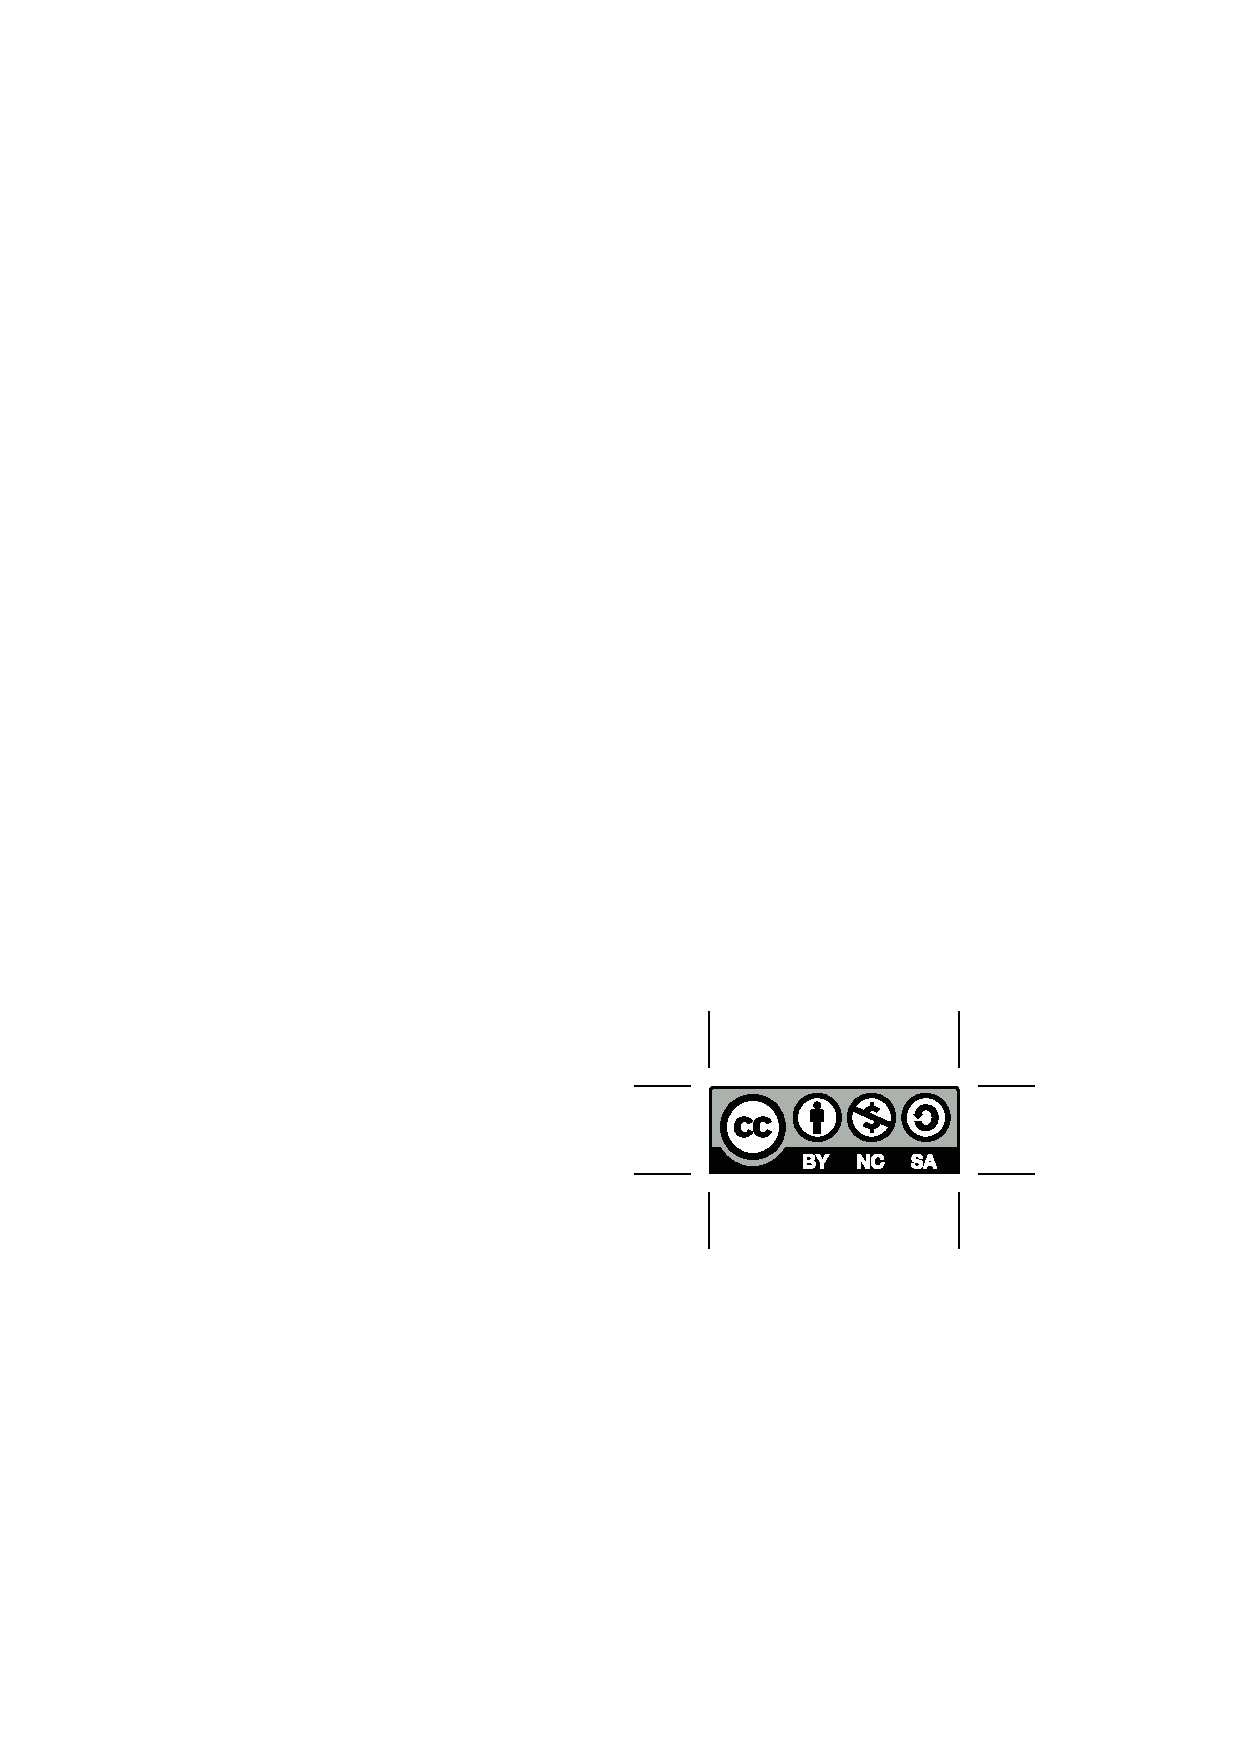
\includegraphics[width=1.38in]{license}
%\end{floatingfigure}

\bigskip

\noindent
This work is licensed under the Creative Commons
Attribution-Non\-commercial-Share Alike 3.0 United States License. To view a
copy of this license, visit
\url{http://creativecommons.org/licenses/by-nc-sa/3.0/us/} or send a letter to
Creative Commons, 171 Second Street, Suite 300, San Francisco, California,
94105, USA.
%\end{small}

\bigskip

\noindent
You can use, print, duplicate, share these notes as much as you want.  You can
base your own notes on these and reuse parts if you keep the license the
same.  If you plan to use these commercially (sell them for more than just
duplicating cost), then you need to contact me and we will work something out.
If you are printing a course pack for your students, then it is fine if the 
duplication service is charging a fee for printing and selling the printed
copy.  I consider that duplicating cost.

\bigskip

\noindent
During the writing of these notes, 
the author was in part supported by NSF grant DMS-0900885.

\bigskip

\noindent
See \url{http://www.jirka.org/scv-mini/} for more information
(including contact information).


% For large print do this
%\large

\microtypesetup{protrusion=false}
\tableofcontents
\microtypesetup{protrusion=true}

\newpage

%%%%%%%%%%%%%%%%%%%%%%%%%%%%%%%%%%%%%%%%%%%%%%%%%%%%%%%%%%%%%%%%%%%%%%%%%%%%%%
%%%%%%%%%%%%%%%%%%%%%%%%%%%%%%%%%%%%%%%%%%%%%%%%%%%%%%%%%%%%%%%%%%%%%%%%%%%%%%
%%%%%%%%%%%%%%%%%%%%%%%%%%%%%%%%%%%%%%%%%%%%%%%%%%%%%%%%%%%%%%%%%%%%%%%%%%%%%%

\chapter*{Introduction}
\addcontentsline{toc}{chapter}{Introduction}
\markboth{INTRODUCTION}{INTRODUCTION}

%%%%%%%%%%%%%%%%%%%%%%%%%%%%%%%%%%%%%%%%%%%%%%%%%%%%%%%%%%%%%%%%%%%%%%%%%%%%%%

\section{Notes about these notes}

These were the lecture notes for a graduate Math 595 half-semester
mini-course at \href{http://www.math.uiuc.edu/}{University of Illinois at
Urbana-Champaign} on Several Complex Variables given in Spring 2010.
Prerequisites are one variable complex analysis, linear algebra, real
analysis and basic functional analysis.  The notes are not meant as a
polished finished product.  I hope they are usable as a quick and dirty
introduction to the subject.  Due to time constraints much is missing.  For
example, the Levi form, nor pseudoconvexity is not mentioned.  The focus is
on geometry using Hermitian forms rather than analysis.

The notes are also not completely self contained.  There are many proofs
in the beginning sections about complex geometry that are left
out due to lack of time in the course.  Some material from the course did not
make it into these notes and vice-versa.

There are most likely many typos and minor errors throughout (hopefully no
major ones), so be wary.  Do email me any errors you find so that they get
fixed.
See \url{http://www.jirka.org/scv-mini/} for more info.

The structure of the course is the following.

\begin{enumerate}
\item \emph{\hyperref[cav:chapter]{Complex Analytic Varieties.}}  This chapter covers the very
basics of complex geometry and holomorphic functions of several variables.
\item \emph{\hyperref[cr:chapter]{CR Geometry.}}  We solve some basic problems in CR geometry using
Hermitian forms.  The chapter begins with the inequivalence of the ball and
polydisc in $\C^2$ for motivation.
\item \emph{\hyperref[proper:chapter]{Proper Maps of Balls.}}  A very natural place where Hermitian
forms arise are proper maps of balls and hyperquadrics.  We cover this topic
in this chapter.
\end{enumerate}

I would like to acknowledge my SCV minicourse class at UIUC for any comments
during the class, and especially Dusty Grundmeier.  I would also like to
acknowledge Montgomery Taylor and Jianou Zhang for reading through and finding errors.

%%%%%%%%%%%%%%%%%%%%%%%%%%%%%%%%%%%%%%%%%%%%%%%%%%%%%%%%%%%%%%%%%%%%%%%%%%%%%%
%%%%%%%%%%%%%%%%%%%%%%%%%%%%%%%%%%%%%%%%%%%%%%%%%%%%%%%%%%%%%%%%%%%%%%%%%%%%%%
%%%%%%%%%%%%%%%%%%%%%%%%%%%%%%%%%%%%%%%%%%%%%%%%%%%%%%%%%%%%%%%%%%%%%%%%%%%%%%

\chapter{Complex Analytic Varieties} \label{cav:chapter}

%%%%%%%%%%%%%%%%%%%%%%%%%%%%%%%%%%%%%%%%%%%%%%%%%%%%%%%%%%%%%%%%%%%%%%%%%%%%%%

\section{Holomorphic functions} \label{sec:holfunc}

Let $\C^n$ denote the complex Euclidean space.  We denote
by $z = (z_1,\ldots,z_n)$ the coordinates of $\C^n$.
Let $x =
(x_1,\ldots,x_n)$ and $y = (y_1,\ldots,y_n)$ denote the coordinates in
$\R^n$.
We can 
identify $\C^n$ with $\R^n \times \R^n = \R^{2n}$ by letting
$z = x+iy$.
Just as in one complex variable we write $\bar{z} = x-iy$.
We call $z$ the \emph{\myindex{holomorphic coordinates}}
and $\bar{z}$ the \emph{\myindex{antiholomorphic coordinates}}.

\begin{defn}
For $\rho = (\rho_1,\ldots,\rho_n)$ where $\rho_j > 0$ and $a \in \C^n$
define
a \emph{\myindex{polydisc}}
\begin{equation}
\Delta_\rho(a)  \overset{\text{def}}{=} \{ z \in \C^n : \abs{z_j - a_j} < \rho_j \} .
\end{equation}
We call $a$ the
\emph{center}\index{center of a polydisc}
and $\rho$ the
\emph{polyradius}\index{polyradius of a polydisc}
or simply the
\emph{radius}\index{radius of a polydisc}
of the polydisc $\Delta_\rho(a)$.
\end{defn}

At this point it will be useful to recall the
\emph{\myindex{Euclidean inner product}}
\begin{equation}
\linnprod{z}{w} = z \cdot \bar{w}
=
z_1 \bar{w}_1 + \cdots +
z_n \bar{w}_n .
\end{equation}
Using the inner product we obtain the standard
\emph{\myindex{Euclidean norm}}
\begin{equation}
\norm{z}  \overset{\text{def}}{=} \sqrt{\linnprod{z}{z}}
=
\sqrt{\abs{z_1}^2 + \cdots +
\abs{z_n}^2} .
\end{equation}

As in complex analysis in one variable we define the formal operators
\begin{align}
\frac{\partial}{\partial z_j} &  \overset{\text{def}}{=}
\frac{1}{2} \left(
\frac{\partial}{\partial x_j} - i \frac{\partial}{\partial y^j}
\right) ,
\\
\frac{\partial}{\partial \bar{z}_j} &  \overset{\text{def}}{=}
\frac{1}{2} \left(
\frac{\partial}{\partial x_j} + i \frac{\partial}{\partial y_j}
\right) .
\end{align}

\begin{defn}
Let $U \subset
\C^n$ be an open set, and let $f \colon U \to \C$ be a continuously
differentiable function.  We say that $f$ is \emph{\myindex{holomorphic}}
if it satisfies the Cauchy-Riemann equations
\begin{equation}
\frac{\partial f}{\partial \bar{z}_j}  = 0 \qquad \text{for $j=1,\ldots,n$}.
\end{equation}
\end{defn}

In other words, $f$ is holomorphic if it is holomorphic in each variable
separately as a function of one variable.  Suppose that $f$ is holomorphic
in some polydisc $\Delta = \Delta_{\rho}(a) = \Delta_1 \times \cdots \times \Delta_n$
centered at $a$, where $\Delta_j \subset \C$ is a disc.
Suppose that $f$ is continuous
on the closure $\overline{\Delta}$.
We can apply the Cauchy formula:
\begin{equation}
f(z) =
\frac{1}{2\pi i}
\int_{\partial \Delta_1}
\frac{f(\zeta_1,z_2,\ldots,z_n)}{\zeta_1-z_1}
d \zeta_1 .
\end{equation}
We apply the formula $n-1$ more times and write the integral
as a single integral.  The operation requires the Fubini theorem, which applies
as $f$ is continuous on the closed polydisc.  We obtain the
Cauchy integral formula in several variables.

\begin{thm}[Cauchy integral formula]
\index{Cauchy integral formula in several variables}
Let $\Delta$ be a polydisc centered at $a \in \C^n$.  Suppose
that $f \colon \overline{\Delta} \to \C$ is a continuous function
holomorphic in $\Delta$.
Write $\Gamma = \partial \Delta_1 \times \cdots \times \partial \Delta_n$.
Then for $z \in \Delta$
\begin{equation}
f(z) =
\frac{1}{{(2\pi i)}^n}
\int_{\Gamma}
\frac{f(\zeta_1,\zeta_2,\ldots,\zeta_n)}{(\zeta_1-z_1)(\zeta_2-z_2)\cdots(\zeta_n-z_n)}
d \zeta_1 
\wedge
d \zeta_2
\wedge
\cdots
\wedge
d \zeta_n .
\end{equation}
\end{thm}

We will use
the so-called \emph{\myindex{multi-index notation}}.
Let $\alpha \in \Z^n$ be a vector of integers.  We write
\begin{align}
z^\alpha & \overset{\text{def}}{=} z_1^{\alpha_1}z_2^{\alpha_2} \cdots z_n^{\alpha_n} \\
\frac{1}{z} & \overset{\text{def}}{=} \frac{1}{z_1z_2 \cdots z_n} \\
dz & \overset{\text{def}}{=} dz_1 \wedge dz_2 \wedge \cdots \wedge dz_n \\
\abs{\alpha} & \overset{\text{def}}{=} \alpha_1 + \alpha_2 + \cdots + \alpha_n \\
\alpha! & \overset{\text{def}}{=} \alpha_1!\alpha_2! \cdots \alpha_n!
\end{align}
In this notation, the Cauchy formula becomes
\begin{equation}
f(z) =
\frac{1}{{(2\pi i)}^n}
\int_{\Gamma}
\frac{f(\zeta)}{(\zeta-z)}
d \zeta .
\end{equation}
If we differentiate both sides (assuming $\alpha \in \N_0^n$, i.e. $\alpha_j
\geq 0$) we obtain
\begin{equation}
\frac{\partial^{\abs{\alpha}}}{\partial z^\alpha} f(z) =
\frac{1}{{(2\pi i)}^n}
\int_{\Gamma}
\frac{\alpha! f(\zeta)}{(\zeta-z)^{\alpha+1}}
d \zeta ,
\end{equation}
where $\alpha+1 = (\alpha_1+1,\ldots,\alpha_n+1)$.  Just as in one-variable
theory, the formulas imply
that $f$ is infinitely differentiable and furthermore 
if $f_j$ converges to $f$ uniformly on compact subsets, then
$\frac{\partial^{\abs{\alpha}} f_j}{\partial z^\alpha} \to
\frac{\partial^{\abs{\alpha}} f}{\partial z^\alpha}$ uniformly on compact
subsets.

Let $\norm{f}_K$ denote the supremum norm of $f$ over the set $K$.
Taking absolute values and suprema we obtain in the same way as in
one-variable theory:
\begin{equation}
\abs{\frac{\partial^{\abs{\alpha}}f}{\partial z^\alpha}(a)}
\leq
\frac{\alpha!}{\rho^\alpha}
\norm{f}_\Gamma .
\end{equation}
These are the so-called \emph{\myindex{Cauchy estimates}}.

As in one variable theory, holomorphic functions have a power series
expansion.

\begin{thm}
Let $\Delta = \Delta_\rho(a)$.
Suppose that $f \colon \overline{\Delta} \to \C$ is continuous and
holomorphic on $\Delta$.  Then on $\Delta$, $f$ is equal to a series 
converging uniformly on compact subsets of $\Delta$:
\begin{equation} \label{holfunc:ps}
f(z) = \sum_{\alpha} c_\alpha (z-a)^\alpha .
\end{equation}

Conversely if $f$ is defined by \eqref{holfunc:ps} converging
uniformly on compact subsets of $\Delta$, then $f$ is holomorphic on
$\Delta$.
\end{thm}

\begin{proof}
First assume that $f$ is holomorphic.  We write the kernel of the Cauchy
formula as
\begin{equation}
\frac{1}{\zeta-z} = \frac{1}{\zeta-a}\frac{1}{\left(1-\frac{z-a}{\zeta-a}\right)} .
\end{equation}
We expand in a multiple geometric series.  We can then
integrate termwise to obtain \eqref{holfunc:ps} where
\begin{equation}
c_\alpha
=
\frac{1}{{(2\pi i)}^n}
\int_{\Gamma}
\frac{f(\zeta)}{(\zeta-z)^{\alpha+1}}
d \zeta .
\end{equation}
The details are left to the reader.

The converse follows by applying the Cauchy-Riemann equations
to the series termwise.
\end{proof}

%Now we can prove the identity theorem for holomorphic functions.

\begin{thm}[\myindex{Identity theorem}]
Let $U \subset \C^n$ be a connected open set and let
$f \colon U \to \C$ be a holomorphic.  Suppose that
$f|_N \equiv 0$ for an open
subset $N \subset U$.
Then $f \equiv 0$.
\end{thm}

\begin{proof}
Let $Z$ be set where all derivatives of $f$ are zero; then
$N \subset Z$.  The set $Z$ is closed in $U$
as all derivatives are continuous.
Take an arbitrary $a \in Z$.
We find $\Delta_\rho(a) \subset U$.  If we expand $f$
in a power series around $a$.  As the coefficients are given by derivatives 
of $f$, we see that the power series is identically zero and hence $f$ is
identically zero in $\Delta_\rho(a)$.  Therefore $Z$ is open in $U$ and
$Z = U$.
\end{proof}

Of course this also means that if we have two functions $f$ and $g$ such
that $f = g$ on a small open set, then $f \equiv g$.  We also have the
maximum principle from one variable theory.  We prove this using a useful
technique that can be used for generalizing all sorts of basic results
to several variables.

\begin{thm}[\myindex{Maximum principle}]
Let $U \subset \C^n$ be a connected open set.
Let $f \colon U \to \C$ be holomorphic and suppose that $\abs{f(z)}$
attains a maximum at some $a \in U$.  Then $f \equiv f(a)$.
\end{thm}

\begin{proof}
The set $E$ of points $z \in U$ where $f(z) = f(a)$ is closed.
Let $b \in E$.  We look at the complex line $L = \{ b + \lambda v : \lambda
\in \C, v \in \C^n \}$.  Now we note that the one variable function
$\lambda \mapsto f(b + \lambda v)$ is holomorphic.  If we look at the
connected component $V$ of $L \cap U$ that contains $b$, we can apply
the one variable Maximum principle and obtain that $f|_V \equiv f(b) = f(a)$.
As this is true for all complex lines through $b$, we can see that
$f(z) = f(a)$ for a small open neighborhood around $b$.  Thus $E$ is open
and therefore $E = U$.
\end{proof}

\begin{defn}
Let $U \subset \C^n$ be an open set.
Define $\sO(U)$ to be the ring of holomorphic functions.
\end{defn}

\begin{exercise}
Show that $\sO(U)$ is an integral domain (has no zero divisors) if and only
if $U$ is connected.
\end{exercise}

For a holomorphic function $f$ we can reorder the series and write
\begin{equation}
f(z) = \sum_{k=0}^\infty f_k(z-a),
\end{equation}
where $f_k$ is homogeneous polynomial of degree $k$, that is, the
monomials of $f_k$ are all of degree $k$.

\begin{defn}
For $a \in \C^n$ such that $f$ is a holomorphic function defined near $a$,
define
\begin{equation}
\ord_a f \overset{\text{def}}{=} \min \{ k \in \N_0 : f_k \not\equiv 0 \} ,
\end{equation}
with the obvious definition that if $f \equiv 0$, then $\ord_a f = \infty$.
The number $\ord_a f$ is called the \emph{\myindex{order of vanishing}} of $f$ at $a$.
\end{defn}

A useful concept for study of local geometry will be that of germs of
functions.

\begin{defn}
Let $p$ be a point in a topological space $X$.  Let $Y$ be a set and
$U, V \subset X$ be open neighborhoods of $p$.  We say that
two functions $f \colon U \to Y$ and
$g \colon V \to Y$ are equivalent if there exists a neighborhood
$\Omega$ of $p$ such that $f|_\Omega = g|_\Omega$.

An equivalence class of functions defined in a neighborhood of $p$
is called a \emph{\myindex{germ of a function}}.
Usually it is denoted by $(f,p)$, but we may simply say $f$ when
the context is clear.
\end{defn}

Germs are particularly useful for analytic functions because of the identity
theorem.  The set of germs of complex valued functions always forms a ring.
When the functions are holomorphic, the ring has many nice properties.

\begin{defn}
Let $p \in \C^n$.  Define
${}_n\sO_p = \sO_p$ to be the ring of germs of holomorphic functions near $p$.
\end{defn}

\begin{exercise}
Show that $\sO_p$ is an integral domain (has no zero divisors).
\end{exercise}

\begin{exercise}
Show that $\sO_p$ is isomorphic to the ring of convergent power series.
\end{exercise}

\begin{exercise}
Show that given a germ $(f,p)$ of a holomorphic function,
we can always pick an open neighborhood $U$
of $p$ and a representative $f \colon U \to \C$ such that any other
representative $g$
of $(f,p)$ will extend to be a holomorphic function on an open set containing
$U$ such that $g|_U \equiv f$.
\end{exercise}

Similarly we also have germs of sets.

\begin{defn}
Let $p$ be a point in a topological space $X$.
We say that sets $A, B \subset X$ are equivalent
if there exists a neighborhood $N$ of $p$
such that $A \cap N = B \cap N$.

An equivalence class of sets 
is called a \emph{\myindex{germ of a set}} at $p$.
Usually it is denoted by $(A,p)$, but we may simply say $A$ when
the context is clear.
\end{defn}

The notation $(X,p) \subset (Y,p)$ is now defined in an obvious manner.
So can the operation of union and intersection of germs be defined.

\begin{exercise}
Write down a rigorous definition of subset, union, and intersection of germs.
Then check that what you did is well defined.
\end{exercise}

It will be on occasion useful to use the implicit and inverse function
theorems in the holomorphic category.  Their statements are essentially the
same as in the real category except that everything is holomorphic.  For this
reason we assign the following exercise.

\begin{exercise}
Give a holomorphic version of the implicit and inverse function theorems.
You can use the statements from the real category, you simply need to show
that if the function we are starting with is holomorphic, then the function
we end up with is also holomorphic.
\end{exercise}

\begin{remark}
It is sometimes useful to work with $\bar{z}$ instead of $z$.  A function $f$
such that $\frac{\partial f}{\partial z} = 0$ is said to be
\emph{\myindex{antiholomorphic}} and can be written locally as a power series
in $\bar{z}$.  Taking the concept further, we can have a function be
holomorphic in certain variables and antiholomorphic in others.  Such a
concept will come up when we talk of polarization in
\sectionref{sec:polarization}.
\end{remark}

%%%%%%%%%%%%%%%%%%%%%%%%%%%%%%%%%%%%%%%%%%%%%%%%%%%%%%%%%%%%%%%%%%%%%%%%%%%%%%

\sectionnewpage
\section{Weierstrass preparation and division theorems} \label{sec:wpt}

We wish to study the zero sets of holomorphic functions.  A basic
tool in the subject are the so-called Weierstrass preparation and
division theorems.

\subsection{The preparation theorem}

\begin{defn}
Let $U \subset \C^{n-1}$ be open.  Let $z' \in \C^{n-1}$ denote the
coordinates.
Suppose that $p \in \sO(U)[z_n]$ is monic of degree $k$, that is,
\begin{equation}
p(z',z_n) = z_n^k + \sum_{j=0} c_j(z') \, z_n^j .
\end{equation}
Further suppose that $c_j(0) = 0$ for all $j$.  Then $p$ is
called a \emph{\myindex{Weierstrass polynomial}} of degree $k$.
\end{defn}

The purpose of this section is to show that every holomorphic function
in $\sO(U)$ is (up to a unit and a possible small rotation) a Weierstrass
polynomial.  This will imply that zero sets of holomorphic functions
(varieties) behave a lot like zero sets of polynomials.

\begin{thm}[\myindex{Weierstrass preparation theorem}]
Suppose that $f$ is holomorphic in a domain $U = U' \times \Delta$, where $0
\in U' \subset \C^{n-1}$ and
$\Delta \subset \C$ is a disc centered at 0.  Suppose
that $z_n \mapsto f(0,z_n)$ is not identically zero on $\Delta$
and vanishes to order $k$ at the origin.

Then there exists a neighborhood $V \subset \C^n$ of 0, a unique holomorphic
function $u$ defined in $V$, $u(0) \not=0$, and a unique
Weierstrass polynomial $p$
of degree $k$ defined in $V$ such that
\begin{equation}
f(z',z_n) = u(z',z_n) \, p(z',z_n) .
\end{equation}
\end{thm}

Thus for a fixed $z'$ we see that the zeros of $f$ coincide with the zeros
of a degree $m$ polynomial whose coefficients depend holomorphically on $z'$.

In one variable, the theorem is very easy.  If $f$ is holomorphic and not
identically zero and the order of vanishing at 0 is $k$, then $f(z) = z^k
g(z)$ where $g(0) \not= 0$.

\begin{proof}
There exists a small disc $D \subset \C$ around zero such that
$f(0,z_n)$ is not zero on $\overline{D} \setminus \{ 0 \}$.  By continuity
we can find a small polydisc $V = V' \times D$ such that
$\overline{V} \subset U$ and $f$ is not zero on
$V' \times \partial D$.

The one variable argument principle implies that the number of zeros (with
multiplicity) of $z_n
\mapsto f(z',z_n)$ in $D$ is
\begin{equation}
\frac{1}{2\pi i}
\int_{\partial D}
\frac{\frac{\partial f}{\partial z_n} (z',z_n)}{f(z',z_n)} ~dz_n .
\end{equation}
The number equals $k$ for all $z' \in V'$ by continuity.  We
write the zeros as $\alpha_1(z'),\ldots,\alpha_k(z')$ (including
multiplicity).  We do not give any particular order to the zeros
we simply pick some order for every $z'$.
In fact the functions $\alpha_j$ will not be holomorphic.  What we do is
write
\begin{equation}
p(z',z_n)
=
\prod_{j=1}^k (z_n-\alpha_j(z'))
=
z_n^k + c_{k-1}(z') \, z_n^{k-1} + \cdots + c_0 (z') .
\end{equation}
As for a fixed $z'$, $p$ is uniquely defined, it is
clear that
$u$ and $p$ are unique if they exist (that is, if they are holomorphic
functions).

We will prove that $c_j(z')$ are holomorphic.  The functions $c_j$ are
the elementary symmetric functions of the $\alpha_j$'s.  It is a standard (and
easy) theorem in algebra that the elementary symmetric functions are
polynomials in the so-called power sum functions in the $\alpha_j$'s.
\begin{equation}
s_m(z') = \sum_{j=1}^k \alpha_j(z')^m .
\end{equation}
Therefore, if we can show that $s_m$ are holomorphic, then $c_j$ are also
holomorphic.

We use another theorem from one variable theory: If $h$ and $g$ are
holomorphic functions on a disc $D$, continuous on $\overline{D}$,
such that $g$ has no zeros on $\partial D$, and $\alpha_1,\ldots,\alpha_k$
are the zeros of $g$ in $D$, then
\begin{equation}
\frac{1}{2 \pi i}
\int_{\partial D} h(\zeta) \frac{g'(\zeta)}{g(\zeta)} ~d\zeta
= \sum_{j=1}^k h(\alpha_j) .
\end{equation}

We use the above formula and obtain that
\begin{equation}
s_m(z') = 
\sum_{j=1}^k \alpha_j(z')^m
=
\frac{1}{2\pi i}
\int_{\partial D}
z_n^m
\frac{\frac{\partial f}{\partial z_n} (z',z_n)}{f(z',z_n)} ~dz_n .
\end{equation}
We can now simply differentiate under the integral to obtain that $s_m$
is holomorphic (justification is left as an exercise).
\end{proof}

The hypotheses of the theorem are not an obstacle.  If a holomorphic
function $f$ is such that $z_n \mapsto f(0,z_n)$ vanishes identically,
then we can make a small linear change of
coordinates $L$ ($L$ can be a matrix arbitrarily close to the identity) such
that $f \circ L$ satisfies the hypotheses of the theorem.

\begin{exercise}
Prove the above fact.
\end{exercise}

Note that the order of vanishing of $f$ at the origin is only a lower bound
on the number $k$ in the theorem.  The order of vanishing for a single
variable may in fact be larger.  You could however again make a small linear
change of coordinates so that $k = \ord_0 f$.

We can think of Weierstrass preparation theorem as a generalization of
the implicit function theorem.  When $k=1$ in the theorem, then we obtain
the Weierstrass polynomial $z_n = c_0(z')$.  That is, the zero set of 
$f$ is a graph of a holomorphic function.

\begin{example}
A useful example to keep in mind is $f(z_1,z_2) = z_2^2 - z_1$.  For
all $z_1$ except the origin we have two zeros.  For $z_1 = 0$, there
is only one zero.
\end{example}

There is an obvious statement of the preparation theorem for germs.

\begin{exercise}
State and prove a germ version of the preparation theorem.
\end{exercise}

\subsection{The division theorem}

%A related theorem is the Weierstrass division theorem.

\begin{thm}[\myindex{Weierstrass division theorem}]
Suppose that $f$ is holomorphic near the origin, and suppose that $p$
is a Weierstrass polynomial of degree $k$ in $z_n$.  Then there exists
a neighborhood $N$ and unique holomorphic functions $q$ and $r$
defined in $N$ such that $r$ is a polynomial in $z_n$ of degree less than $k$
such that in $N$ we have
\begin{equation*}
f = pq + r .
\end{equation*}
\end{thm}

Do note that $r$ need not be a Weierstrass polynomial; it need not be monic
nor do the coefficients need to vanish at the origin.  It is simply a
polynomial in $z_n$ with coefficients that are holomorphic functions
of $n-1$ variables.

\begin{proof}
The uniqueness is left as an exercise.  We can assume we are working
in a neighborhood $V = V' \times D$ for some small disc $D$
such that $f$ and $p$ are continuous in $\overline{V}$ and
such that $p$ is not zero on $V' \times \partial D$ and the
only zeros of $p(0,z_n)$ in $D$ are at the origin.  We write
\begin{equation}
q(z',z_n) =
\frac{1}{2\pi i} \int_{\partial D} \frac{f(z',\zeta)}{p(z',\zeta)(\zeta-z_n)}
~d\zeta .
\end{equation}
By the assumptions on $D$ we can see that $q$ is holomorphic in $V$. 
Writing $f$ using the Cauchy integral in the last variable and
subtracting $pq$ we obtain
\begin{equation}
r(z',z_n) = f(z',z_n) - p(z',z_n)q(z',z_n)
=
\frac{1}{2\pi i}
\int_{\partial D} \frac{f(z',\zeta)p(z',\zeta) - f(z',\zeta)p(z',z_n)}{p(z',\zeta)(\zeta-z_n)}
~d\zeta .
\end{equation}
We simply need to show that $r$ is a polynomial in $z_n$ of degree less than
$k$.  In the expression inside the integral the numerator is
a polynomial of degree $k$ in $z_n$ that is divisible
by $(\zeta-z_n)$.  We perform the division and obtain a polynomial
of degree $k-1$.  We can then use linearity of the integral
to integrate the polynomial's coefficients.  Each coefficient is a
holomorphic function and we are done.  Some coefficients may have
integrated to zero, so we can only say that $r$ is a polynomial
of degree $k-1$ or less.
\end{proof}

\begin{exercise}
Prove the uniqueness part of the theorem.
\end{exercise}

\subsection{Dependence of roots on parameters and the discriminant}

Let us prove that the roots change holomorphically as long as they do not
come together.  Furthermore, the roots come together
only on a small set; it is a zero set of a certain holomorphic function
called the discriminant.

\begin{prop} \label{prop:roothol}
Suppose $f$ is a holomorphic function in $U' \times D \subset \C^{n-1}
\times \C$, such that for each fixed $z' \in U'$ the function
$z_n \mapsto f(z',z_n)$ has a unique zero $\alpha(z')$.  Then $\alpha$ is
holomorphic in $U'$.
\end{prop}

\begin{proof}
This is a local statement about $\alpha$ so we need only show
that $\alpha$ is holomorphic near some point, which, without loss
of generality, is the origin.
We apply the preparation
theorem and we have $f = u p$
where $p$ is a
Weierstrass polynomial in $\sO(V')[z_n]$ for some $V' \subset U'$.
We have
\begin{equation}
p(z',z_n) = {\bigl(z_n-\alpha(z') \bigr)}^k = z_n^k - k \alpha(z') z_n^{k-1}
+ \cdots
\end{equation}
As the coefficients of $p$ are holomorphic then $\alpha$ is holomorphic.
\end{proof}

\begin{prop} \label{prop:rootshol}
Suppose that $f$ is holomorphic in $U' \times D \subset \C^{n-1} \times \C$.
Let $m < \infty$ be an integer such that
for each $z' \in U'$, the function $z_n \mapsto f(z',z_n)$ has
precisely $m$ geometrically distinct zeros.
Then there exist $m$ holomorphic functions (defined on a perhaps
smaller $V' \subset U'$)
$\alpha_1(z'),\ldots,\alpha_m(z')$, $m$ integers $k_1,\ldots,k_m$
and a nonvanishing holomorphic function $u$
such that
\begin{equation*}
f(z',z_n) = u(z',z_n) \prod_{j=1}^m {\bigl( z_n - \alpha_j(z') \bigr)}^{k_j}
.
\end{equation*}
\end{prop}

\begin{exercise}
Prove \propref{prop:rootshol} by application of
\propref{prop:roothol}.
\end{exercise}

\begin{thm} \label{thm:discrthm}
Suppose that $f$ is holomorphic in $U' \times D \subset \C^{n-1} \times \C$
for a connected $U'$.
Suppose the set $f^{-1}(0)$ has no limit points on $U' \times \partial D$.
For each $z' \in U'$, the function $z_n \mapsto f(z',z_n)$ has
at most $m < \infty$ geometrically distinct zeros.  There exists a
set $E$ such that
$U' \setminus E$ is connected open and dense in $U'$ such that 
$z_n \mapsto f(z',z_n)$ has exactly $m$ zeros for $z' \in U' \setminus E$.

Furthermore, for each point $z' \in U'$ there exists a neighborhood $N
\subset U'$ of $p$
and a holomorphic function $\omega \colon N \to \C$ such that
$\{ z' : \omega(z') = 0 \} = E \cap N$.
\end{thm}

In particular the set of points where $z_n \mapsto f(z',z_n)$
has less than $m$ roots is nowhere dense.  The function $\omega$ is 
called the \emph{\myindex{discriminant function}} and its zero set
$E$ is called the 
\emph{\myindex{discriminant set}}.  For example for the quadratic equation,
$\omega$ is the discriminant we learned about in high school.

\begin{proof}
Proof omitted.
%FIXME:
%Let $V \subset U'$ be the set where
%$z_n \mapsto f(z',z_n)$ has precisely $m$ geometrically distinct zeros.
%Thus near each point $z' \in V$ we can find $m$
%holomorphic functions $\alpha_1,\ldots,\alpha_m$ that give the zeros.
%
%Near every point of 
%
%
%
%
%Without loss of generality,
%we need only prove this locally near the origin.  After a possibly
%linear change of coordinates we can apply the preparation theorem to find
%that near the origin, $Z_f$ is the zero set of a Weierstrass polynomial
%$p(z',z_n)$.  As ${}_n\sO_0$ is a UFD, we can assume that $f$ and therefore
%$p$ is irreducible.
%
%With the same notation as in the proof of the preparation theorem,
%define the discriminant function 
%\begin{equation}
%D(z') = \prod_{j \not= m} (\alpha_j(z')-\alpha_m(z')) .
%\end{equation}
%The function $D(z')$ is holomorphic as it can be written as a polynomial
%in the symmetric functions of the $\alpha$ (exercise).  Either $D$
%is identically zero, or it is 
%
%Need page 22 whitney ... hmmm
%
%FIXME
%
%
%
%
\end{proof}

%%%%%%%%%%%%%%%%%%%%%%%%%%%%%%%%%%%%%%%%%%%%%%%%%%%%%%%%%%%%%%%%%%%%%%%%%%%%%%

\sectionnewpage
\section{The ring of germs} \label{sec:ring of germs}

%Before we tackle varieties,
Let us prove some basic properties of the
ring of germs of holomorphic functions.

\begin{thm}
$\sO_p$ is Noetherian.
\end{thm}

Noetherian means that for any ideal $I \subset \sO_p$
there exist finitely many elements $f_1,\ldots,f_k \in I$ such that
every $g \in I$ can be written as $g = c_1 f_1 + \cdots + c_k f_k$.

\begin{proof}
For simplicity we will assume that $p$ is the origin.  The proof is by
induction on dimension.  That ${}_1\sO_0$ is Noetherian is a simple one
variable argument that is left as an exercise.

So suppose for induction that ${}_{n-1}\sO_0$ is Noetherian.  If $I = \{ 0 \}$
or if $I = \sO_p$, then the assertion is obvious.  Therefore, we can assume
that all elements of $I$ vanish at the origin (otherwise $I = \sO_0$) and
there exist elements that are not identically zero.  Suppose that $g$
is such an element.  After perhaps a linear change of coordinates, we can
assume that $g$ is a Weierstrass polynomial in $z_n$
by the preparation theorem.

B the division theorem,
every element in $f \in I$ is of the form $f = gq+r$ where $r$
is a polynomial in $z_n$.  We can think of
$r$ as an element of ${}_{n-1}\sO_0[z_n]$ and furthermore $r \in I$.
The set $J= I \cap {}_{n-1}\sO_0[z_n]$ is an ideal in the
ring ${}_{n-1}\sO_0[z_n]$.  By the Hilbert basis theorem, as
${}_{n-1}\sO_0$ is Noetherian, then the polynomial ring
${}_{n-1}\sO_0[z_n]$ is Noetherian.  Thus $J$ has finitely many generators.
The generators of $J$ together with $g$ must generate $I$ as any
element in $I$ is $gq+r$.
\end{proof}

\begin{exercise}
Prove that ${}_1\sO_0$ is Noetherian, in fact it is a principal ideal domain
(PID).
\end{exercise}

\begin{thm}
$\sO_p$ is a unique factorization domain (UFD).  That is, up to a
multiplication by a unit, every element has a unique factorization into
irreducible elements of $\sO_p$.
\end{thm}

\begin{proof}
We again assume $p$ is the origin.
We induct on the dimension.  The one dimensional statement is left
as an exercise.  If ${}_{n-1}\sO_0$ is a UFD then
${}_{n-1}\sO_0[z_n]$ is a UFD by the Gauss lemma.

Take $f \in {}_n\sO_p$.  After perhaps a linear change of coordinates
$f = qW$ where $q$ is a unit in ${}_n\sO_0$
and $W$ is a Weierstrass polynomial in $z_n$.
As 
${}_{n-1}\sO_0[z_n]$ is a UFD, then $W$ has a unique
factorization in 
${}_{n-1}\sO_0[z_n]$ into $W = W_1 W_2 \cdots W_k$.
So $f = q W_1 W_2 \cdots W_k$.  That $W_j$ are irreducible
in ${}_n\sO_p$ is left as an exercise.

Suppose that
$f = \tilde{q} g_1 g_2 \cdots g_m$ is another factorization.  We notice that
the preparation theorem applies to each $g_j$.  Therefore write
$g_j = u_j \tilde{W}_j$ for a unit $u_j$ and a Weierstrass polynomial
$\tilde{W}_j$.  We obtain
$f = u \tilde{W}_1 \tilde{W}_2 \cdots \tilde{W}_m$ for a unit $u$.  By
uniqueness part of the preparation theorem we obtain
$W = \tilde{W}_1 \tilde{W}_2 \cdots \tilde{W}_m$.  Conclusion is then
obtained by noting that
${}_{n-1}\sO_0[z_n]$ is a UFD.
\end{proof}

\begin{exercise}
${}_1\sO_p$ is a unique factorization domain.
\end{exercise}

\begin{exercise}
Show that if an element is irreducible in 
${}_{n-1}\sO_0[z_n]$, then it is irreducible in
${}_{n}\sO_0$.
\end{exercise}

%%%%%%%%%%%%%%%%%%%%%%%%%%%%%%%%%%%%%%%%%%%%%%%%%%%%%%%%%%%%%%%%%%%%%%%%%%%%%%

\sectionnewpage
\section{Varieties} \label{sec:varieties}

\subsection{Definition}

We can now define a variety (or a subvariety).  If $f \colon U \to \C$
is a function, let $Z_f = f^{-1}(0)$ denote the zero set.

\begin{defn}
Let $U \subset \C^n$ be an open set.  Let $X \subset U$ be a set such that
near each point $p \in U$, there exists a neighborhood $N$ of $p$
and a family of holomorphic functions $\sF$ defined on $N$ such that
\begin{equation}
N \cap X = \{ z \in N : f(z) = 0 \text{ for all } f \in \sF \} 
= \bigcap_{f \in \sF} Z_f .
\end{equation}
Then $X$ is called a
\emph{(complex) variety}\index{variety}\index{complex variety}
or a (complex) \emph{\myindex{subvariety}}\index{complex subvariety} of $U$.
\end{defn}

It is useful to note what happens when
we replace ``near each point $p \in U$'' with ``near each point $p \in
X$.''  We get a slightly different concept, and $X$ is said to be a
\emph{\myindex{local variety}}.  A local variety $X$ is a subvariety of
some neighborhood of $X$, but it is not necessarily closed in $U$.  As a
simple example, the set $X = \{ z \in \C^2 : z_1 = 0, \abs{z_2} < 1 \}$ is a
local variety, but not a subvariety of $\C^2$.  On the other hand $X$
is a subvariety of the unit ball $\{ z : \norm{z} < 1 \}$.

The family $\sF$ of functions can always be taken to be finite.  To see this
fact we first need a little bit of algebra.
We will work with germs of functions.  When $(f,p)$ is a germ of a function
it makes sense to talk about the germ $(Z_f,p)$.  We can simply take the zero
set of some representative and look at its germ at $p$.

\begin{exercise}
Suppose that $f$ and $g$ are two representatives of a germ $(f,p)$
show that the germs $(Z_f,p)$ and $(Z_g,p)$ are the same.
\end{exercise}

Let
\begin{equation}
I_p(X) \overset{\text{def}}{=}
\{ (f,p) \in \sO_p : (X,p) \subset (Z_f,p) \} .
\end{equation}
That is, $I_p(X)$ is the set of germs of holomorphic functions vanishing on
$X$ near $p$.  It is not hard to show that $I_p(X)$ is an ideal.

As $\sO_p$ is Noetherian, $I_p(X)$ must be finitely
generated.  Therefore, near each point $p$ only finitely many functions are
necessary to define a variety.

\subsection{Regular points and dimension}

Let us define the
regular points of a variety and their dimension.
If $f \colon U' \subset \C^k \to \C^{n-k}$ is a mapping, then
by a graph of $f$ we mean the set in $U' \times \C^{n-k} \subset \C^k \times
\C^{n-k}$ defined by
\begin{equation}
\{ (z,w) \in U' \times \C^{n-k} : w=f(z) \} .
\end{equation}

\begin{defn}
Let $X \subset U \subset \C^n$ be a (complex) subvariety of $U$.  Let $p \in X$ be a
point.  If there exists a (complex)
linear change of coordinates such that near
$p$ the set $X$ can be written as a graph of a holomorphic
mapping $f \colon U' \subset \C^k \to
\C^{n-k}$ (for some $k \in \N_0$) then $p$ is a \emph{\myindex{regular point}} (or
\emph{\myindex{simple point}}) of $X$ and
the \emph{dimension}\index{dimension at a regular point}
of $X$ at $p$ is $k$ or $\dim_p X = k$.

The set of regular points of $X$ will be denoted by $X_{\mathit{reg}}$.  Any
point that is not regular is \emph{singular}\index{singular point}.
The set of singular points of $X$ is denoted by $X_{\mathit{sing}}$.
\end{defn}

So $p \in X$ is a regular point if after perhaps a linear
change of coordinates $X \cap (U' \times \C^{n-k})
=
\{ (z,w) \in U' \times \C^{n-k} : w=f(z) \}$ where $p \in 
X \cap U' \times \C^{n-k}$.
In other words, $p$ is a regular point of $X$ (of dimension $k$) if near $p$
$X$ is a $k$-dimensional complex manifold near $p$.  Note that
an isolated point of the variety
is a regular point of dimension 0.
We have the following theorem, which we
state without proof.

\begin{thm}
Let $U \subset \C^n$ be open and connected and let $X \subset U$
be a subvariety, then the set of regular points $X_{\mathit{reg}}$
is open and dense in $X$.
In fact $X_{\mathit{sing}}$ is a subvariety of $X$.
\end{thm}

We will prove the following simpler version to get a feeling for why the
theorem is true.

\begin{prop}
Let $U \subset \C^n$ be open and connected.
Let $f \colon U \to \C$ be holomorphic.
Then $(Z_f)_{\mathit{reg}}$ is open and dense in $Z_f$.
\end{prop}

In fact,
$(Z_f)_{\mathit{sing}}$ is contained in the zero set of some holomorphic
function that is not zero on any open set of $Z_f$.

\begin{proof}
Without loss of generality,
We need only prove this locally near the origin.  After a possibly
linear change of coordinates we can apply the preparation theorem to find
that near the origin, $Z_f$ is the zero set of a Weierstrass polynomial
$p(z',z_n)$ defined on some $U' \times \C$.
Let $E$ be the discriminant set for $p$.  Above each
point in $U' \setminus E$ the set is union of $m$ distinct graphs
of holomorphic functions by \propref{prop:rootshol}.  As above
each point of $E$ we only have finitely many points of $Z_f$ the conclusion
follows.
\end{proof}

A related result we will also not prove is the following.

\begin{thm}
Let $U \subset \C^n$ be open and connected and let $X \subset U$
be a subvariety, then the $X$ is a locally finite union of manifolds.
\end{thm}

We can also define dimension at a singular point.
We stated above (without proof) that the set of regular points of a complex
subvariety is open and dense in the subvariety.  Thus, a
variety is a manifold at most points.  This of course means that the 
following definition does make sense.

\begin{defn}
Let $X \subset U \subset \C^n$ be a (complex) subvariety of $U$.  Let $p \in
X$ be a point.  We define the \emph{\myindex{dimension}} of $X$ at $p$
to be
\begin{equation}
\dim_p X \overset{\text{def}}{=}
\max \{ k \in \N_0 : \text{ $\forall$ neighborhoods
$N$ of $p$, $\exists q \in N \cap X_{\mathit{reg}}$ with $\dim_q X = k$} \} .
\end{equation}
The dimension of $X$ is defined to be
\begin{equation}
\dim X \overset{\text{def}}{=}
\max_{p \in X} \dim_p X .
\end{equation}
We also define the \emph{dimension} of the whole variety as
\begin{equation}
\dim X \overset{\text{def}}{=}
\max_{p \in X} \dim_p X.
\end{equation}
\end{defn}

Finally we will also sometimes use the word \emph{\myindex{codimension}}.
If $X$ is a subvariety of an open set of $\C^n$ and has dimension $k$,
then we say that $X$ is of \emph{codimension} $n-k$.

\subsection{Hypervarieties}

Codimension 1 subvarieties are particularly nice.  Sometimes codimension 1
subvarieties are called \emph{\myindex{hypervarieties}}.
We state the following theorem
without proof.

\begin{thm}
Let $U \subset \C^n$ be open and connected.
Let $f \colon U \to \C$ be holomorphic.
Then $Z_f$ is either empty, codimension 1, or $Z_f = U$.

Conversely, if $(X,p)$ is a germ of a codimension 1 variety, then
there is a germ holomorphic function $f$ at $p$
such that $(Z_f,p) = (X,p)$.
\end{thm}

\begin{example}
Such simple statements are not true in general.  It is simply not true that
if a dimension of a variety in $\C^n$ is $n-k$, then there are $k$
holomorphic functions that ``cut it out.''
The set defined by
\begin{equation}
\rank
\begin{bmatrix}
z_1 & z_2 & z_3 \\
z_4 & z_5 & z_6
\end{bmatrix}
< 2
\end{equation}
is a 4 dimensional variety in $\C^6$ and the defining equations are
$z_1z_5-z_2z_4 = 0$,
$z_1z_6-z_3z_4 = 0$, and
$z_2z_6-z_3z_5 = 0$.  The unique singular point is the origin and there exist
no 2 holomorphic functions that define this variety.  In more technical
language, the variety is not a \emph{\myindex{complete intersection}}.
\end{example}

\subsection{Irreducible varieties}

%Before we talk about curves, let us define
%irreducible varieties.

\begin{defn}
A germ of a complex variety $(X,p) \subset (\C^n,p)$ is said to be
\emph{\myindex{reducible}} at $p$ if there exist
two germs $(X_1,p)$ and $(X_2,p)$ with
$(X_1,p) \not\subset (X_2,p)$ and
$(X_2,p) \not\subset (X_1,p)$ such that
$(X,p) = (X_1,p) \cup (X_2,p)$.
Else the germ $(X,p)$ is \emph{\myindex{irreducible}} at $p$.

Similarly globally, a subvariety $X \subset U$ is
\emph{reducible} in $U$ if there exist
two subvarieties
$X_1$ and $X_2$ of $U$ with
$X_1 \not\subset X_2$ and
$X_2 \not\subset X_1$ such that
$X = X_1 \cup X_2$.
Else the germ $(X,p)$ is \emph{irreducible} in $U$.
\end{defn}

It turns out that for the local notion we simply need to check
does not exist a germ $(Y,p) \subset (X,p)$
$(Y,p) \not= (X,p)$ and $\dim_p X = \dim_p Y$.
We state without proof that if a complex
variety is irreducible, then it has the same dimension at all points, and
furthermore the set of regular points is connected.  In fact, much more is
true and we give the following theorem without proof (we leave
the special case of codimension 1 as an exercise).

\begin{thm}[\myindex{Local parametrization theorem}]
\label{localparthm}
Let $(V,0)$ an irreducible germ of a complex variety of dimension $k$
in $\C^n$.  Let $V$ denote a representative of the germ.
Then after a linear change of coordinates, we let
$\pi \colon \C^n \to \C^k$ be the projection onto the first $k$
components, and obtain that there exists a neighborhood $U \subset \C^n$
of the origin, and a proper subvariety $E \subset \pi(U)$ such that
\begin{enumerate}[(i)]
\item $V' = V \cap U \setminus \pi^{-1}(E)$ is a connected
$k$-dimensional complex manifold that is dense in $V \cap U$.
\item $\pi \colon V' \to \pi(U) \setminus E$ is an $m$-sheeted covering map
for some integer $m$.
\item $\pi \colon V \cap U \to \pi(U)$ is a proper mapping.
\end{enumerate}
\end{thm}

An $m$-sheeted covering map in this case will be a local biholomorphism
that is an $m$-to-1 map.

\begin{exercise}
Use Theorem~\ref{thm:discrthm}
to prove the parametrization theorem if $V$ is
defined by the vanishing of a single holomorphic function.  Do not
prove that $V'$ is connected.
\end{exercise}

For varieties defined by the vanishing of a single holomorphic function, we
see that by the UFD property of ${}_{n}\sO_p$ we can find finitely many
so-called \emph{\myindex{irreducible components}}.  We state without proof
that this property holds for all varieties.

\begin{example}
Note that the local and global behavior are different.  For example
\begin{equation}
z_2^2 = z_1(z_1-1)^2
\end{equation}
is irreducible in $\C^2$ (the regular points are connected) but locally
at the point
$(1,0)$ it is reducible.
See \figureref{fig:locallyredcurve} for the plot in two real dimensions.

\begin{figure}[h!t]
\begin{center}
\input locallyredcurve.eepic
\medskip
\caption{Locally reducible but globally irreducible curve.\label{fig:locallyredcurve}}
\end{center}
\end{figure}
\end{example}

\subsection{Curves}

Complex varieties of dimension one will play a crucial role.
Any one dimensional variety is locally an image of a disc under a
holomorphic one-to-one mapping.
%  We will not prove this fact in general, but
%only in $\C^2$ to illustrate the point.
First, let us define what we mean by
an analytic curve.

\begin{defn}
Let $X \subset \C^n$ be a set such that near every point $p \in X$, there
exists a holomorphic map $f \colon \bD \to \C^n$ ($\bD \subset \C$ is the
unit disc) that is one-to-one and such that for some open neighborhood
$N$ of $p$ we have $f(\bD) = X \cap N$.  Then $X$ is an
\emph{\myindex{analytic curve}}.
\end{defn}

For example image of $z \mapsto (z^2,z^3)$ is the variety (analytic curve)
defined by $z_1^3-z_2^2 = 0$ in $\C^2$.  We state without proof the
following theorem.

\begin{thm}[Puiseux normalization]
Let $(X,p) \subset (\C^n,p)$ be an irreducible germ of
a dimension one subvariety.  Then $X$ is a germ of an analytic curve.
\end{thm}

In particular, if $X \subset \C^2$ is the zero set of some function $f$
irreducible in $\sO_0$
and $f(0,z)$ is not identically zero, then there
exists a holomorphic function $g$ such that $f\bigl(z^k,g(z)\bigr) = 0$ ($z \in \C$).
This is the statement that is generally referred to as the Puiseux theorem.

A consequence of this theorem is that one dimensional complex varieties
are topological manifolds, even at the singular points.  This is not true for
higher dimensions.  One dimensional varieties are simply very nice.

Because of this theorem, whenever we are looking for germs of
one dimensional complex
varieties, we will generally simply parametrize them.  For 
varieties of larger
dimensions we can always find enough curves through any point,
and then we can parametrize those.

\begin{exercise}
Using the local parametrization theorem, prove that
if $(X,p)$ is an irreducible germ of a complex variety of dimension greater
than 1, then there exists a neighborhood $U$ of $p$ and a closed subvariety
$X \subset U$ (whose germ at $p$ is $(X,p)$), such that for every
$q \in X$ there exists an irreducible subvariety $Y \subset X$
of dimension 1 such that $p \in Y$ and $q \in Y$.
\end{exercise}

%\begin{proof}
%By the UFD property and after a linear change of coordinates
%we can assume that $X$ is at the origin the zero set of an irreducible
%Weierstrass polynomial 
%\begin{equation}
%z_2^k + \sum_{j=0}^{k-1} c_j(z_1) z_2^j .
%\end{equation}
%If the discriminant function does not vanish at the origin, we are done.
%So suppose that the discriminant function is zero at the origin and
%we will work in a small enough disc $\Delta$ such that
%this is its only zero.
%
%Pick $z \in \Delta$, $z \not= 0$.  Let $\Gamma$ be a circle around the origin
%through $z$.  We can follow the root above the point in $\Gamma$ as we go
%around the circle.  After some number of loops we must come back to the same
%root.  We claim that this number of loops is precisely $k$.
%
%FIXME:
%\end{proof}

%FIXME

%FIXME: extra sections?  Real geometry?  Nullstellensatz?


%%%%%%%%%%%%%%%%%%%%%%%%%%%%%%%%%%%%%%%%%%%%%%%%%%%%%%%%%%%%%%%%%%%%%%%%%%%%%%
%%%%%%%%%%%%%%%%%%%%%%%%%%%%%%%%%%%%%%%%%%%%%%%%%%%%%%%%%%%%%%%%%%%%%%%%%%%%%%
%%%%%%%%%%%%%%%%%%%%%%%%%%%%%%%%%%%%%%%%%%%%%%%%%%%%%%%%%%%%%%%%%%%%%%%%%%%%%%

\chapter{CR Geometry} \label{cr:chapter}

%%%%%%%%%%%%%%%%%%%%%%%%%%%%%%%%%%%%%%%%%%%%%%%%%%%%%%%%%%%%%%%%%%%%%%%%%%%%%%

\section{Proper maps and the inequivalence of ball and polydisc} \label{sec:ibp}

\subsection{Proper maps}

\begin{defn}
Let $X$ and $Y$ be topological spaces.  A continuous mapping
$f \colon X \to Y$ is said to be \emph{proper}\index{proper mapping}
if $f^{-1}(K) \subset X$ is compact whenever $K \subset Y$ is compact.
\end{defn}

Being proper is a purely topological notion.  It can be thought of as the
first step towards having a continuous inverse.  We know that a continuous
map pushes forward compact sets but inverse images of compact sets could be
only closed.  The inverse image of compact sets being compact is a necessary,
but by far not sufficient condition to having a continuous inverse.

One way to understand proper maps is by looking at compactifications.
Let $X^\infty$ and $Y^\infty$ be the one
point compactifications of $X$ and $Y$ and define $f^\infty \colon X^\infty
\to Y^\infty$
by $f^\infty(\infty) = \infty$ and $f^\infty|_X = f$.

\begin{exercise}
Show that $f$ is proper if and only if $f^\infty$ is continuous (Note that $f$ is
continuous to start with).
\end{exercise}

It seems to therefore make sense that
proper maps that extend to the boundaries of domains 
take boundary to boundary.  In particular we have the following lemma.

\begin{lemma} \label{lemma:bndrytobndry}
Let $U \subset \R^n$ and $V \subset \R^m$ be bounded domains and
let $f \colon U \to V$ be a continuous.
Then $f$ is proper if and only if
for every sequence $\{ z_k \}$ in $U$ such that $z_k \to p \in \partial U$,
the set of limit points of $\{ f(z_k) \}$ lies in $\partial V$.
\end{lemma}

\begin{proof}
First suppose that $f$ is proper.  Take a 
sequence $\{ z_k \}$ in $U$ such that $z_k \to p \in \partial U$.
Then take any convergent subsequence $f(z_{k_j})$ of $\{ f(z_k) \}$
converging to some $q \in \overline{V}$.  Let
$E = \{ f(z_{k_j}) \}$.  The inverse image $f^{-1}(\overline{E})$
is not compact in $U$ and hence $\overline{E}$ is not
compact in $V$ and thus $q \notin V$.

Conversely suppose that for every sequence
$\{ z_k \}$ in $U$ such that $z_k \to p \in \partial U$,
the set of limit points of $\{ f(z_k) \}$ lies in $\partial V$.
Take a closed set $E \subset V$ and look at $f^{-1}(E)$.  If $f^{-1}(E)$
is not compact in $U$, then there exists a sequence $\{ z_k \}$ in $f^{-1}(E)$
such that $z_k \to p \in \partial U$.  But then the limit points of
$\{ f(z_k) \}$ are in $\partial V$ and hence $E$ has limit points in
$\partial V$ and thus is not compact.
\end{proof}

\begin{cor}
Let $U \subset \R^n$ and $V \subset \R^m$ be bounded domains.
Let $f \colon \overline{U} \to \overline{V}$ be a continuous map
such that $f(U) \subset V$.
Then
$f|_U \colon U \to V$ is a proper map if and only if
$f(\partial U) \subset \partial V$.
\end{cor}

\subsection{Inequivalence of ball and polydisc}

First let us consider the boundaries of 
the unit bidisc $\bD \times \bD \subset \C^2$
and the unit ball $\bB_2 \subset \C^2$.  We notice that the boundary
of the unit bidisc contains analytic curves $\{p\} \times \bD$
and $\bD \times \{p\}$ for $p \in \partial \bD$.  On the other hand
we have the following proposition.

\begin{prop}
The unit sphere $S^{2n-1} = \partial \bB_n \subset \C^n$ 
contains no analytic curves.
\end{prop}

\begin{proof}
Suppose we have a holomorphic function $g \colon U \subset \C \to \C^n$
such that the image of $g$ is inside the unit sphere.  In other words
\begin{equation}
\norm{g(z)} = 1
\end{equation}
for all $z \in U$.  Without loss of generality (after composing with a
unitary matrix) we can assume that
$g(0) = (1,0,0,\ldots,0)$.  We look at the first component
and notice that $g_1(0) = 1$ and $\abs{g_1(z)} < 1$ for all $z$
such that $g_1(z) \not= 1$.  By the maximum principle $g_1(z) = 1$
for all $z$ and therefore $g(z) = g(0)$ for all $z$.
\end{proof}

The fact that the sphere contains no nontrivial varieties (no curves)
is the most important geometric distinction between the boundary of
the polydisc and the sphere.

\begin{thm}[Rothstein 1935]
There exists no proper mapping of the unit bidisc $\Delta = \bD \times \bD
\subset \C^2$ to the unit ball $\bB_2 \subset \C^2$.
\end{thm}

\begin{proof}
Suppose that we have a proper holomorphic map $f \colon \Delta
\to \bB_2$.
Fix some $e^{i\theta}$ in the boundary of the disc $\bD$.  Take a sequence
$w_k \in \bD$ such that $w_k \to e^{i\theta}$.   The functions
$g_k(\zeta) =  f(\zeta,w_k)$ map the unit disc into $\bB_2$.  By the standard
Montel's theorem, by passing to a subsequence we can assume that
the sequence of functions converges to
a limit $g \colon \bD \to \overline{\bB}_2$.  As $(\zeta,w_k) \to \partial
\Delta$, then by
\lemmaref{lemma:bndrytobndry} we have that $g(\bD) \subset \partial \bB_2$
and hence $g$ must be constant.

As the functions $g_k'$ converge 
to $g'$, then for every fixed $\zeta \in \bD$,
$\frac{\partial f}{\partial z_1} (\zeta, w_k) \to 0$.
Notice that this was true for all $e^{i\theta}$ and a subsequence of
an arbitrary sequence $w_k \to e^{i\theta}$.  We can apply the maximum
principle to find that
$\frac{\partial f}{\partial z_1} \equiv 0$.  By symmetry
$\frac{\partial f}{\partial z_2} \equiv 0$.  Therefore $f$ would be a
constant, which is a contradiction as $f$ was proper.
\end{proof}

As a biholomorphic mapping is proper,
we see that the unit bidisc is not biholomorphically
equivalent to the unit ball in $\C^2$.  This fact was first proved by
Poincar\'e by computing the automorphism groups of $\Delta$ and $\bB_2$,
although the proof
assumed that the maps extended to the boundary.  The first
real proof was by H.\ Cartan in 1931, though popularly the theorem is
attributed to Poincar\'e.

We saw that the reason why there is not even a proper mapping is the fact
that the boundary of the polydisc contained analytic curves, while
the sphere did not.  It will be therefore useful to know when does
the boundary of a domain contain complex varieties.

Similar proof extends to higher dimensions as well.  In fact, it is not hard
to prove the following theorem.

\begin{thm}
Let $U = U' \times U'' \subset \C^n \times \C^k$ and $V \subset \C^m$ be bounded
domains such that $\partial V$ contains no nontrivial
complex analytic subvarieties.  Then there exist no proper
holomorphic mappings $f \colon U \to V$.
\end{thm}

Note the difference with one variable theory.  In one variable, any two
simply connected domains are biholomorphically equivalent.  In two or more
variables
this is no longer the case, even for the two most simple examples.  The
geometry of the boundaries makes a difference, not just the topology
of the domains.

%%%%%%%%%%%%%%%%%%%%%%%%%%%%%%%%%%%%%%%%%%%%%%%%%%%%%%%%%%%%%%%%%%%%%%%%%%%%%%

\sectionnewpage
\section{Polarization} \label{sec:polarization}

Let us prove an immensely useful result for CR geometry.  The consequence
will be that we will be able to treat $z$ and $\bar{z}$ as separate
variables.  First let us define for a domain $U \subset \C^n$
the complex conjugate
\begin{equation}
U^* \overset{\text{def}}{=} \{ z \in \C^n : \bar{z} \in U \} .
\end{equation}

\begin{prop}[Polarization]\index{polarization}
Let $U \subset \C^n$ be open and connected.
Let $f \colon U \times U^* \to \C$ be holomorphic such that
for all $z \in U$ we have
\begin{equation}
f(z,\bar{z}) = 0 ,
\end{equation}
then $f(z,w) = 0$ for all $(z,w) \in U \times U^*$
\end{prop}

\begin{proof}
Without loss of generality, assume that $U$ is some small 
neighborhood of the origin where the power series of $f$ converges.
Write down the power series for $f$ at the origin in multi-index
notation.
\begin{equation}
f(z,w) = \sum_{\alpha \beta} c_{\alpha \beta} z^\alpha w^\beta .
\end{equation}

Let $\delta_j^k$ be the Kronecker delta (that is, $\delta_j^k = 0$
if $j \not= k$ and $\delta_j^j = 1$).
Elementary calculation shows that
$\frac{\partial}{\partial z_j} z_k = \delta_j^k$,
$\frac{\partial}{\partial z_j} \bar{z}_k = 0$,
$\frac{\partial}{\partial \bar{z}_j} z_k = 0$,
$\frac{\partial}{\partial \bar{z}_j} \bar{z}_k = \delta_j^k$.
Therefore
for any two multi-indexes $\alpha$ and $\beta$
by differentiating the power series and evaluating at $z=0$
we obtain
\begin{equation}
\frac{\partial^{\abs{\alpha}+\abs{\beta}}}{\partial
z^\alpha \bar{z}^\beta} \Bigg|_{z=0}
f(z,\bar{z})
=
\frac{\partial^{\abs{\alpha}+\abs{\beta}}}{\partial
z^\alpha \bar{z}^\beta} \Bigg|_{z=0}
\sum_{\mu \nu} c_{\mu \nu} z^\mu \bar{z}^\nu
= \alpha ! \, \beta ! \, c_{\alpha \beta} .
\end{equation}
Since $f(z,\bar{z})$ is identically zero, we get that $c_{\alpha \beta} = 0$.
Hence $f \equiv 0$.
\end{proof}

Thus if we can write a function $g(x,y)$ defined on $\C^n$ (where $x+iy = z
\in \C^n$) as $f(z,\bar{z})$ for a holomorphic function $f$ in $2n$
variables, then we can treat $\bar{z}$ as a separate variable, as any
real-analytic identity involving $z$ and $\bar{z}$ extends to a holomorphic
identity where $\bar{z}$ is a separate variable.

Treating $\bar{z}$ as a separate variable is
sometimes also called \emph{\myindex{complexification}}.

%%%%%%%%%%%%%%%%%%%%%%%%%%%%%%%%%%%%%%%%%%%%%%%%%%%%%%%%%%%%%%%%%%%%%%%%%%%%%%

\sectionnewpage
\section{Hermitian forms for polynomials} \label{sec:hermformspoly}

\subsection{Polynomials as Hermitian forms}

We first start with relating real polynomials and Hermitian forms.  We will
build up to real-analytic functions later.  The results of this section in
the context of complex analysis are due to D'Angelo.

Let $x+iy = z \in \C^n$ be the coordinates.  Suppose we have a real-valued
polynomial $p(x,y)$.  We will define the polynomial $r$
on $\C^n \times \C^n$ by
\begin{equation}
r(z,\bar{w}) = p \left( \frac{z+\bar{w}}{2} , \frac{z-\bar{w}}{2i} \right) .
\end{equation}
Now notice that $r(z,\bar{z}) = p(x,y)$.  We have simply written $p$ in terms
of $z$ and $\bar{z}$ instead of $x$ and $y$.  We will note that it will be
advantageous to consider $z$ and $\bar{z}$ as separate variables.

As $p$ is real-valued we have that
$r(z,\bar{z}) = \overline{r(z,\bar{z})}$.  By polarization (last section),
we note that
for all $w \in \C^n$ we have
\begin{equation} \label{eq:hermsym}
r(z,\bar{w}) = \overline{r(w,\bar{z})} .
\end{equation}
A polynomial that satisfies \eqref{eq:hermsym} we will
call a
\emph{\myindex{Hermitian symmetric polynomial}}.  The reason for this
notation is that as we will see, the polynomial is an honest Hermitian
form on the space of holomorphic polynomials.

Write $r$ in multi-index notation
\begin{equation*}
r(z,\bar{w}) = \sum_{\alpha \beta} c_{\alpha \beta} z^\alpha \bar{w}^\beta .
\end{equation*}
We order all the multi-indexes in some way.  This gives us
a certain ordering of the monomials in $z$ (and in $\bar{w}$).
For example, $1,z_1,z_2,\ldots,z_n,
z_1^2,z_1z_2,\ldots$.  After ordering it makes sense to write down the
matrix
$C = [ c_{\alpha \beta} ]$.  We call $C$ the \emph{\myindex{matrix of
coefficients}}.  For convenience, let the rows be denoted by the $\beta$
and the columns by $\alpha$.  We will write $X^* = \overline{X^t}$ for the
conjuate transpose of $X$.

As $r$ is Hermitian symmetric, $C$
is Hermitian symmetric as it is easy to check that the
Hermitian symmetry of $r$ implies that $c_{\alpha\beta} =
\overline{c_{\beta \alpha}}$.
Note that we only really need to write down the pure holomorphic or pure
antiholomorphic monomials that appear in the
polynomial.

\begin{example}
Take $r(z,\bar{z}) = -i z_1 \bar{z}_2 + i z_2 \bar{z}_1 + 3 \abs{z_2^2}^2$.
Then let us order the monomials that appear as $(z_1,z_2,z_2^2)$.  The $3
\times 3$ matrix $C$ is then
\begin{equation}
C = 
\begin{bmatrix}
0  & i & 0 \\
-i & 0 & 0 \\
0  & 0 & 3
\end{bmatrix} ,
\qquad
\text{so that}
\qquad
r(z,\bar{z}) = 
\begin{bmatrix}
z_1 \\ z_2 \\ z_2^2
\end{bmatrix}^*
C
\begin{bmatrix}
z_1 \\ z_2 \\ z_2^2
\end{bmatrix}
=
\begin{bmatrix}
z_1 \\ z_2 \\ z_2^2
\end{bmatrix}^*
%\begin{bmatrix}
%\bar{z}_1 & \bar{z}_2 & \bar{z}_2^2
%\end{bmatrix}
\begin{bmatrix}
0  & i & 0 \\
-i & 0 & 0 \\
0  & 0 & 3
\end{bmatrix} 
\begin{bmatrix}
z_1 \\ z_2 \\ z_2^2
\end{bmatrix} .
\end{equation}
\end{example}

We can see that a real-valued 
polynomial on $\C^n$ can be regarded as a Hermitian form on the space of 
Holomorphic polynomials.  When we use the monomial basis for that space,
we recover the matrix $C$.  Notice that once we fix the basis and the
ordering, then $C$ is uniquely determined.

\subsection{Decomposition as difference of squared norms}

Suppose that $C$ has $a$ positive and $b$ negative eigenvalues.
We will call the pair $(a,b)$ the \emph{\myindex{signature pair}} of $r$.
We will prove the following proposition.

\begin{prop} \label{prop:sqnormsdecpoly}
Let $r(z,\bar{z})$ be a Hermitian symmetric polynomial with
signature pair $(a,b)$.
Then there exist
two holomorphic polynomial mappings
$f \colon \C^n \to \C^a$ and
$g \colon \C^n \to \C^b$, such that
\begin{equation}
r(z,\bar{z}) = \norm{f(z)}^2-\norm{g(z)}^2 .
\end{equation}
\end{prop}

\begin{proof}
Take $v_1,\ldots,v_{a+b}$ be an orthonormal set of eigenvectors of
the matrix of coefficients corresponding
to the nonzero eigenvalues.
Let $v_1,\ldots,v_a$ be the eigenvectors corresponding to
the positive eigenvalues $\lambda_1,\ldots,\lambda_a$,
and let $v_{a+1},\ldots,v_{a+b}$ be the eigenvectors corresponding to
the negative eigenvalues $\lambda_{a+1},\ldots,\lambda_{a+b}$.

We have
\begin{equation}
C = \sum_{j=1}^{a+b} \lambda_j v_j^{} v_j^* 
\end{equation}
where the star denotes conjugate transpose.

\begin{exercise}
Prove the above identity.
\end{exercise}

Let $\sZ$ denote the column vector of monomials sorted as above
and write $w_j = \sqrt{\abs{\lambda_j}}\, v_j$.
Then
\begin{equation}
\begin{split}
C & = \sum_{j=1}^a \lambda_j v_j^{} v_j^* - \sum_{j=a+1}^{a+b} (-\lambda_j) v_j^{} v_j^* 
\\
& = \sum_{j=1}^a \sqrt{\lambda_j}\, v_j^{} \sqrt{\lambda_j}\, v_j^*
- \sum_{j=a+1}^{a+b} \sqrt{-\lambda_j}\, v_j^{} \sqrt{-\lambda_j}\, v_j^* 
\\
& = \sum_{j=1}^a w_j^{} w_j^*
- \sum_{j=a+1}^{a+b} w_j^{} w_j^* 
\end{split}
\end{equation}

For $j=1,\ldots,a$ define $f_j(z) = w_j^* \sZ$.
For $j=1,\ldots,b$ define $g_j(z) = w_{a+j}^* \sZ$.
Then notice that $\abs{f_j(z)}^2 =
\sZ^* w_j^{} w_j^* \sZ$ and
$\abs{g_j(z)}^2 =
\sZ^* w_{a+j}^{} w_{a+j}^* \sZ$.  Therefore
\begin{equation}
\begin{split}
r(z,\bar{z}) &= \langle C \sZ , \sZ \rangle = \sZ^* C \sZ \\
& =
\sum_{j=1}^a \sZ^* w_j^{} w_j^* \sZ - \sum_{j=a+1}^{a+b} \sZ^* w_j^{} w_j^* \sZ
\\
& = 
\sum_{j=1}^a \abs{f_j(z)}^2 - \sum_{j=1}^{b} \abs{g_j(z)}^2 \\
& =
\norm{f(z)}^2 - \norm{g(z)}^2 .
\end{split}
\end{equation}
\end{proof}

\begin{example}
Let us continue the previous example
$r(z,\bar{z}) = - i z_1 \bar{z}_2 + i z_2 \bar{z}_1 + 3 \abs{z_2^2}^2$.
We have $\sZ = {(z_1,z_2,z_2^2)}^t$.
The eigenvalues are 3, 1, and $-1$.  The corresponding
set of orthonormal eigenvectors are
\begin{equation}
v_1 =
\begin{bmatrix}
0 \\ 0 \\ 1
\end{bmatrix}
,
\quad
v_2 =
\frac{1}{\sqrt{2}}
\begin{bmatrix}
1 \\ -i \\ 0
\end{bmatrix}
,
\quad
v_3 =
\frac{1}{\sqrt{2}}
\begin{bmatrix}
1 \\ i \\ 0
\end{bmatrix}
,
\end{equation}
and $w_1 = \sqrt{3} v_1$, $w_2 = v_2$ and $w_3 = v_3$.  Thus
\begin{equation}
f_1(z) = \sqrt{3} z_2^2, \quad
f_2(z) = \frac{z_1-iz_2}{\sqrt{2}}, \quad
g_1(z) = \frac{z_1+iz_2}{\sqrt{2}} ,
\end{equation}
and
\begin{equation}
r(z,\bar{z})
=
\abs{\sqrt{3} z_2}^2 +
\abs{\frac{z_1-iz_2}{\sqrt{2}}}^2
-
\abs{\frac{z_1+iz_2}{\sqrt{2}}}^2.
\end{equation}
\end{example}

\subsection{Pure parts}

Note that in the decomposition given above, it is not necessary for all
the functions $f_j$ and $g_j$ to vanish at the origin, even if $r(0,0) = 0$.
For example, when $r(z,\bar{z}) = z_1 + \bar{z}_1$, then we can write
\begin{equation}
r(z,\bar{z}) =
\abs{\frac{z_1 + 1}{\sqrt{2}}}^2 - 
\abs{\frac{z_1 - 1}{\sqrt{2}}}^2 .
\end{equation}

Sometimes it is useful to have all the functions vanish at the origin.
Notice that it is precisely the terms in the polynomial that are purely
holomorphic (depend only on $z$) or purely antiholomorphic (depend only on
$\bar{z}$) that make trouble.  If we exclude those terms, then none of the
eigenvectors will involve the constant term and therefore, the
resulting functions will vanish at the origin.
Furthermore, by writing all the polynomials as polynomials in $z-p$,
we can make sure that if $r(p, \bar{p}) = 0$,
then all the functions in the decomposition vanish at $p$.

\begin{prop} \label{prop:holdecpoly}
Let $r(z,\bar{z})$ be a Hermitian symmetric polynomial and
$p \in \C^n$ such that
$r(p,\bar{p}) = 0$.  Then there exists a holomorphic polynomial $h(z)$,
and two holomorphic polynomial mappings
$f(z)$,
$g(z)$, all vanishing at $p$ such that
\begin{equation}
r(z,\bar{z}) = 2 \Re h(z) + \norm{f(z)}^2-\norm{g(z)}^2 .
\end{equation}
\end{prop}

We allow the possibility that any of $h$, $f$, or $g$ may
in fact be missing (i.e.\ be identically zero) for certain $r$.

\begin{proof}
Without loss of generality, assume that $p=0$.  Take $h(z) = r(z,0)$,
that is, $h(z)$ is the
polynomial consisting of all the holomorphic terms in $r(z,\bar{z})$.  Then
we note that all the antiholomorphic terms in $r$ are in fact
$\overline{h(z)}$ as $r$ is Hermitian symmetric.  Note that
$2 \Re h(z) = h(z) + \overline{h(z)}$.  As $r(0,0) = 0$,
there is no constant term.  Therefore $h(0) = 0$.

Now we notice that the coefficient matrix for the
Hermitian symmetric polynomial $r(z,\bar{z}) - 2 \Re h(z)$
has no entries in the row and column corresponding to the constant monomial.
Therefore, all the eigenvectors corresponding to nonzero
eigenvalues only have nonzero entries for nonconstant monomials.  Therefore
the functions $w_j^* \sZ$ must vanish at the origin.
\end{proof}

%%%%%%%%%%%%%%%%%%%%%%%%%%%%%%%%%%%%%%%%%%%%%%%%%%%%%%%%%%%%%%%%%%%%%%%%%%%%%%

\sectionnewpage
\section{Complex varieties in real algebraic hypersurfaces}
\label{sec:curvinalg}

A \emph{\myindex{real algebraic hypersurface}} is a real submanifold $M$
of $\R^{2n} \cong \C^n$ of real dimension $2n-1$ that is defined
by
\begin{equation*}
M = \{ z \in \C^n : r(z,\bar{z}) = 0 \}
\end{equation*}
for some real-valued (Hermitian symmetric)
polynomial $r$.  For simplicity, we will assume that $M$ is really a
submanifold and is not singular.

Suppose that $p \in M$ is a point such that through $p$
there is a positive dimensional
complex variety contained in $M$.  Without loss of generality suppose that
this variety is an analytic curve.  That is, there exists a nonconstant
holomorphic
function $\varphi \colon \bD \to \C^n$ such that $\varphi(\bD) \subset M$,
and $\varphi(0) = p$.
That is,
we have that for all $t \in \bD$ we have
\begin{equation}
r\bigl(\varphi(t),\overline{\varphi(t)}\bigr) = 0 .
\end{equation}

As a useful notation, denote by $\bar{\varphi}$ the holomorphic
function that is obtained by taking the complex conjugate of
all the coefficients in the power series of the function $\varphi$.  Then
$\overline{\varphi(t)} = 
\bar{\varphi}(\bar{t})$.

In the equation
$0 = r\bigl(\varphi(t),\overline{\varphi(t)}\bigr) = 
r\bigl(\varphi(t),\bar{\varphi}(\bar{t})\bigr)$, we can treat $\bar{t}$ as a separate
variable.  Now decompose $r$ as in \propref{prop:holdecpoly}
\begin{equation}
r(z,\bar{z}) = 2 \Re h(z) + \norm{f(z)}^2-\norm{g(z)}^2 .
\end{equation}
Plug in $z=\varphi(t)$ and set $\bar{t} = 0$ and then notice that $\varphi(0) =
p$.  In the following the dot $\cdot$ denotes the simple symmetric (not Hermitian)
dot product:
$\xi \cdot \zeta = \xi_1 \zeta_1 + \cdots + \xi_n \zeta_n$.
\begin{equation}
\begin{split}
0 = 
r\bigl(\varphi(t),\bar{\varphi}(0)) & =
h\bigl(\varphi(t)\bigr)
+
\bar{h}\bigl(\bar{\varphi}(0)\bigr)
+ f(z)\cdot \bar{f}\bigl(\bar{\varphi}(0)\bigr)
+ g(z)\cdot \bar{g}\bigl(\bar{\varphi}(0)\bigr)
\\
& =
h\bigl(\varphi(t)\bigr)
+
\overline{h(p)}
+ f(z)\cdot \overline{f(p)}
+ g(z)\cdot \overline{g(p)}
\\
& = h\bigl(\varphi(t)\bigr) .
\end{split}
\end{equation}
Therefore $h$ vanishes on the image of $\varphi$.

Note that $\{ z \in \C^n : h(z) = r(z,p) = 0 \}$ defines the so-called
\emph{\myindex{Segre variety}} $\Sigma_p$ for $M$ at $p$.  We will talk
more about this useful variety later on.  For now, let us simply note that
we have proved the following proposition.

\begin{prop}
Let $M \subset \C^n$ be a real algebraic hypersurface.
Let $(X,p)$ be a germ of a complex variety such that
$(X,p) \subset (M,p)$.  Then $(X,p) \subset (\Sigma_p,p)$.
\end{prop}

\begin{example}
The \emph{\myindex{Lewy hypersurface}} $M \subset \C^n$ defined by
\begin{equation}
\Im z_n = \sum_{j=1}^{n-1} \abs{z_j}^2
\end{equation}
contains no nontrivial complex varieties through the origin.
We write
$r(z,\bar{z}) = \Im z_n - \sum_{j=1}^{n-1} \abs{z_j}^2$.  Then we look
at $r(z,0) = \nicefrac{z_n}{2i}$.  Thus
$\Sigma_0 = \{ z : z_n = 0 \}$.  If we plug $z_n = 0$
this into the defining equation of $M$
then we obtain
$0 = \sum_{j=1}^{n-1} \abs{z_j}^2$, and hence $M \cap \Sigma_0 = \{ 0 \}$.

The Lewy hypersurface is in fact locally biholomorphically
equivalent to a sphere, so we have seen this statement
before.
\end{example}

On the other hand, just because $\Sigma_p$ intersects $M$ in a nontrivial
way,
it
doesn't mean that $M$ contains complex varieties.  All we do know is that 
any complex variety contained in $M$ is contained in $M \cap
\Sigma_p$.

\begin{thm}[D'Angelo] \label{theorem:algcplxinm}
Let $M \subset \C^n$ be an algebraic hypersurface defined by $r(z,\bar{z}) =
0$.  Let $p \in M$ be a point and let
\begin{equation}
r(z,\bar{z}) = 2 \Re h(z) + \norm{f(z)}^2-\norm{g(z)}^2 ,
\end{equation}
where $h$, $f$, and $g$ vanish at $p$.  By adding zero components
assume that target dimensions of $f$ and $g$ are the same.
Then $M$ contains a germ of complex
variety at $p$
if and only if there exists a unitary matrix $U$ with such that
%FIXME
the variety $V(h,f-Ug)$ (i.e.\ the variety defined by $h=0$ and $f=Ug$)
is nontrivial.

In fact, $V=V(h,f-Ug) \subset M$ for every unitary $U$, and if $(X,p)$
is an irreducible germ of a complex variety such that $(X,p) \subset (M,p)$
then there exists a unitary $U$ such that $(X,p) \subset (V,p)$.
\end{thm}

\begin{proof}
Let us start with the easy direction.  Suppose that there
exists a unitary matrix $U$ such that $V(h,f-Ug)$ is
nontrivial.  For a unitary matrix $U$
we have that $\norm{Ug(z)}^2 = \norm{g(z)}^2$.  So if $z$
is such that $f(z) = Ug(z)$ and $h(z) = 0$ then
$2 \Re h(z) + \norm{f(z)}^2-\norm{g(z)}^2 = 0$.  Thus $V(h,f-Ug) \subset M$.

For the other direction, suppose that there is an irreducible germ of
a complex variety through $p$ contained in $M$.  Take a representative
$X$ of this variety.
As we have seen, for
any 
nonconstant holomorphic mapping
$\varphi \colon \bD \to X \subset M$
with $\varphi(0) = p$
we have that
$h\bigl(\varphi(t)\bigr) = 0$ for all $t \in \bD$.  Therefore,
for all $t \in \bD$ we have
$\snorm{f\bigl(\varphi(t)\bigr)}^2 = \snorm{g\bigl(\varphi(t)\bigr)}^2$.
Since this is true for any curve that lies in $X \subset M$, we know that
there exists a regular point $\xi \in X$, such that 
$\snorm{f(z)}^2 = \snorm{g(z)}^2$ for all $z \in X$ near $\xi$.
So parametrize a neighborhood $N \subset X$ of $\xi$ via a
mapping $\Phi \colon \Delta' \to N$ for some polydisc $\Delta'$ of
the same dimension as $X$.  Then for $z \in \Delta'$
\begin{equation}
\norm{f\bigl(\Phi(z)\bigr)}^2 = \norm{g\bigl(\Phi(z)\bigr)}^2 .
\end{equation}

Note that for a mapping $F \colon \C^n \to \C^m$ and
a unitary matrix $U$ we have
$\norm{F(z)}^2 = \norm{U F(z)}^2$.  What's interesting is that
the converse holds as well.  We need the following lemma.

\begin{lemma}
Let $V \subset \C^n$ be a domain and
let $F \colon V \to \C^m$ and
$G \colon V \to \C^m$ be holomorphic mappings such that
for all $z \in V$ we have
\begin{equation}
\norm{F(z)}^2 = \norm{G(z)}^2 ,
\end{equation}
then there exists a unitary $U$ such that $F(z) = U G (z)$.
\end{lemma}

\begin{proof}
Without loss of generality let us assume that $V$ is a neighborhood
of the origin where the power series for both $F$ and $G$ converges.
Let us denote by $F$ the $m \times \infty$ matrix of coefficients
of the function $F(z)$ and similarly with $G$.  
Let $\sZ$ is an infinite column vector of all the monomials in $z$
such that $F(z) = F \sZ$ and
$G(z) = G \sZ$.  We then see that
$\norm{F(z)}^2 = \sZ^* F^* F \sZ$
and
$\norm{G(z)}^2 = \sZ^* G^* G \sZ$.  By polarization and the fact that
$\norm{F(z)}^2 = \norm{G(z)}^2$ we have that
$F^*F = G^*G$.

Obviously $F^*F$ and $G^*G$ have the same rank, so we take unitary
matrices $U'$ and $U''$ such that
$U'F = \left[\begin{smallmatrix} F' \\ 0 \end{smallmatrix}\right]$
and
$U''G = \left[\begin{smallmatrix} G' \\ 0 \end{smallmatrix}\right]$
and
$F'$ and $G'$ are of full rank ($\rank F'$ is equal to the number of rows of
$F'$).  Thus without loss of generality we can assume that $F$ and $G$
are of full rank.

If we wish we can work with finite matrices.  Let $F_k$ denote the first $k$
columns of $F$.  Then we see that the leading principal $k \times k$
submatrix of $F^*F$ is $F_k^*F_k$.  As 
$F_k^*F_k = G_k^* G_k$, then by standard linear algebra there exists
a unitary matrix $U_k$ such that
$F_k = U_k G_k$.  Since both $F_k$ and $G_k$ are of full rank, then
there exists a $K$ such that for $k \geq K$, $F_k$ and $G_k$ are of full
rank.  It is then easy to see that for all $k,\ell \geq K$ we must have
$U_\ell = U_k$.  Hence taking $U = U_K$ gives the theorem.
\end{proof}

Armed with the lemma, we now look at
\begin{equation}
\norm{f\bigl(\Phi(z)\bigr)}^2 = \norm{g\bigl(\Phi(z)\bigr)}^2 .
\end{equation}
We have assumed that $f$ and $g$ have the same number of components
by adding zero components if necessary.
Applying the lemma we have that there exists
a unitary matrix $U$ such that for all $z$
\begin{equation}
f\bigl(\Phi(z)\bigr) = U g\bigl(\Phi(z)\bigr) .
\end{equation}
And we are essentially done.  We have that $\Phi(\Delta') \subset
V(h,f-Ug)$, and so $X \subset V(h,f-Ug)$ as $X$ is irreducible.
\end{proof}

Before we move on, let us remark about a simple scenario for a certain
important class of hypersurfaces.  Suppose that we can write the defining
equation for $M$ as
\begin{equation}
2 \Re h(z) + \norm{f(z)}^2 = 0 ,
\end{equation}
where $h(p) = 0$ and $f(p) = 0$.  Then $M$ contains a germ of a nontrivial
complex variety through $p$ if and only if $V(h,f)$ is nontrivial.

\begin{example}
The algebraic hypersurface $M \subset \C^3$ defined by
\begin{equation}
0= 2 \Re z_3 + \abs{z_1}^2 - \abs{z_2}^2
\end{equation}
contains many complex lines through the origin.  In particular any line of the
form $\{ z : z_3 = 0, z_1 = e^{i\theta} z_2 \}$ for some fixed $\alpha$.
No other complex varieties exist.  Furthermore there is not
a single unique complex variety sitting in $M$.  The union of all the lines
is the set
$\{ z : z_3 = 0, \abs{z_1} = \abs{z_2} \}$, and this is not a complex
analytic set.
\end{example}

\begin{example}
Let us modify the example just a little bit to define $M \subset \C^3$ as
\begin{equation}
0=2 \Re z_3 + \sabs{z_1}^2 + \sabs{z_1^2}^2 - \sabs{z_2}^2 .
\end{equation}
We have added a higher order term only, yet this modification produced an
hypersurface containing no nontrivial complex analytic variety through the
origin.
By the theorem $M$ can contain a variety if and only if there exists a $2
\times 2$ unitary $U =
\left[ \begin{smallmatrix} a & b \\ c & d \end{smallmatrix} \right]$ such that
\begin{equation}
\begin{bmatrix} a & b \\ c & d \end{bmatrix}
\begin{bmatrix} z_2 \\ 0 \end{bmatrix} =
\begin{bmatrix} z_1 \\ z_1^2 \end{bmatrix} .
\end{equation}
Or in other words if $a z_2 = z_1$ and $c z_2 = z_1^2$, where $\abs{a}^2 +
\abs{c}^2 = 1$.  Both $a$ and $c$ cannot be both zero.
Hence either both
$z_1$ and $z_2$ are zero or neither can be.
We can solve
to obtain $c z_1 = a z_1^2$ and $c z_2 = a^2 z_2^2$.  From this we obtain
$c = a z_1$ and $c = a^2 z_2$.  Therefore for a fixed $a$ and $c$ we get
at most two solutions, one $(0,0)$ and one $(\nicefrac{c}{a},
\nicefrac{c}{a^2})$.  Thus there is no nontrivial variety through zero.
\end{example}


We can also give a wonderfully simple proof of the following simple
version of the Diederich-Fornaess theorem (\thmref{df:thm}).
The full version of
Diederich-Fornaess allows singularities and does not require algebraicity but
only real-analyticity.

\begin{cor}[Special case of Diederich-Fornaess]
Let $M \subset \C^n$ be a compact real algebraic hypersurface in $\C^n$.
Then at no point does $M$ contain a germ of a nontrivial complex analytic variety.
\end{cor}

\begin{proof}
Let $r(z,\bar{z})=0$ be the defining equation for $M$ and write
$r(z,\bar{z}) = 2 \Re h(z) + \norm{f(z)}^2-\norm{g(z)}^2$, as in the theorem.
Let $(X,p) \subset (M,p)$ be a germ of a complex variety.  The theorem says
that there exists a unitary $U$ such that $(X,p)$ is contained in some
$V = V(h,f-Ug)$.  The variety $V$ is algebraic (defined by polynomials), so
it has global set of defining equations (in particular it is a closed subset
of $\C^n$.  As $V \subset M$ and $M$ is compact, then so is $V$.  If $V$ is
compact, then find the point $q \in V$ such that $\norm{q}^2$ is maximal for
all points in $V$.  Take a holomorphic map $\varphi \colon \bD \to \C^n$
such that $\varphi(\bD) \subset V$ and $\varphi(0) = q$.  By noting that
$\norm{\varphi(z)}^2$ attains a maximum at $0$, we use the maximum principle
to show that $\varphi$ is constant (exercise).  Hence $V = V' \cup \{ q \}$.
If $V'$ is nontrivial, apply same reasoning to $V'$ to show that $V$ must be
a finite set of points.  To see that the set is finite, remember that any
variety $V$ must be a locally finite union of manifolds.
\end{proof}

%FIXME: should we prove "no variety is compact" earlier?

%%%%%%%%%%%%%%%%%%%%%%%%%%%%%%%%%%%%%%%%%%%%%%%%%%%%%%%%%%%%%%%%%%%%%%%%%%%%%%

\sectionnewpage
\section{Hermitian forms for real-analytic functions} \label{sec:hermforms}

Now suppose that $r(z,\bar{z})$ is Hermitian symmetric, but let us suppose
that $z \mapsto r(z,\bar{z})$ is real-analytic rather than a polynomial.
The first subtle point is
about the domain of convergence.  Convergence is not so simple for real
analytic functions as it is for holomorphic functions.  For example, if we
have a holomorphic entire function $f \colon \C^n \to \C$, it has a power
series around the origin that converges everywhere.  On the other hand
if we have a real-analytic function defined on all of $\C^n$ (that is, it has
a real power series near every point), it is no longer necessarily true that
it will have a single everywhere convergent series.  The problem is that
while $r(z,\bar{z})$ might be analytic everywhere, but
$r(z,\bar{w})$ may only be analytic in some neighborhood of $z=w$ and not in
all of $\C^n \times \C^n$.

For every point $p$, we can however find a neighborhood $U$ of $p$, such
that $r(z,\bar{w})$ has a series that converges in $U \times U^*$ (remember
$U^*$ is the conjugate of $U$).

Now we come to the second subtle issue.  When we write the coefficients of
$r(z,\bar{z})$ as a matrix, it will be an infinite matrix.  We can do a lot
of the same computations formally as before, but we may have to then prove
things about convergence.  Furthermore, the mappings we get in the
computations have infinite dimensional range, so we have to make sense of
that.  We will replace $\C^m$ with a Hilbert space (we will assume it is
separable).  Remember a basis of a Hilbert space is not the algebraic basis,
but the analytic Hilbert space one.  If a countable set $\{ e_j \}$ is an orthonormal
basis of a separable Hilbert space $\sH$, then every $p \in \sH$ can be written as
$p = \sum_{j=1}^\infty c_j e_j$.  So you can simply think of $\ell^2$ (the
space of square summable sequences) for
$\sH$.

\begin{defn}
Let $\sH$ be a separable Hilbert space and let $\{ e_j \}$ be an orthonormal
basis.  Then $f \colon \C^n \to \sH$ is said to be holomorphic if and only if
\begin{equation}
\langle f(z) , e_j \rangle
\end{equation}
is holomorphic for every $j$.
\end{defn}

\begin{exercise}
Let $U \subset \C^n$ be open and
$f \colon U \to \sH$ be holomorphic
with respect to one
basis.  Show that it is holomorphic with respect to any basis.
\end{exercise}

\begin{exercise}
Let $U \subset \C^n$ be open and
$f \colon U \to \sH$ be holomorphic.  Suppose that $0 \in U$.
Show that you can write
$f(z) = \sum_\alpha c_\alpha z^\alpha$, where $c_\alpha \in \sH$.
\end{exercise}

If we take a Hermitian symmetric function $r(z,\bar{z})$ converging
in a neighborhood $U \times U^*$ of the origin, then we can formally
\begin{equation}
r(z,\bar{z}) = \sZ^* C \sZ ,
\end{equation}
where $C$ is the matrix of coefficients and $\sZ$ is an infinite vector
of all the monomials.  Now $\sZ$ does not map all of $U$ into $\ell^2$
and $C$ may not even be a bounded operator.  We have to be a little careful.
We can always rescale the variables to ensure that the series for
$r(z,\bar{z})$ has a domain of convergence that includes the point
$z=(1,1,\ldots,1)$ in its interior.
Then $r$ converges on the polydisc $\Delta =
\Delta_1(0)$ and complexifies into $\Delta \times \Delta$.  Furthermore
$\sZ$ maps $\Delta$ into $\ell^2$ as can be easily checked by noting the
geometric series.  As
$(1,\ldots,1)$ is in the domain of convergence, we can plug in to $\sZ$
and note absolute convergence.  The vector $\sZ$ becomes $(1,1,1,\ldots)$
and thus
\begin{equation}
\sum_{\alpha \beta} \abs{c_{\alpha \beta}} = \norm{C}_1 < \infty .
\end{equation}

\begin{prop} \label{prop:matbndop}
If $A = [a_{jk}]$ is an infinite matrix such that
\begin{equation}
\sum_{j,k = 1}^\infty \abs{a_{jk}}^2 < \infty ,
\end{equation}
then $A$ defines a unique bounded operator on $\ell^2$
with orthonormal basis $\{ e_j \}$ such that
$\langle A e_j , e_k \rangle = a_{jk}$.
\end{prop}

In fact, $A$ is a compact (completely continuous) operator.  We leave that as
an exercise.

\begin{proof}
Write $M= \sum_{j,k = 1}^\infty \abs{a_{jk}}^2$.
We have in particular that for each $k$
\begin{equation}
\sum_{j = 1}^\infty \abs{a_{jk}}^2 < \infty .
\end{equation}
Thus define the operator $A$ on the basis elements as
\begin{equation}
A e_k = \sum_{j=1}^\infty a_{jk} e_j .
\end{equation}
we can extend linearly to all finite combinations of basis elements.
If $u$ and $v$ are finite combinations of basis elements it is not hard
to see that we must get
(the details are left to the reader)
\begin{equation}
\abs{\langle A u , v \rangle} \leq
\norm{Au}\norm{v}
\leq
M \norm{u} \norm{v} .
\end{equation}
By continuity this is true for all $v$.  Letting $v=Au$ we find
\begin{equation}
\norm{Au}^2 \leq M \norm{u} \norm{Au},
\end{equation}
or in other words $\norm{Au} \leq M \norm{u}$.  Thus, $A$ is bounded
and we can extend to all of $\ell^2$.

We leave that $A$ is unique to the reader.
\end{proof}

In fact, if a linear operator on $\ell^2$ is bounded then it is defined by a
matrix, but we will not prove this fact although it is not hard with some
basic functional analysis.  See \cite{AG:linop}.

Thus if $C$ is as in the discussion before the proposition, the proposition
says that $C$ defines a bounded operator on $\sH$ (note that $C$ being
absolutely summable implies it is square summable).

\begin{prop}
Let $U \subset \C^n$ be open.
Suppose that $F \colon U \to \ell^2$ is holomorphic such that
the series for $\norm{F(z)}^2$ converges on a neighborhood of
the closed unit polydisc $\overline{\Delta}$.  Then the matrix of coefficients of $F(z)$
defines a bounded operator on $\ell^2$.
\end{prop}

Here by the matrix of coefficients of $F(z)$ we mean a matrix,
which we also call $F$,
such that $F \sZ = F(z)$, where $\sZ$ is the infinite column vector
of monomials in $z$.

\begin{proof}
Write $F(z) = \sum_\alpha f_\alpha z^\alpha$, where $f_\alpha$ is an infinite
column vector.  Consider the function
$\norm{F(z)}^2$.  Formally we have that
$\norm{F(z)}^2 = \sZ^* F^*F \sZ$, and we know that this series converges as
$F(z)$ is $\ell^2$ valued.
By the preceding discussion we have that $\norm{F^*F}_1 <
\infty$.  Writing out what that means and only looking at the diagonal
entries we have that
\begin{equation}
\sum_\alpha \abs{\langle f_\alpha, f_\alpha \rangle} \leq \norm{F^*F}_1 < \infty
.
\end{equation}
Therefore the matrix $F$ satisfies the hypothesis of \propref{prop:matbndop}.
\end{proof}

We prove the following theorem.
To apply the theorem, you may have to do a
change of coordinates.  Notice the quantitative aspects of the theorem.

\begin{thm}[D'Angelo]
Let $r(z,\bar{z})$ be a Hermitian symmetric real-analytic function 
vanishing at $p$
such that the series converges in a neighborhood of $\overline{\Delta \times
\Delta^*}$ for a polydisc $\Delta$ centered at $p$.
Then there exist
a holomorphic
function $h \colon \Delta \to \C$ and holomorphic mappings
$f \colon \Delta \to \ell^2$ and
$g \colon \Delta \to \ell^2$, such that
\begin{equation}
r(z,\bar{z}) = 2 \Re h(z) + \norm{f(z)}^2 - \norm{g(z)}^2
\end{equation}
and $h(p) = 0$, $f(p) = 0$, and $g(p) = 0$.

Alternatively, we can find two holomorphic mappings
$F \colon \Delta \to \ell^2$ and
$G \colon \Delta \to \ell^2$, such that
\begin{equation}
r(z,\bar{z}) = \norm{F(z)}^2 - \norm{G(z)}^2 ,
\end{equation}
but we cannot guarantee that $F$ or $G$ vanish at $p$.
\end{thm}

\begin{proof}
Without loss of generality we can assume that after an affine
change of variables $p =0$ and $\Delta$ is the unit polydisc.

It is not hard to find $h(z) = r(z,0)$.  Therefore, we will simply prove
that we can write 
$r(z,\bar{z}) = \norm{F(z)}^2 - \norm{G(z)}^2$.  The result will then easily
follow.

We note that by the discussion above the coefficient matrix $C$ or
$r(z,\bar{z})$ defines
a bounded operator on $\ell^2$.  We wish to decompose $C = A^*A - B^*B$.  For example,
Write $A = \nicefrac{1}{2} (C+I)$ and $B = \nicefrac{1}{2} (C-I)$.
\begin{equation}
r(z,\bar{z}) = \langle C \sZ , \sZ \rangle
=
\langle A \sZ , A \sZ \rangle
-
\langle B \sZ , B \sZ \rangle .
\end{equation}
It is not hard to check (exercise) that $A \sZ$ defines a holomorphic mapping from
$\Delta$ to $\ell^2$.  Same with $B \sZ$.
\end{proof}

We will also require the theorem about unitary operators extended to the
infinite dimensional setting.

\begin{lemma}[D'Angelo] \label{lemma:extU}
Let $V \subset \C^n$ be a connected open neighborhood of $p$.
Let $F \colon V \to \ell^2$ and 
$G \colon V \to \ell^2$ be holomorphic maps such that
$\norm{F(z)}^2 = \norm{G(z)}^2$ for all $z \in V$. 
Write $F(z) = \sum f_\alpha (z-p)^\alpha$ and 
$G(z) = \sum f_\alpha (z-p)^\alpha$ (where $f_\alpha$ and $g_\alpha$ are in
$\ell^2$).

Then 
there exists an isometry $U \colon
\overline{\operatorname{span}\{f_\alpha\}}
\to
\overline{\operatorname{span}\{g_\alpha\}}$
such that
$F(z) = U G(z)$.
\end{lemma}

\begin{proof}
As before translate and scale coordinates
such that $F$ is holomorphic in a neighborhood of
the closed unit polydisc $\overline{\Delta}$ and let $p=0$.
Then the series of $\norm{F(z)}^2$ complexifies to
$\overline{\Delta \times \Delta^*}$.
Let $C$ be the matrix
of coefficients of the function $\norm{F(z)}^2$, and as before $C$
defines a bounded operator.
  Let $F$ denote the
matrix for $F(z)$ such that $F(z) = F \sZ$.  Similarly with $G$.  We
therefore have that $C = F^*F = G^*G$.  As $C$ is bounded, so is $F$ and $G$.

Now $C$ is positive semidefinite and thus has a unique positive square root
$P$ by a standard theorem in functional analysis (for example
\cite{Rudin:fanal}, Theorem 12.33).  The root is determined up to partial isometry, that is,
exactly the statement of the theorem above.  Note that $R(F)$ is definitely
contained in the closure of the range of $F$ as an operator and same with
$G$.
\end{proof}

%%%%%%%%%%%%%%%%%%%%%%%%%%%%%%%%%%%%%%%%%%%%%%%%%%%%%%%%%%%%%%%%%%%%%%%%%%%%%%

\sectionnewpage
\section{Complex varieties in real-analytic hypersurfaces}
\label{sec:curvinanal}

A \emph{\myindex{real-analytic hypersurface}} is a real submanifold $M$
of $\R^{2n} \cong \C^n$ of real dimension $2n-1$ that is defined
by
\begin{equation*}
M = \{ z \in \C^n : r(z,\bar{z}) = 0 \}
\end{equation*}
for some real-valued (Hermitian symmetric)
real-analytic function $r$.  For simplicity, we will assume that $M$ is really a
submanifold and is not singular.

Let $p \in M$ be a point and we decompose $r$ as
\begin{equation}
r(z,\bar{z}) = 2 \Re h(z) + \norm{f(z)}^2-\norm{g(z)}^2 ,
\end{equation}
where $h$, $f$ and $g$ vanish at $p$.
Suppose that through $p$
there is a positive dimensional
complex variety contained in $M$.
That is, there exists a nonconstant
holomorphic
function $\varphi \colon \bD \to \C^n$ such that $\varphi(\bD) \subset M$,
$\varphi(0) = p$.
That is,
we have that for all $t \in \bD$ 
\begin{equation}
r\bigl(\varphi(t),\overline{\varphi(t)}\bigr) = 0 .
\end{equation}
Just as before, we treat $\overline{t}$ as a separate variable and
set it to zero, to find that
$r\bigl(\varphi(t),\overline{p}\bigr) = 0$.  Hence, as before $h$ vanishes on
$\varphi(\bD)$, and hence on any germ of a complex variety in $M$ through $p$.

\begin{defn}
Let $U$ be a neighborhood of $p$ such that 
$r(z,\bar{z})$ complexifies into $U \times U^*$.  Then
$\Sigma_p = \{ z \in U : r(z,p) = 0 \}$ defines the so-called
\emph{\myindex{Segre variety}} $\Sigma_p$ for $M$ at $p$
\end{defn}

Do note that the definition does depend on $U$ and $r$ as before.  
As a warm up, and to illustrate the use of the Segre variety,
let us prove a result about complex varieties of (complex)
codimension 1 lying in a hypersurface.  We will show that if such a variety
goes through every point in $M$, then $M$ has locally no biholomorphic
invariants ($M$ is Levi-flat, see below).

First let us define
a \emph{\myindex{Levi-flat}} hypersurface as a real codimension 1
submanifold $M \subset \C^n$ such that through every point $p \in M$,
there exists a germ of a
complex hypervariety (subvariety of dimension $n-1$) $(X,p)$ such that $(X,p)
\subset (M,p)$.  Being Levi-flat is a degenerate condition.
An example of a Levi-flat hypersurface is the 
boundary of the polydisc, which is Levi-flat away from the ``corners'' where it is not a
smooth submanifold.

\begin{prop}
Let $M \subset \C^n$ be a real-analytic hypersurface (nonsingular)
If at $p$ there is a germ of a complex subvariety $(X,p)$ of (complex)
dimension $n-1$ such that $(X,p) \subset (M,p)$.  Then $(X,p)$ is the unique
nonsingular complex manifold through $p$ and there exists a local defining
function $r$ for $M$ such that $(X,p) = (\Sigma,p)$.

Furthermore, if $M$ is Levi-flat
then there exists a local biholomorphic change of coordinates near $p$ that takes
$M$ into the manifold given by
\begin{equation}
\Im z_1 = 0 .
\end{equation}
\end{prop}

\begin{proof}
First let $p=0$.
As $M$ is a submanifold, we can find
a defining function $r(z,\bar{z})$ for $M$ near $0$ that has linear
terms ($M$ is locally a graph over some real hyperplane after all).
Fix a
neighborhood $U$ such that $r$ complexifies to $U \times U^*$.
We note that all the linear terms must be in $r(z,\bar{0})$.  Thus
$\Sigma_0$ is a submanifold.  That means that there can be only a unique
complex variety through $0$ and that is $\Sigma_0$ (exercise).

If $M$ is Levi-flat, the same is true for every point $p \in M$.
Let $\varphi(t) \to M$ be a real-analytic function, then
\begin{equation}
r\bigl(z,\overline{\varphi(t)}\bigr) = 0 .
\end{equation}
We can pick $\varphi$ in a way so that the image is not contained in
$\Sigma_p$.  Hence $r\bigl(z,\overline{\varphi(t)}\bigr)$ is an infinite family
of complex manifolds.

We treat $\bar{t}$ as a complex variable in
$t \mapsto r\bigl(z,\overline{\varphi(t)}\bigr)$.  As 
$r(z,\bar{p})$ is a graph near $p$, we can pick $\varphi$ such that the
complex derivative in $\bar{t}$ of $t \mapsto
r\bigl(z,\overline{\varphi(t)}\bigr)$
is nonzero.  Then by the holomorphic implicit function theorem
we can write $t$ as a function $z$.  The function $t$ is real-valued
on $M$.  We can thus perform the change of variables as given.  The 
details are left to the reader.
\end{proof}

Before we prove the analytic analogue of the theorem about germs of complex
varieties in a real hypersurface we need a little bit of notation.

\begin{defn} \label{idealsUdef}
Let $r(z,\bar{z}) = 2 \Re h(z) + \norm{f(z)}^2 - \norm{g(z)}^2$.  Let $p$
be a point such that $h$, $f$ and $g$ vanish at $p$.  Furthermore
suppose that $h$, $f$, and $g$ are holomorphic in a polydisc $\Delta$
centered at $p$.  Let $0$ denote the map to $\ell^2$ that is the constant
element zero for all $z$.  Define $\tilde{f} = f \oplus 0$ and
$\tilde{g} = g \oplus 0$.  Let $U$ be a unitary operator on $\ell^2$.
We define the family of ideals (in $\sO(\Delta)$) as
\begin{equation}
I(U,p) \overset{\mathrm{def}}{=} (h,\tilde{f} - U \tilde{g}) .
\end{equation}
That is, the ideals defined by the (infinitely many) equations $h(z) = 0$ and
$\tilde{f}(z) = U \tilde{g}(z)$.
Define
\begin{equation}
V(U,p) \overset{\mathrm{def}}{=} \{ z \in \Delta : \psi(z) = 0, \forall \psi
\in I(U,p) \} .
\end{equation}
\end{defn}

A priory, $I(U,p)$ depends on the holomorphic decomposition and on the
defining function.  However, it can be shown that the ideals are independent
if taken as ideals in $\sO_p$.
We will not show this fact, see~\cite{DAngelo}.

We prove the following theorem.
Notice the quantitative aspects of the theorem.

\begin{thm}[D'Angelo] \label{thm:holinm}
Let $M \subset \C^n$ be an real-analytic hypersurface defined by
$r(z,\bar{z}) = 0$ near $p$ and let $\Delta$ be a polydisc centered at $p$
such that the series for $r$ converges in a neighborhood of
$\overline{\Delta \times \Delta^*}$.  We let
\begin{equation}
r(z,\bar{z}) = 2 \Re h(z) + \norm{f(z)}^2-\norm{g(z)}^2 ,
\end{equation}
be the holomorphic decomposition of $r$
where $h$, $f$, and $g$ are holomorphic in $\Delta$ and vanish at $p$, and $f$
and $g$ are $\ell^2$ valued.

Then $M$ contains a germ of complex
variety at $p$ if and only if there exists a unitary $U$
such that $V(U,p)$ is nontrivial.

In fact, $V=V(U,p) \subset M$ for every unitary $U$, and if $(X,p)$
is an irreducible germ of a complex variety such that $(X,p) \subset (M,p)$
then there exists a unitary $U$ such that $(X,p) \subset (V,p)$.
In particular, $X$ lies in a subvariety of $\Delta$.
\end{thm}

\begin{proof}
The proof is very similar to the proof of theorem
\thmref{theorem:algcplxinm}.
We can assume that $p=0$ and $\Delta$ is the unit polydisc.

Let us first start with the easy direction.  
Without loss of generality we can assume that $g = \tilde{g}$ and
$f = \tilde{f}$ as in \defnref{idealsUdef}.
Suppose that there
exists the unitary $U$ such that $V(U,0)$ is
nontrivial.  For a unitary $U$
we have that $\norm{Ug(z)}^2 = \norm{g(z)}^2$.  Thus if $z$
is such that $f(z) = Ug(z)$ and $h(z) = 0$ then
$2 \Re h(z) + \norm{f(z)}^2-\norm{g(z)}^2 = 0$.  Thus $V(U,0) \subset M$.

Now for the other direction, suppose that there is a germ of
an irreducible complex variety through $p$ in $M$.
Take a representative $X$ of this germ.
As before, for any
holomorphic mapping
$\varphi \colon \bD \to X \subset M$
with $\varphi(0) = p$, we have
$h\bigl(\varphi(t)\bigr) = 0$ for all $t \in \bD$.  Thus
for all $t \in \bD$ we have
$\snorm{f\bigl(\varphi(t)\bigr)}^2 = \snorm{g\bigl(\varphi(t)\bigr)}^2$.
Similarly as before we parametrize a neighborhood of a nonsingular
point of $X$ using a map $\Phi \colon \Delta' \to X$, for a polydisc
$\Delta'$ of same dimension as $X$ such that for all $z \in \Delta'$
\begin{equation}
\norm{f\bigl(\Phi(z)\bigr)}^2 = \norm{g\bigl(\Phi(z)\bigr)}^2 .
\end{equation}

We have seen (\lemmaref{lemma:extU}) that this implies the existence of
an isometry $U$
on a subspace $H_1$ that is the closed span of the coefficients of
$g\bigl(\Phi(z)\bigr)$.  The range is a subspace $H_2$ that is
the closed span of the coefficients of
$f\bigl(\Phi(z)\bigr)$.  It is not necessarily true that this must extend to
a unitary operator on $\ell^2$ (for example it could happen that codimension
of $H_2$ is finite, while codimension of $H_1$ is infinite).

But we are allowed to direct sum with a zero component, producing $\tilde{f}$
and $\tilde{g}$, ensuring that the codimensions are infinite.  Since all
infinite dimensional separable Hilbert spaces are isometric, we can extend
$U$ to a unitary operator on the resulting space.
The result follows.
\end{proof}

Notice that the theorem implies that any germ of a subvariety extends to
a subvariety of $\Delta$.  We can use this fact to prove the full strength
of the Diederich-Fornaess theorem.  Again the theorem also works if the
hypersurface has singularities, but we will not worry about this.

\begin{thm}[Diederich-Fornaess '78 \cite{DF}] \label{df:thm}
Let $M \subset \C^n$ be a compact real-analytic hypersurface in $\C^n$.
Then at no point does $M$ contain a germ of a nontrivial complex analytic
variety.
\end{thm}

\begin{proof}
Let $S$ be the union of all (local) complex analytic varieties contained in $M$.
As $M$ is compact, then $\overline{S}$ is compact, so let $p \in
\overline{S}$ be the point furthest away from the origin.  Then there exists
an affine holomorphic function $\psi(z)=Lz+z_0$ that attains its 
maximum on $\overline{S}$ exactly at $p$, for example suppose $\psi(p) = 1$.
Furthermore, when $\delta > 0$ is small enough,
then there is some $\epsilon > 0$ such that
such that the set
$\{ q \in \overline{S} : \abs{\psi(q)} > 1-\epsilon \}$ lies
within a ball of radius $\delta$ around $p$.

Now look at the defining equation $r$ for $M$ near $p$.  There is some
$\alpha > 0$ such that when we rescale,
\thmref{thm:holinm} applies at $p$ and says that any complex variety
contained in $X$ through $p$ is contained in a subvariety of
$\Delta_{\alpha}(p) \cap M$.  Now we notice that
\thmref{thm:holinm} actually applies in a small neighborhood of $p$.
That is we can pick some $\beta > 0$ (smaller than $\alpha$) such that
for every
$q \in B(\beta;p) \cap M$
(where $B(\beta;p)$ is the
ball of radius $\beta$ centered at $p$),
every germ of a complex variety through $q$ extends to
$\Delta_{\alpha}(p)$ (the $p$ is not a typo).

If we pick $q \in S$ close enough to $p$, for example,
$\norm{p-q} < \min\{ \alpha , \beta, \delta \}$, then when we find the
subvariety $\tilde{X}$ of $\Delta_\alpha(p) \cap M$ that contains $X$
and
we notice that $\varphi$ attains its maximum on $\tilde{X}$ away from the boundary
of $\Delta_\alpha(p)$ (as $\tilde{X} \subset S$).

A holomorphic function cannot attain a maximum on a variety
unless it is constant on the variety.

\begin{exercise}
Prove maximum principle for varieties.  If a holomorphic $f$ attains
a maximum on a variety $\tilde{X}$, then $f$ restricted to $\tilde{X}$ is constant.
Hint: parametrize a curve
in the variety near the point
\end{exercise}

Thus the variety must lie within some
$\{ \psi = c \}$ for some constant $c$ with $\abs{c} < 1$.
But $\delta$ could have been picked small enough
such that $\{ \psi = c \} \cap \overline{S}$ is a compact subset
of $\Delta_\alpha(p)$ and so $\tilde{X}$ is a compact subset of $\Delta_\alpha(p)$.
By similar reasoning as before $\tilde{X}$ has to be trivial.
\end{proof}

%%%%%%%%%%%%%%%%%%%%%%%%%%%%%%%%%%%%%%%%%%%%%%%%%%%%%%%%%%%%%%%%%%%%%%%%%%%%%%
%
%\sectionnewpage
%\section{Order of contact} \label{sec:order}
%
%FIXME
%
%
%%%%%%%%%%%%%%%%%%%%%%%%%%%%%%%%%%%%%%%%%%%%%%%%%%%%%%%%%%%%%%%%%%%%%%%%%%%%%%%
%
%\sectionnewpage
%\section{Analytic curves in smooth hypersurfaces}
%\label{sec:curvinsmooth}
%
%FIXME


%%%%%%%%%%%%%%%%%%%%%%%%%%%%%%%%%%%%%%%%%%%%%%%%%%%%%%%%%%%%%%%%%%%%%%%%%%%%%%
%%%%%%%%%%%%%%%%%%%%%%%%%%%%%%%%%%%%%%%%%%%%%%%%%%%%%%%%%%%%%%%%%%%%%%%%%%%%%%
%%%%%%%%%%%%%%%%%%%%%%%%%%%%%%%%%%%%%%%%%%%%%%%%%%%%%%%%%%%%%%%%%%%%%%%%%%%%%%

\chapter{Proper Maps of Balls} \label{proper:chapter}

%%%%%%%%%%%%%%%%%%%%%%%%%%%%%%%%%%%%%%%%%%%%%%%%%%%%%%%%%%%%%%%%%%%%%%%%%%%%%%

\section{Proper maps of balls}

We have seen proper mappings before. They are continuous maps that pull back
compact sets to compact sets.  We have seen that they ``take boundary to
boundary.''  Proper maps can be viewed as a ``poor man's biholomorphism,'' as
they possess one necessary (but not sufficient) condition for having a
holomorphic inverse.

We have seen that there are no proper from the polydisc to the ball.
Let us consider proper maps between balls then.  Let us start with dimension
1.

\begin{prop}
Let $f \colon \bD \to \bD$ be a proper map.  Then
\begin{equation}
f(z) = 
e^{i\theta} \prod_{j=1}^k \frac{z-a_j}{1-\bar{a_j} z} ,
\end{equation}
for some real $\theta$ and some $a_j \in \bD$ (that is, $f$ is a finite
Blaschke product).
\end{prop}

\begin{proof}
Consider $E=f^{-1}(0)$.  $E$ is a subvariety of $\bD$ and it is compact by
properness.  Therefore, it is a finite set.

\begin{exercise}
Finish the proof.
\end{exercise}
\end{proof}

How about in higher dimensions.  Well the story is no longer so simple.

\begin{thm}[Pin{\v c}uk / Alexander '77 (complicated history\ldots)]
If $f \colon \bB_n \to \bB_n$ is proper holomorphic map and $n \geq 2$, then $f$
is an automorphism of $\bB_n$.
\end{thm}

\begin{remark}
The theorem has natural generalizations to more complicated domains.
For example, proper self-mappings of strongly pseudoconvex domains are
automorphisms.
\end{remark}

An automorphism of the ball is a linear fractional transformation
(See Rudin \cite{Rudin:ball}).  We will
write  $\Aut(\bB_n)$ for the group of automorphisms.  The group happens to
be equivalent to the real Lie group $SU(n,1)$.  And that is the way
we will want to think of it, and we will give details in \sectionref{section:hermforms}.
We can write it in the following explicit way
\begin{equation}
f(z) = U \frac{w-L_w z}{1-\langle z,w \rangle}
\end{equation}
for some $w \in \bB_n$, a unitary matrix $U$, and a linear map
\begin{equation}
L_w z = s z + \frac{\langle z , w
\rangle}{s + 1} w ,
\qquad
\text{where} \quad
s = \sqrt{1-\norm{w}^2} ,
\end{equation}
although we will not find use for this form.  It is interesting to note that
the automorphisms do look like Blaschke factors in one dimension.
We omit the proof of the theorem.

Notice that $z \mapsto z^d$ is a proper map of the disk to the disk for any
$d \in \N$.  What happens to $z^d$ if $n \geq 2$?  Well, it is still there,
we just need to look at tensor products and we need to allow the target
dimension to become larger.

So what if the target and domain are not of the same dimension?  First let us
start with the easiest case.

\begin{prop}
Let $f \colon \bB_n \to \bB_N$ be a proper holomorphic map.  Then $N \geq n$.
\end{prop}

\begin{proof}
A proper map pulls back compact sets to compact sets.  The inverse image 
$f^{-1}(0)$ is the simultaneous vanishing of the components of $f$.  As
there are $N$ components of $f$, the dimension of the variety $f^{-1}(0)$
is at least $n-N$.  Since the only compact variety is of dimension 0, we see
that $n-N \leq 0$ or in other words $n \leq N$.
\end{proof}

As we have foreshadowed, there do exist nontrivial 
mappings when the target dimension is larger than $n$.  As long as the maps
are nice up to the boundary, there is some bound on their complexity.

\begin{thm}[Forstneri{\v c} '89 \cite{Forstneric89}]
Let $N \geq n \geq 2$ be given.
If $F \colon \bB_n \to \bB_N$ is a proper holomorphic
mapping that is smooth ($C^\infty$)
up to the boundary, then $F$ is rational.

In fact, the degree of $F$ is bounded by some number
$D(n,N)$.
\end{thm}

The degree of a rational mapping is the maximum of the degree of the
numerator and the denominator when written in lowest terms.

Note that the requirement that the mapping extends to the boundary is
necessary if $N > n$.
There exist non-rational maps from $\bB_n$ to $\bB_N$ that
are only continuous up to the boundary.
In fact such maps already exist when $N=n+1$, see \cite{Dor}.

We will want to classify rational proper mappings of balls.  We will
therefore need some notion of equivalence.

\begin{defn}
We say
$F \colon \bB_n \to \bB_N$ and
$G \colon \bB_n \to \bB_N$ are \emph{\myindex{spherically equivalent}} if
there exist 
$\chi \in \Aut(\bB_n)$ and 
$\tau \in \Aut(\bB_N)$ such that the following diagram commutes:
\begin{equation}
\xymatrix{
\bB_n \ar[d]^{\chi} \ar[r]^F & \bB_N \ar[d]^{\tau} \\
\bB_n \ar[r]^G          & \bB_N }
\end{equation}

To simplify notation, we also define spherical equivalence for different
target dimensions.
Suppose that $N < M$ and 
$F \colon \bB_n \to \bB_N$ and
$G \colon \bB_n \to \bB_M$.  Let $F \oplus 0$ denote the mapping $F$
with $M-N$ zero components appended.  We say $F$ and $G$
are spherically equivalent if $F \oplus 0$ and $G$ are spherically
equivalent.
\end{defn}

As an example, we get the following complete classification in the
case of low dimensions.

\begin{thm}[Faran '82 \cite{FaranB2B3}]
If $F \colon \bB_2 \to \bB_3$
is a proper mapping that is $C^3$ up to the boundary,
then $F$ is spherically equivalent to one of
\begin{align*}
& (z_1,z_2) \mapsto (z_1, \, z_2, \, 0) & & \text{(``Linear embedding'')} \\
& (z_1,z_2) \mapsto (z_1, \, z_1z_2, \, z_2^2) & & \text{(``Whitney map'')} \\
& (z_1,z_2) \mapsto (z_1^2, \, \sqrt{2}~z_1z_2, \, z_2^2) & &
\text{(``Homogeneous'')} \\
& (z_1,z_2) \mapsto (z_1^3, \, \sqrt{3}~z_1z_2, \, z_2^3) & & \text{(``Faran
map'')}
\end{align*}
\end{thm}

The proof is a complicated argument using moving frames.  The theorem
implies that the
maximum possible degree for a map from $\bB_2$ to $\bB_3$ is 3.

Note that every mapping that Faran found
is \emph{monomial}\index{monomial mapping}.  That is, every component is a
single monomial.  For higher $n$, some information is known.  The following
theorem is a result that is a culmination of successive improvements of
theorems of Webster '79 \cite{Webster79},
Faran '86 \cite{Faran86}, Cima-Suffridge '83 \cite{CS83},
Huang '99 \cite{Huang99}, Huang-Ji '01 \cite{HJ01}, Hamada '05 \cite{Hamada},
and Huang-Ji-Xu '05 and '06 \cite{HJX}.
Many
of the later developments
reduce the regularity to the boundary
necessary for rationality.
For simplicity we will state the theorem for rational maps.

\begin{thm}
Let $F \colon \bB_n \to \bB_N$ be rational proper and holomorphic.
\begin{enumerate}[(i)]
\item If $n > 1$ and $N < 2n-1$, then $F$ is spherically
equivalent to the identity.
\item If $n \geq 3$ and $N \leq 2n-1$, then $F$ is spherically
equivalent to a monomial map of degree two or less.
\item If $n \geq 4$ and $N \leq 3n-4$, then $F$ is spherically
equivalent to a monomial map of degree two or less.
\end{enumerate}
\end{thm}

As we will learn how to classify monomial mappings, and in fact all mappings
of degree 2 or less, we do not give the formulas here.

D'Angelo
conjectured that the sharp bound
(the constant $D(n,N)$ from Forstneri\v{c}'s theorem)
for the degree of a rational proper mapping
$F \colon \bB_n \to \bB_n$ is
\begin{equation}
\deg F \leq
\begin{cases}
2N-3 & \text{ if $n=2$,} \\
\frac{N-1}{n-1} & \text{ if $n\geq 3$.}
\end{cases}
\end{equation}
Obviously there is no degree bound when $n=1$.  As there are examples where
equality is satisfied the inequalities are sharp if true.  We will see how
to construct the sharp maps when $n \geq 3$ in the next section.

%%%%%%%%%%%%%%%%%%%%%%%%%%%%%%%%%%%%%%%%%%%%%%%%%%%%%%%%%%%%%%%%%%%%%%%%%%%%%%

\sectionnewpage
\section{Tensors and polynomial proper maps}

What happened to $z^d$?  Let $z$ be the identity map and consider
\begin{equation}
z^{\otimes d} =  z \otimes z \otimes \cdots \otimes z .
\end{equation}
In simple terms if $f = (f_1,\ldots,f_n)$
and $g=(g_1,\ldots,g_m)$ are mappings then,
$f \otimes g$ means
\begin{equation}
f \otimes g = \oplus_{j,k=1}^n f_j g_k
\end{equation}

For example, if $n=2$ and $d=2$ then $z^{\otimes 2}$
is the mapping
\begin{equation}
(z_1,z_2) \mapsto
(z_1^2, \, z_1z_2, \, z_2z_1, \, z_2^2) .
\end{equation}

To see that $z^{\otimes d}$ is a proper mapping of balls, we simply check
that
it takes the unit sphere to the unit sphere.
To see this we notice that
\begin{equation}
\norm{ f \otimes g } =
\norm{f} \norm{g} .
\end{equation}
Therefore
\begin{equation}
\lVert z^{\otimes d} \rVert = 
{\lVert z \rVert}^d .
\end{equation}
Therefore if $\norm{z} = 1$, then 
$\lVert z^{\otimes d} \rVert = 1$.

We notice that some of the components on $z^{\otimes d}$ are redundant.
For example take the example with $n=2$ and $d=2$.  A priory,
$z^{\otimes 2}$ takes $\bB_2$ to $\bB_4$.  We can however compose with 
a unitary mapping to obtain
\begin{equation}
(z_1,z_2) \mapsto
(z_1^2, \, \sqrt{2}~z_1z_2 , \, z_2^2, \, 0) .
\end{equation}
We can ignore the trailing zero and define
\begin{equation}
H_{2,2} (z_1,z_2) \overset{\mathrm{def}}{=} (z_1^2, \, \sqrt{2}~z_1z_2, \, z_2^2) .
\end{equation}
So $H_{2,2}$ is a proper map from $\bB_2$ to $\bB_3$.

We define $H_{n,d}$ in a similar fashion.

A mapping is a homogeneous polynomial of degree $d$ if $F(tz) = t^d F(z)$.

\begin{thm}[Rudin '84]
Suppose that $F \colon \bB_n \to \bB_N$ be
proper and a homogeneous polynomial of degree $d$, then $F$ is spherically
equivalent (actually unitarily equivalent) to $H_{n,d}$.
\end{thm}


There is an elegant proof of this theorem by D'Angelo.

\begin{proof}
On the sphere we have that
\begin{equation}
\smnorm{F(z)} = \smnorm{z}^d = \smnorm{z^{\oplus d}} = \smnorm{H_{n,d}(z)} = 1
\end{equation}
Now take any $w \in \C^n$.  Write $w = t z$, where $t \geq 0$ and
$\norm{z} = 1$.  By homogeneity we have
\begin{equation}
\smnorm{F(tz)} =
\smnorm{t^d F(z)} =
t^d \smnorm{F(z)}
= t^d \smnorm{H_{n,d}(z)}
= \smnorm{t^d H_{n,d}(z)}
= \smnorm{H_{n,d}(tz)}
\end{equation}
Hence $\smnorm{F(w)} = \smnorm{H_{n,d}(w)}$ for all $w \in \C^n$.  As all
components of $H_{n,d}$ are linearly independent, we know that we may only
need to add zero components to $H_{n,d}$ and obtain a constant unitary matrix such that
\begin{equation}
F = U ( H_{n,d} \oplus 0 )
\end{equation}
If $F$ already had the same number of components as $H_{n,d}$ then the zeros
are not necessary.
\end{proof}

We can also only tensor on a subspace.  For example, let $z = (z',z_n)$.
Then we can create the so-called \emph{\myindex{Whitney map}}
\begin{equation}
z' \oplus ( z_n \otimes z ) = (z_1,z_2,\ldots,z_{n-1}, z_n z_1, z_n z_2
,\ldots, z_n^2 ) .
\end{equation}
Let us see that this map takes sphere to sphere.  Suppose $\norm{z} = 1$.
Then
\begin{equation}
\smnorm{z' \oplus ( z_n \otimes z ) }^2
=
\smnorm{z'}^2 +  \smnorm{ z_n \otimes z }^2
=
\smnorm{z'}^2 +  \abs{z_n}^2 \smnorm{ z }^2
=
\smnorm{z'}^2 +  \abs{z_n}^2
=
\smnorm{z}^2 = 1 .
\end{equation}
The map has $2n-1$ components and is of degree 2.  Therefore, for $n \geq
3$, this map gives equality in the conjectured degree bound.

To create other maps with high degree and low number of terms we could simply
repeat the procedure.  For example to create a degree 3 map we write
\begin{equation}
z' \oplus \bigl( z_n \otimes \bigl(z' \oplus ( z_n \otimes z ) \bigr) \bigr) .
\end{equation}
The procedure is simply to isolate the $z_n^2$ component from the Whitney map
and tensor on that 1 dimensional subspace with the identity again.  This map
and maps constructed in the same way are sometimes called the
\emph{\myindex{generalized Whitney maps}}.

In general we can tensor by the identity on any subspace to obtain another
proper map of balls.  For example take a proper map of balls written as
$F(z) = (f_1(z), f_2(z))$ for two vector valued maps $f_1$ and $f_2$.  Then
we can simply obtain the map
\begin{equation}
f_1 \oplus ( f_2 \otimes z ) = (f_1(z), f_2(z) z_1, \ldots, f_2(z) z_n) .
\end{equation}
The proof that this new map takes the sphere to the sphere is virtually
identical to the computation above.
We notice that when working on the level of the norm squared, tensoring is
simply the more convenient multiplication of polynomials.

%%%%%%%%%%%%%%%%%%%%%%%%%%%%%%%%%%%%%%%%%%%%%%%%%%%%%%%%%%%%%%%%%%%%%%%%%%%%%%

\sectionnewpage
\section{Monomial proper maps}

Before tackling rational proper maps, let us first say a little bit about the
monomial maps (every component is a single monomial).  Further, let us
classify all the degree 2 monomial proper ball maps.  We will use this
classification later.

Let us start with setting up a real algebraic problem.  Let
$F \colon \bB_n \to \bB_N$ be a proper monomial map.  That is
\begin{equation}
\norm{F(z)}^2 = 1 \quad \text{when} \quad  \norm{z}^2  = 1.
\end{equation}
Not that if a component of $F$ is $z^\alpha$, then
the corresponding term in $\norm{F(z)}^2$ is $\abs{c z^\alpha}^2$.
Therefore if we replace
$\abs{z_1}^2$ with $x_1$,
$\abs{z_2}^2$ with $x_2$, etc\ldots,
then $\abs{c z^\alpha}^2$ becomes $\sqrt{\abs{c}}\,x^\alpha$.  The form
$\norm{z}^2$ becomes $x_1 + \cdots + x_n$.  Therefore, assuming that the
components of $F$ were linearly independent (were distinct monomials) we
obtain a real polynomial $p(x)$ with positive coefficients such that
\begin{equation}
p(x) = 1 \quad \text{when} \quad  \sum_j x_j  = 1,
\end{equation}
and such that $p$ has $N$ terms.  It is easy to see that up to multiplying
each component by some
$e^{i\theta}$ we can start with $p(x)$ and obtain a proper
map of balls.

\begin{lemma}
If $F \colon \bB_n \to \bB_N$ is a proper monomial map, then
$F$ is spherically equivalent to a monomial map
taking the origin to the origin by post-composing with
a diagonal matrix.
\end{lemma}

\begin{proof}
Take $F$ and produce $p(x)$ as above.  If $F(0) \not = 0$, then
$p(0) \not= 0$.  In other words, $p(x)$ has a constant term $p(0)$.
We note that $0 < p(0) < 1$.  If $p(0) = 1$, then $p(x) = 1$ and $F$
was not a proper map of balls.  It is easy to see that $p(0) > 1$ is
impossible.

Then $\frac{p(x)-p(0)}{1-p(0)}$ is a
polynomial with nonnegative coefficients with no constant term that is one
on $x_1+\cdots+x_n = 1$.  The equivalence of the induced maps is by a
diagonal matrix.
\end{proof}

\begin{lemma}
If $F \colon \bB_n \to \bB_N$ is a proper monomial map of degree 2 or less
taking.  Then $F$ is spherically equivalent to one map
of the form
\begin{equation}
D z \oplus \bigl( ( \sqrt{I-D^2} \, z ) \otimes z \bigr) ,
\end{equation}
where $D =
\left[
\begin{smallmatrix}
t_1 & & 0 \\
 & \ddots & \\
0 & & t_n
\end{smallmatrix}
\right]$
with $0 \leq t_1 \leq t_2 \leq \ldots \leq t_n \leq 1$.
If $F(0) = 0$, then
equivalence is by permuting the variables and 
components of the map and 
post-composing with unitary matrix.
\end{lemma}

\begin{proof}
Take $F$ and construct $p(x)$ as above.
We obtain a
polynomial $p(x)$ of degree 2, such that
$p-1$ is divisible by
$(x_1+\cdots+x_n-1)$, $p(0) = 0$, and all coefficients of $p$ are nonnegative.

Write $p = p_1 + p_2$ where $p_1$ is of degree 1, and $p_2$ is of degree 2.
Homogenize $p-1$ by
$p_1(x) t + p_2(x) - t^2$ and note that this polynomial is divisible
by
$(x_1+\cdots+x_n-t)$.  By setting $t=0$ we note that $p_2$ is
divisible by 
$(x_1+\cdots+x_n)$.
Write a polynomial $q = p_1 + \frac{p_2}{x_1+\cdots+x_n}$.
The polynomial $q$ is of degree 1, $q(0) = 0$, and $q-1$ is also divisible by
$(x_1+\cdots+x_n-1)$.
Hence, $q = x_1+\cdots+x_n$.

So $p$ was constructed from $q$ by a partial tensoring
operation, which in this language is just multiplication of a part of $q$
by $(x_1+\cdots+x_n)$.  The $p_1$ corresponds to $Dz$.  Then
obviously 
$\frac{p_2}{x_1+\cdots+x_n}$ must correspond to $\sqrt{I-D^2}\,z$,
where $I-D^2 \geq 0$.
By a permutation matrix, we can sort the entries in $D$.
The unitary matrix comes about because of the translation from
the real algebraic setting back to proper mappings, possibly to account for
components of the map not being linearly independent.  Do note that the
equivalence is taking into account possibly adding zero components.
\end{proof}

We can symmetrize the tensor by a unitary matrix
just as we did for the homogeneous map.
For example, for $n=2$ we have the following family of maps.
\begin{equation}
(z_1,z_2) \mapsto
\bigl(
\sqrt{s} \, z_1,
\sqrt{t} \, z_2,
\sqrt{1-s} \, z_1^2,
\sqrt{2-s-t} \, z_1z_2,
\sqrt{1-t} \, z_2^2 \bigr) , \qquad
0 \leq s \leq t \leq 1.
\end{equation}
Here we took $D =
\left[
\begin{smallmatrix}
\sqrt{s} & 0 \\
0 & \sqrt{t}
\end{smallmatrix}
\right]$ and then symmetrized the two components corresponding to $z_1z_2$.
We will see later that monomial maps taking the origin to the origin
are spherically
equivalent if and only if they are equivalent by a permutation of the
variables and components and post-composing with a unitary.  In particular,
the maps above are inequivalent for different parameters $(s,t)$.
It is not
too difficult to prove this by directly applying the automorphisms and noting
that distinct monomials are linearly independent.  However, for degree 2
maps,
the result will be automatic from classification of the underlying Hermitian
forms.

Once we have that the monomial maps above are mutually inequivalent, then
we see that for example for $n=2$ the moduli space of maps of degree 2
or less is a
closed triangle with one corner being the identity, another corner being the
Whitney map and the last corner being $H_{2,2}$.  See
\figureref{fig:modulispace}.

\begin{figure}[h!t]
\begin{center}
\input modulispace.eepic
\medskip
\caption{Moduli space of degree 2 proper maps of $\bB_2$ to
$\bB_N$ in the $s,t$ plane.
The minimal target dimension $N$ is marked for each vertex, edge, and the interior.\label{fig:modulispace}}
\end{center}
\end{figure}

Similarly, the moduli space for $n$ dimensions is an $n+1$ dimensional
simplex with one vertex for the identity, and the other vertices for maps
obtained by tensoring with the identity on $1$, $2$, \ldots, $n$ dimensional
subspace.
We will prove that this is the moduli space for all rational degree 2 proper maps
of balls.


%%%%%%%%%%%%%%%%%%%%%%%%%%%%%%%%%%%%%%%%%%%%%%%%%%%%%%%%%%%%%%%%%%%%%%%%%%%%%%

\sectionnewpage
\section{Projective setting and hyperquadrics}

It turns out that to handle rational maps, it is easiest to work in the
complex projective space.  Rational maps become polynomials and linear
fractional maps (automorphisms of the ball) become linear maps.  We will be
able to simply apply linear algebra.

\begin{defn}
The $n$-dimensional \emph{(complex) \myindex{projective space}}
\index{complex projective space} $\C\bP^n$, or just $\bP^n$,
is the space of complex lines through the
origin in $\C^{n+1}$.
\end{defn}

The space $\bP^n$ is an $n$ dimensional
complex manifold.  If we look at all the points $z \in \C^{n+1}$
such that $z_{n+1} = 1$, then we get a one-to-one correspondence of
$\C^{n}$ with an open subset of $\bP^n$.  These coordinates are the so-called
\emph{\myindex{inhomogeneous coordinates}} on $\bP^n$.  We
define a natural projection 
\begin{equation}
\tau \colon \C^{n+1} \setminus \{ 0 \} \to \bP^n 
\end{equation}
by taking a point $z \in \C^{n+1} \setminus \{ 0 \}$
to the point in $\bP^n$ representing the
unique line through $z$ and $0$ in $\C^{n+1}$.  We will simply write
$\tau$ regardless of $n$.

\begin{exercise}
Check that $\tau$ is holomorphic (check this in some set of
inhomogeneous coordinates).
\end{exercise}

The ``coordinates''
of $\C^{n+1}$ are called the \emph{\myindex{homogeneous coordinates}}.  Do
note however that these are not actual coordinates as $z_j$ is not an actual
function on $\bP^n$.  The reason for doing this is the following proposition.
First let
us define homogeneity.

\begin{defn}
A polynomial $p(z)$, $z \in \C^{n+1}$ is said to be
\emph{\myindex{homogeneous}} of degree $d$ if
\begin{equation}
p(tz) = t^d p(z)
\end{equation}
for all $t \in \C$.  A polynomial $p(z,\bar{z})$ is said to be
\emph{\myindex{bihomogeneous}} of \emph{\myindex{bidegree}} $(d,d)$
if
\begin{equation}
p(tz,\bar{z}) = p(z,t\bar{z}) = t^d p(z,\bar{z})
\end{equation}
for all $t \in \C$.
\end{defn}

\begin{prop}
A zero set of a homogeneous holomorphic polynomial $p(z)$ ($z \in \C^{n+1}$)
is a well defined subset of $\bP^n$.  A zero set of a bihomogeneous polynomial
$p(z,\bar{z})$ is a well defined subset.
\end{prop}

\begin{proof}
Trivial: If $p(z) = 0$, then $p(tz) = 0$ for all $t$ and therefore $p$ is
zero on the whole line through the origin.  As $\bP^n$ is the space of lines,
$p(z) = 0$ is a well defined set.  Similarly with a bihomogeneous polynomial.
\end{proof}

In fact by setting a variable to 1, we get a polynomial equation in $n$
variables.  Thus the zero sets above are actual varieties (real or complex).
So while the homogeneous and bihomogeneous polynomials have no well defined
values on $\bP^n$, they do have well defined zero sets.

Let us now define hyperquadrics (including the sphere) in inhomogeneous
coordinates.  The hyperquadric $Q(a,b)$ is defined as
\begin{equation}
Q(a,b) \overset{\text{def}}{=} \{ z \in \C^{a+b} :
\abs{z_1}^2 + \cdots + \abs{z_a}^2
- \abs{z_{a+1}}^2 - \cdots - \abs{z_{a+b}}^2 = 1
\} .
\end{equation}
To extend $Q(a,b)$ to a subset of $\bP^n$ we define
\begin{equation}
HQ(A,B) \overset{\text{def}}{=} \{ z \in \C^{A+B} :
\abs{z_1}^2 + \cdots + \abs{z_A}^2
- \abs{z_{A+1}}^2 - \cdots - \abs{z_{A+B}}^2 = 0
\} .
\end{equation}
$HQ(A,B)$ is defined as a cone in $\C^{A+B}$ and therefore
we can identify it with a subset of $\bP^{A+B-1}$.
Therefore we will not make a distinction and write $HQ(A,B)$
both for the cone in $\C^{A+B}$ and for the subset of $\bP^{A+B-1}$.
Now note that when restricted to the patch defined by $z_{A+B} = 1$, we get
that $HQ(A,B) = Q(A,B-1)$.

Now suppose that we have a homogeneous (holomorphic) polynomial map
\begin{equation}
f \colon \C^{n+1} \to \C^{m+1} .
\end{equation}

\begin{exercise}
Show that a homogeneous $f$ takes lines through the origin in $\C^{n+1}$ to
lines through the origin in $\C^{m+1}$.
\end{exercise}

\begin{prop}
Let  $f \colon \C^{n+1} \to \C^{m+1}$ be a homogeneous holomorphic polynomial
map.  Then $V = V(f) \subset \bP^n$ be the common zero locus of the components
of $f$.  Then $f$ induces a holomorphic map $F \colon \bP^n \setminus V \to
\bP^m$ given by
$F = \tau \circ f \circ \tau^{-1}$.  On any pair of inhomogeneous coordinate
patches, the map is rational.
\end{prop}

We will simply call $f$ a rational map.  Generally we will divide through by
any common factor.  Without proof we note that this will mean that $V$ will be
of codimension 2 or more in $\bP^n$.

\begin{proof}
The map is well defined by the exercise.  Restrict to
some inhomogeneous coordinate patch.  If we are not in $V$,
then one of the components of $f$ is nonzero near some point, suppose that it is
$f_{m+1}$.  Now take the map
\begin{equation}
\tilde{f} = 
\left(
\frac{f_1}{f_{m+1}} ,
\frac{f_2}{f_{m+1}} ,
\ldots,
\frac{f_m}{f_{m+1}} 
\right) .
\end{equation}
As
$\nicefrac{f_{m+1}}{f_{m+1}}$ is always one.  Thus $\tilde{f}$ is a well
defined rational map into the inhomogeneous coordinate patch where the
$(m+1)$th component of $\C^{m+1}$ is one.
\end{proof}

We state the next observation as a proposition.  The proof is obvious.

\begin{prop}
Let $X \subset \bP^n$ be a set such that $r(z,\bar{z})$ is a bihomogeneous
polynomial of bidegree $(d,d)$ that vanishes on $X$.  Suppose that the signature pair of $r$
is $(a,b)$.  Decompose $r(z,\bar{z}) = \norm{f(z)}^2 - \norm{g(z)}^2$
for $f$ and $g$ that are homogeneous of degree $d$.  Then $(f,g)$ induces
a rational map of $\bP^n$ to $\bP^{a+b-1}$.  As long as $X$ is not contained
in the common zero set of $f$ and $g$, then $(f,g)$ is a rational
map that takes an open subset of $X$ to $HQ(a,b)$.
\end{prop}

In particular we are interested in $X = HQ(n,1)$, which is the sphere
$S^{2n-1}$ in homogeneous coordinates.  If $r(z,\bar{z})$ vanishes
on $HQ(n,1)$, then $r$ is divisible by the defining equation of $HQ(n,1)$.
That is
\begin{equation}
r(z,\bar{z}) = q(z,\bar{z})
\left( \abs{z_1}^2 + \cdots + \abs{z_n}^2 - \abs{z_{n+1}}^2 \right)
\end{equation}
for some bihomogeneous $q(z,\bar{z})$.  If the signature pair of
$r(z,\bar{z})$ is $(N,1)$, then when decomposed as
\begin{equation}
r(z,\bar{z}) = 
\norm{f(z)}^2 - \abs{g(z)}^2
\end{equation}
the map $(f,g)$ takes (an open subset) $HQ(n,1)$ to $HQ(N,1)$.  To
make this claim we note that $HQ(n,1)$ is a real hypersurface and thus cannot
possibly be contained in the common zero set of $f$ and $g$.
Thus if we take $\frac{f}{g}$ and set $z_{n+1} = 1$, we obtain a rational
mapping that takes sphere to sphere.

On the other hand, suppose that we have a rational mapping $\frac{f}{g}$
that takes
$S^{2n-1} \subset \C^n$ to $S^{2N-1} \subset \C^N$.  We homogenize $f$ and
$g$ (call the homogenized versions $\tilde{f}$ and $\tilde{g}$).  Then
the map $(\tilde{f},\tilde{g})$ takes $HQ(n,1)$ to $HQ(N,1)$.
If we suppose that $f$ and $g$ had no common factors and were linearly
independent then when we write
\begin{equation}
r(z,\bar{z}) = \norm{\tilde{f}(z)}^2 - \abs{\tilde{g}(z)}^2
\end{equation}
we note that $r$ must have signature pair $(N,1)$.

Thus we have an identification of rational maps of spheres with bihomogeneous
polynomials vanishing on $HQ(n,1)$ with signature pair $(N,1)$.  The trouble
is that the $r(z,\bar{z})$ that we obtain has many different decompositions.
We need to know how are the maps corresponding to two different
decompositions related.

%%%%%%%%%%%%%%%%%%%%%%%%%%%%%%%%%%%%%%%%%%%%%%%%%%%%%%%%%%%%%%%%%%%%%%%%%%%%%

\section{Hermitian forms} \label{section:hermforms}

As before, $\langle \cdot , \cdot \rangle$ denotes the standard
Hermitian inner product.
Let $A$ be a Hermitian matrix, then a Hermitian form is simply
\begin{equation}
\langle A z , z \rangle ,
\end{equation}
where $z \in \C^{n+1}$.
As we will often talk of the zero sets of Hermitian forms,
define
\begin{equation}
\bV_A \overset{\text{def}}{=}
\left\{ z \in \C^{n+1} :
\langle A z , z \rangle = 0 \right\} .
\end{equation}

Let $\sZ = \sZ_d$ be the degree $d$ Veronese map
\begin{equation}
(z_1,\ldots,z_{n+1}) \overset{\sZ}{\mapsto}
(z_1^d,z_1^{d-1}z_2,\ldots,z_{n+1}^d),
\end{equation}
that is, the map
whose components are all the degree $d$ monomials.
As we saw before we will think of a bihomogeneous polynomial
$r(z,\bar{z})$ as
\begin{equation}
r(z,\bar{z}) = \langle A \sZ, \sZ \rangle ,
\end{equation}
where $A$
matrix of coefficients.

Let $f$ be
a rational map of $\bP^{n}$ to $\bP^{N}$.  In
homogeneous coordinates, $f$ is given by
$n+1$ homogeneous polynomials $f = f_1,f_2,\ldots,f_{n+1}$.
Let us
formulate what it means for $f$ to take
$\bV_J \subset \bP^{n}$ to $\bV_V \subset \bP^{N}$ for 
two Hermitian matrices $J$ and $V$.
We can simply plug $f$ into the equation for $\bV_V$ to obtain
\begin{equation}
\langle V f(z) , f(z) \rangle = 0 .
\end{equation}
Then $f$ takes
$\bV_J$ to $\bV_V$ if and only if there exists a bihomogeneous real
polynomial $q$ such that
\begin{equation}
\langle V f(z) , f(z) \rangle = q(z,\bar{z}) \langle J z , z \rangle .
\end{equation}
To classify $f$ that take $\bV_J$ to $\bV_V$
we first need to find out when do such mappings differ by an automorphism
preserving $\bV_V$.

\begin{lemma} \label{formprop}
Let $V$ be a nonsingular Hermitian matrix.  Let $f$ and $g$ be homogeneous
polynomial maps of $\C^{n+1}$ to $\C^{N+1}$ such that
\begin{equation}
\langle V f(z) , f(z) \rangle = \langle V g(z) , g(z) \rangle .
\end{equation}
Suppose that $f$ has linearly independent components.
Then
\begin{equation}
g(z) = C f(z)
\end{equation}
for some invertible matrix $C$ such that $C^* V C = V$.
\end{lemma}

\begin{proof}
We write
$f(z) = F \sZ$ for some complex matrix $F$ with linearly independent rows.
Then
\begin{equation}
\langle V f(z) , f(z) \rangle
=
\langle V F \sZ , F \sZ \rangle
=
\langle F^* V F \sZ , \sZ \rangle .
\end{equation}
Similarly, $g(z) = G \sZ$.
Thus
$\langle V f(z) , f(z) \rangle = \langle V g(z) , g(z) \rangle$ implies
that 
\begin{equation}
\langle ( F^* V F - G^* V G) \sZ, \sZ \rangle = 0.
\end{equation}
We have a real polynomial that is identically zero and so its coefficients
are zero.  Thus $F^* V F = G^* V G$.  By
permuting the monomials, we could suppose that
$F = [ \, F_1 ~ F_2 \, ]$, where $F_1$ is an invertible matrix.  We write
$G = [ \, G_1 ~ G_2 \, ]$, where $G_1$ is square.
Now $F^* V F = G^* V G$ implies
$F_1^* V F_1 = G_1^* V G_1$.  Let $C = G_1
F_1^{-1}$.  Clearly $C^* V C = V$ and $G_1 = C F_1$.  We have our matrix $C$
we simply need to show that $G_2 = C F_2$.
$F^* V F = G^* V G$ also implies
$F_1^* V F_2 = G_1^* V G_2$.  Now compute
\begin{equation*}
F_1^* V F_2 = G_1^* V G_2
F_1^* C^* V G_2
=
F_1^* V C^{-1} G_2.
\end{equation*}
As $F_1$ and $V$ are invertible
we get $G_2 = C F_2$ and thus $g(z) = C f(z)$.
\end{proof}

\lemmaref{formprop} says that if 
$\langle V f(z) , f(z) \rangle = \langle V g(z) , g(z) \rangle$, then
$f$ and $g$ are equivalent up to a linear map of the target space preserving
the form defined by $V$.  Note that these linear maps (up to a scalar multiple)
correspond exactly to
linear fractional
transformations that take $\bV_V$ to
itself and preserve the sides of $\bV_V$.
As we
are working in homogeneous coordinates, we must also always
consider the possibility
$\langle V f(z) , f(z) \rangle = \lambda \langle V g(z) , g(z) \rangle$
for $\lambda > 0$.  We can then simply $f$ or $g$ and use the proposition.
Note that we will only consider $V$ where the number of positive and negative
eigenvalues are not equal.  Otherwise we would also want to consider
maps that take $V$ to $-V$.  The $V$ we will consider defines the ball and
always has only one negative eigenvalue.

For the hyperquadric
$HQ(a,b)$
we let $V$ be the matrix with $a$ ones and $b$ negative ones
on the diagonal.  Thus for a sphere, $V$ will always have $N$ ones and one
$-1$.  Similarly for $J$.
Let $U(N,1)$ be the set of matrices $M$ such that
$M^* V M = V$.  $U(N,1)$ is called the \emph{\myindex{generalized unitary
group}}.  It is left as an easy exercise that up to scaling
$U(N,1)$ represent linear fractional transformations preserving the sphere.
The scaling comes about because we are working in homogeneous coordinates.
Therefore, the set of linear fractional transformations that preserve the
sphere is the Lie group $SU(N,1)$ (the \emph{\myindex{generalized special
unitary group}}), that is, matrices in $U(N,1)$ with
determinant 1.

\begin{exercise}
Linear fractional transformations preserving the $S^{2N-1}$ are in
one-to-one correspondence with matrices in $SU(N,1)$.
\end{exercise}

\begin{cor}
Let $f$ and $g$ be rational CR maps of $S^{2n-1}$ to $S^{2N-1}$
and let $V$ be a Hermitian form defining $HQ(N,1)$.
Let $f_h$ and $g_h$ be the corresponding homogeneous polynomial
maps of $\C^{n+1}$ to $\C^{N+1}$.
Suppose that the components of $f_h$ are linearly independent.
Then $f$ and
$g$ are spherically equivalent if and only if there exists a $T \in U(n,1)$
and
$\lambda > 0$, such that
\begin{equation} \label{cor2eq}
\langle V f_h(T z) , f_h(T z) \rangle = \lambda \langle V
g_h(z) , g_h(z) \rangle \quad \text{ for all $z \in \C^{n+1}$}.
\end{equation}
\end{cor}

The requirement that components of $f_h$ are linearly independent simply
translates to the requirement that the image of $f$ does not lie in a
hyperplane.

The proof follows immediately by putting together the results of
the preceding discussion.  Similar lemma follows for all hyperquadrics.  The
only technical issue that comes up with general hyperquadrics is 
when the number of positive and negative eigenvalues are equal, in which
case we would have to allow $\lambda$ to be negative.

Consequently, by working in projective space and with 
Hermitian forms rather than the maps themselves, we reduce the
spherical equivalence problem to an equivalence problem using
only the group of automorphisms of the source.
Any real polynomial corresponds to a rational map $f \colon \bP^n \to \bP^N$
taking the zero set of the polynomial to a hyperquadric with the same
signature as the coefficient matrix.
Therefore to classify all maps taking one hyperquadric to another
hyperquadric up to the group of linear fractional maps that fix the
hyperquadric, we need only classify real polynomials that
vanish on the source hyperquadric and have the correct signature.

Let $J$ define $HQ(n,1)$.
If we have a Hermitian matrix $B$ such that $\langle B \sZ_d , \sZ_d \rangle$ 
is zero on $\bV_J$, then
\begin{equation}
\langle B \sZ_d , \sZ_d \rangle =
\langle A \sZ_{d-1} , \sZ_{d-1} \rangle
\langle J z , z \rangle ,
\end{equation}
for some Hermitian matrix $A$.  We take an automorphism preserving the set
defined by $J$, that is, a matrix $T$ such that $T^* J T = J$.  To find all maps
equivalent by an automorphism of the source we compute the canonical form of
\begin{equation}
\langle A \sZ_{d-1} (Tz) , \sZ_{d-1} (Tz) \rangle
\langle J z , z \rangle
=
\langle \hat{T}^* A \hat{T} \sZ_{d-1} , \sZ_{d-1} \rangle
\langle J z , z \rangle ,
\end{equation}
where $\hat{T}$ is the matrix defined by $\sZ_{d-1}(Tz) = \hat{T} \sZ_{d-1}(z)$.
Hence, we will look for a canonical form of the pair $(J,A)$ under $*$-conjugation
by $\hat{T}$ and $T$.
When $d=2$, then $\hat{T} = T$ and matters become simpler.

%Do note the linear independence requirement.  We will leave it as an exercise
%that this condition is not 

%%%%%%%%%%%%%%%%%%%%%%%%%%%%%%%%%%%%%%%%%%%%%%%%%%%%%%%%%%%%%%%%%%%%%%%%%%%%%%

\sectionnewpage
\section{Degree 2 maps}

Let us consider degree-two CR maps of spheres.
We will prove the following theorem.

\begin{thm}
Let $f \colon S^{2n-1} \to S^{2N-1}$, $n \geq 2$, be a rational CR map
of degree 2.  Then $f$ 
is spherically equivalent to a monomial map.
\end{thm}

\begin{proof}
By the preceding section, to study degree 2 monomial sphere maps, we  simply
study the equation
\begin{equation}
\langle B \sZ , \sZ \rangle =
\langle A z , z \rangle
\langle J z , z \rangle ,
\end{equation}
where $\sZ$ is the degree two Veronese mapping, $B$ is the matrix
$F^* V F$, $F$ is the matrix of coefficients of the map under
consideration, $V$ defines $HQ(N,1)$, and $J$ defines $HQ(n,1)$.

If we start on the right hand side, we multiply
$\langle A z , z \rangle \langle J z , z \rangle$
and obtain a $B$, we simply need to check that $B$ has the right signature
pair, that is only one negative eigenvalue.
By going through all possible Hermitian
matrices $A$ we get all degree-two maps of $\bV_J$ to all hyperquadrics.
Then we restrict
to those matrices $A$ where the resulting matrix $B$ has the right signature.

By composing with a unitary and removing zero components,
we can assume that the components of $f$
are linearly independent.

\begin{exercise}
a) Show that if $f$ is a CR sphere map, then there exists a unitary $U$
such that $Uf = \tilde{f} \oplus 0$, where $\tilde{f}$ has linearly
independent components. b) Find an example of a map of hyperquadrics
whose components are not linearly independent where $\langle V f(z), f(z)
\rangle = 1$ for all $z$ (hence for hyperquadric maps, matters are not as
simple).
\end{exercise}

We take $T \in U(n,1)$ and consider
\begin{equation}
\langle A Tz , Tz \rangle \langle J Tz , Tz \rangle
=
\langle T^* A T z , z \rangle \langle J z , z \rangle .
\end{equation}
Therefore, if we can put a pair of Hermitian matrices into canonical form by
$*$-congruence by nonsingular matrices, where one of the canonical forms is
$J$, then we have classified all maps from the sphere
to any hyperquadric up to the right equivalence.
If we then pick out only those canonical pairs that give maps to spheres,
we have classified all degree 2 maps of spheres.

Classification of a pair of matrices has a long history (going back to
Kronecker).  The results we are interested in date to the 1930s.
A survey by Lancaster and Rodman~\cite{LancasterRodman} is useful.
For convenience let us give the result as formulated in a paper by
Horn and Sergeichuk~\cite{HornSergeichuk},
whose canonical form is easy to work with.
They also give an algorithm for computing the canonical form, so we also
have an algorithm for producing a normal form for maps of hyperquadrics.

Before we can give the result of Horn and Sergeichuk, we first define
the building block matrices used for their canonical form.
Let us define $M_n$ as the $n \times n$ matrix with ones on the subdiagonal
and the superdiagonal, and similarly
$N_n$ as the $n \times n$ matrix with negative ones on the subdiagonal
and ones on the super diagonal.
\begin{equation}
M_n \overset{\text{def}}{=}
\begin{bmatrix}
0 & 1 & & 0 \\
1 & 0 & \ddots &  \\
& \ddots & \ddots & 1 \\
0 & & 1 & 0 \\
\end{bmatrix}
, \quad
N_n \overset{\text{def}}{=}
\begin{bmatrix}
0 & 1 & & 0 \\
-1 & 0 & \ddots &  \\
& \ddots & \ddots & 1 \\
0 & & -1 & 0 \\
\end{bmatrix} .
\end{equation}
Let $J_n(\lambda)$ be the $n \times n$ Jordan block with eigenvalue $\lambda$
($\lambda$ on the diagonal, ones on the superdiagonal).  Finally define
\begin{equation}
\Delta_n(\alpha,\beta) \overset{\text{def}}{=} 
\begin{bmatrix}
0 & & & & \alpha \\
& & & \alpha & \beta \\
& & \iddots & \iddots & \\
& \alpha & \beta & & \\
\alpha & \beta & & & 0 \\
\end{bmatrix} .
\end{equation}
We let $I_n$ denote the $n \times n$ identity matrix.

\begin{thm}[Horn-Sergeichuk~\cite{HornSergeichuk}]
Let $A$, $B$ be a pair of Hermitian matrices.  They are simultaneously
$*$-congruent to a direct sum of blocks of the following four types,
determined uniquely up to permutation.
\begin{enumerate}[(i)]
\item $\bigl( M_n, iN_n \bigr)$,
\item $\pm \bigl( \Delta_n(1,0),\Delta_n(\alpha,1) \bigr)$, $\alpha \in \R$,
\item $\pm \bigl( \Delta_n(0,1),\Delta_n(1,0) \bigr)$,
\item $\left(
\begin{bmatrix}
0 & I_n \\
I_n & 0
\end{bmatrix} ,
\begin{bmatrix}
0 & J_n(\alpha+i\beta)^* \\
J_n(\alpha+i\beta) & 0
\end{bmatrix}
\right)$, $\alpha,\beta \in \R$, $\alpha+\beta i \not=i$, $\beta > 0$.
\end{enumerate}
\end{thm}

When we write $\pm \bigl( \Delta_n(1,0),\Delta_n(\alpha,1) \bigr)$ we mean
either 
the pair $\bigl( \Delta_n(1,0),\Delta_n(\alpha,1) \bigr)$ or the pair
$\bigl(\Delta_n(-1,0), \Delta_n(-\alpha,-1) \bigr)$.  Similarly for $\pm
\bigl( \Delta_n(0,1),\Delta_n(1,0) \bigr)$.

We take the pair $(J,A)$, where $J$ defines the $HQ(n,1)$.
We will put the pair $(J,A)$ into canonical
form.
If we can diagonalize $J$ and $A$ simultaneously by $*$-congruence, then
the map is equivalent to a monomial map allowing negative exponents.
It is easy to see that if the map takes sphere to sphere, then no negative
exponents are allowed.

\begin{exercise}
A monomial CR map taking sphere to sphere has no negative exponents.
\end{exercise}

So if $(J,A)$ is simultaneously diagonalizable, we are done.
Therefore,
let us see what
happens in the case when we cannot simultaneously diagonalize $J$ and $A$.
From now on, assume that at least
one block in the canonical form is larger than $1 \times 1$.

As $J$ defines the sphere,
all blocks
except one in the canonical form for $J$ must be $1 \times 1$ blocks.
All the possible blocks of larger size have at least 1 negative
eigenvalue, and hence there can only be one of these.  Furthermore, $J$
has no zero eigenvalues.
Such blocks that have at most 1 negative eigenvalue and no zero eigenvalues
are
$M_2$, $\pm \Delta_2(1,0)$, $\Delta_3(1,0)$,
$\left[ \begin{smallmatrix} 0 & I_1 \\ I_1 & 0 \end{smallmatrix} \right]$.
All these blocks are $2 \times 2$ or $3 \times 3$.
Therefore, it will be sufficient to simply consider source dimension $n=2$.
Only in two dimensions can the map possibly be non-monomial.
Thus we let $n=2$ in all that follows.
Therefore,
$J$ and $A$ are both
$3 \times 3$, and we compute all the normal forms for the
Hermitian forms that arise from degree-two maps.

Note that 
$\left[ \begin{smallmatrix} 0 & I_1 \\ I_1 & 0 \end{smallmatrix} \right] =
M_2$, and $iN_2$ can be obtained by swapping variables and letting
$\alpha+i\beta = i$
in
the block 
$\left[ \begin{smallmatrix} 0 & \alpha-i\beta \\ \alpha+i\beta & 0 \end{smallmatrix} \right]$.
So we need not consider the block $M_2$, but just need to allow
$\alpha+i\beta = i$.

Let us compute.  First take the situation corresponding to
the block $\Delta_2$ in $J$.  That is we have the following canonical form 
for $(J,A)$
\begin{equation}
\left(
\begin{bmatrix}
       1 &        0 &        0\\
       0 &        0 &        1\\
       0 &        1 &        0
\end{bmatrix}
,
\begin{bmatrix}
  \alpha &        0 &        0\\
       0 &        0 &    \beta\\
       0 &    \beta &        1
\end{bmatrix}
\right)3.
\end{equation}
For $\alpha, \beta \in \R$.
Take
$\sZ = (z_1^2,z_1z_2,z_1z_3,z_2^2,z_2z_3,z_3^2)$.
The form corresponding to the product
$\langle A z, z \rangle \langle J z, z \rangle  = \langle B \sZ , \sZ
\rangle$ is
\begin{equation} \label{form1B}
B=
\begin{bmatrix}
  \alpha &        0 &        0 &        0 &        0 &        0\\
       0 &        0 & \alpha+\beta &        0 &        0 &        0\\
       0 & \alpha+\beta &        1 &        0 &        0 &        0\\
       0 &        0 &        0 &        0 &        0 &    \beta\\
       0 &        0 &        0 &        0 &   2\beta &        1\\
       0 &        0 &        0 &    \beta &        1 &        0
\end{bmatrix} .
\end{equation}
If $\alpha+\beta \not= 0$, then
this form clearly has at least two negative eigenvalues (notice the block
structure). 
If $\beta = -\alpha \not= 0$, then it is also not hard to see that there must
still be at least two negative eigenvalues.  When $\beta = \alpha = 0$,
$A$ has rank one, and we have a first degree map.

The forms for the related canonical pair
$\left(
\left[
\begin{smallmatrix}
       1 &        0 &        0\\
       0 &        0 &        -1\\
       0 &        -1 &        0
\end{smallmatrix}
\right]
,
\left[
\begin{smallmatrix}
  \alpha &        0 &        0\\
       0 &        0 &    \beta\\
       0 &    \beta &        -1
\end{smallmatrix}
\right]
\right)$ are similar.


Next pair to consider is
\begin{equation}
\left(
\begin{bmatrix}
       0 &        0 &        1\\
       0 &        1 &        0\\
       1 &        0 &        0
\end{bmatrix}
,
\begin{bmatrix}
       0 &        0 &   \alpha\\
       0 &   \alpha &        1\\
  \alpha &        1 &        0
\end{bmatrix}
\right) ,
\end{equation}
for $\alpha \in \R$.
After multiplying the forms we get
\begin{equation} \label{form2B}
B = \begin{bmatrix}
       0 &        0 &        0 &        0 &        0 &   \alpha\\
       0 &        0 &        0 &        0 &  2\alpha &        1\\
       0 &        0 &  2\alpha &        0 &        1 &        0\\
       0 &        0 &        0 &   \alpha &        1 &        0\\
       0 &  2\alpha &        1 &        1 &        0 &        0\\
  \alpha &        1 &        0 &        0 &        0 &        0
\end{bmatrix} .
\end{equation}
This form also always has at least two negative eigenvalues.  To see this fact,
notice that the form has a zero eigenvalue only when $\alpha = 0$.  Hence,
it is enough to check the signature of the matrix for $\alpha  = 0$.

Finally we get to the canonical pair
\begin{equation}
\left(
\begin{bmatrix}
       1 &        0 &        0\\
       0 &        0 &        1\\
       0 &        1 &        0
\end{bmatrix}
,
\begin{bmatrix}
  \alpha &        0 &        0\\
       0 &        0 & \beta-i\gamma\\
       0 & \beta+i\gamma &        0
\end{bmatrix}
\right) ,
\end{equation}
for $\alpha, \beta \in \R$ and $\gamma > 0$.
We note that we can just rescale to have $\gamma = 1$
if needed.
After multiplying the forms we get
\begin{equation} \label{form3B}
B = \begin{bmatrix}
  \alpha &        0 &        0 &        0 &        0 &        0\\
       0 &        0 & \alpha+\beta-i\gamma &        0 &        0 &        0\\
       0 & \alpha+\beta+i\gamma &        0 &        0 &        0 &        0\\
       0 &        0 &        0 &        0 &        0 & \beta-i\gamma\\
       0 &        0 &        0 &        0 & 2\beta &        0\\
       0 &        0 &        0 & \beta+i\gamma &        0 &        0
\end{bmatrix} .
\end{equation}
Again, because of the block structure and the fact that $\gamma \not= 0$,
we easily see that this form must have at least two negative eigenvalues.
\end{proof}

Hence we have proved that all degree 2 sphere maps are monomial.
We have already classified all monomial maps.
There is one little piece missing.  We need to show that two monomial maps
taking zero to zero
with linearly independent components (distinct monomials)
are
spherically equivalent if and only if they are equivalent up to swapping of
variables, reordering coefficients and a diagonal unitary matrix.
Let us prove this for degree two maps
using the machinery we have developed.

One direction is simple of course, so let us concentrate on the hard
direction.  Suppose that $f$ and $g$ are monomial degree-two maps
that are spherically equivalent.
Write down the forms corresponding to
$\norm{f(z)}^2 - 1$ and $\norm{g(z)}^2 - 1$ in homogeneous coordinates
and find the matrix $A_f$ for $f$ and $A_g$ for $g$.  We notice
that these matrices must be diagonal.  They are in canonical form,
and the canonical form is canonical up to permutation of the blocks (hence
permutation of variables).  Hence after a permutation of variables
we get that the diagonal entries of $A_f$ and $A_g$ are equal.
The diagonal entries in $A_f$ and $A_g$ are the absolute values squared
of the coefficients.  We are done.

Let us state the result in inhomogeneous coordinates.

\begin{thm} \label{thm:deg2class}
Let $f \colon S^{2n-1} \to S^{2N-1}$, $n \geq 2$, be a nonconstant
rational CR map
of degree 2 or less.  Then $f$ 
is spherically equivalent to a monomial map.

In particular, $f$ is equivalent to a map taking $(z_1,\ldots,z_n)$ to
\begin{multline} \label{alldeg2maps}
\bigl(
\sqrt{t_1} \, z_1 , 
\sqrt{t_2} \, z_2 , 
\ldots ,
\sqrt{t_n} \, z_n , 
\sqrt{1-t_1} \, z_1^2 , 
\sqrt{1-t_2} \, z_2^2 , 
\ldots ,
\sqrt{1-t_n} \, z_n^2 , 
\\
\sqrt{2-t_1-t_2} \, z_1z_2 , 
\sqrt{2-t_1-t_3} \, z_1z_3 , 
\ldots ,
\sqrt{2-t_{n-1}-t_n} \, z_{n-1}z_n \bigr) , 
\\
0 \leq t_1 \leq t_2 \leq \ldots \leq t_n \leq 1.
\end{multline}
Furthermore, all maps of the form \eqref{alldeg2maps} are mutually
spherically inequivalent for different parameters $(t_1,\ldots,t_n)$.
\end{thm}

We note that for the special case
$n=2$ a classification theorem was proved by Ji and Zhang.
The fact that the maps are all equivalent to monomial maps is new however.
Furthermore, the moduli space is much easier to see in our formulation.

We also note one minor point from the proof.  As long as the source is a
sphere, we can let the target be any hyperquadric and we still obtain that
such maps are equivalent to monomial maps except for perhaps two variables.

%%%%%%%%%%%%%%%%%%%%%%%%%%%%%%%%%%%%%%%%%%%%%%%%%%%%%%%%%%%%%%%%%%%%%%%%%%%%%%

\sectionnewpage
\section{Monomial degree estimates}

Let us end the course with a quick tour of the degree estimates proof 
monomial maps.
We prove only the two dimensional case here as the three dimensional case
is much more complicated.
The original proof of a degree estimate in $n=2$
is due to D'Angelo-Kos-Riehl \cite{DKR}.
The
modified more general theorem proved below was done by Lebl-Peters \cite{LP}.
We have noted that studying monomial CR sphere maps
is equivalent to studying real polynomials $p(x,y)$
such that $p(x,y)=1$ on $x+y=1$ and such that $p$ has positive coefficients.
We will make one more change.  We will work in the projective space, so
we will add a homogenizing variable $t$.  We will further replace $t$ with
$-t$ and study polynomials $P(x,y,t)$ such that
$P(x,y,t) = 0$ on $x+y+t = 0$.

\begin{defn}
Denote by $\sI = \sI(2)$ the set of homogeneous polynomials $P(x,y,t)$ such that
$P(x,y,t) = 0$ on $x+y+t = 0$.
We say $P$ is \emph{irreducible}\index{irreducible polynomial in $\sI$}
if $P$ cannot be written as $P = P_1 + P_2$, where $P_1, P_2 \in \sI$
and $P_1$ and $P_2$ share no common monomials.
We define \emph{\myindex{p-degree}} of $P$ as the smallest integer $d$
such that $P(x,y,t) = x^iy^jt^k R(x,y,t)$ for polynomial $R$ of degree $d$.
Let
\begin{equation}
N(P) = \text{\# of distinct monomials in $P$.}
\end{equation}
\end{defn}

We will prove the following theorem.

\begin{thm} \label{thm:hj:maindim2thm}
If $P \in \sI(2)$ is irreducible and of p-degree $d$, then
\begin{equation}
d \leq 2 N(P)-5 .
\end{equation}
\end{thm}

As a corollary we obtain.

\begin{cor} \label{thm:hj:cor}
Let $F \colon \bB_2 \to \bB_N$ be a monomial proper map of degree $d$.
Then
\begin{equation}
d \leq 2 N-3 .
\end{equation}
\end{cor}

To obtain the corollary it suffices to prove the following proposition.

\begin{prop}
Let $p(x,y)$ be a polynomial of degree $d$
with nonnegative coefficients such that
$p(x,y) = 1$ when $x+y=1$.  When we obtain the induced $P \in \sI$,
$P$ is irreducible and of p-degree $d$.
\end{prop}

\begin{proof}
If $P$ were reducible, then the monomial corresponding to the constant term
could only belong to one of the summands.  Therefore,
there would exist a polynomial $r(x,y)$ with nonnegative coefficients
such that $r(x,y) = 0$ when $x+y=1$.  It is not hard to see that $r \equiv
0$.  Thus $P$ is irreducible.  When we homogenize, there will exist a $t^d$
and also a monomial of degree $d$ that does not depend on $t$.  Hence
p-degree is $d$.
\end{proof}

\begin{defn}
Let $Q$ be the homogeneous polynomial
\begin{equation}
Q(x,y,t) = \frac{P(x,y,t)}{x+y+t} .
\end{equation}
We define the function $D \colon \Z^2 \to \{ 0, P, N \}$ as follows.
Let $c_{j,k}$ be the coefficient of $x^jy^kt^{d-j-k}$ in $Q$.
Then
\begin{equation}
D(j,k) \overset{\text{def}}{=}
\begin{cases}
P & \text{ if $c_{j,k} > 0$, } \\
0 & \text{ if $c_{j,k} = 0$, } \\
N & \text{ if $c_{j,k} < 0$. }
\end{cases}
\end{equation}
We call $D$ the \emph{Newton diagram} of $Q$, and we will say that
$D$ is the Newton diagram corresponding to $P$.

We will call the $m \in \Z^2$ points of $D$, and we will call
$m$ a $0$-point if $D(m)=0$, a $P$-point if $D(m) = P$ and
an $N$-point if $D(m) = N$.
\end{defn}

Therefore, the Newton diagram of $Q$ is an array of $P$s, $N$s, and $0$s
one for each coefficient of $Q$.
The condition of irreducibility will turn out to be a connectedness condition
on the Newton diagram of $Q$ and the p-degree will be related to the
size of the set of nonzero points.

We will generally ignore points $m \in \Z^2$ where $D(m) = 0$.  We can give
graphical representation of $D$ by drawing a lattice, and then
drawing the values of $D$ in the lattice.  For convenience,
when drawing the
lattice, we put $(0,0)$ at the origin, and then let $(0,1)$ be directed
at angle $\frac{\pi}{3}$ and $(1,0)$ at angle $\frac{2\pi}{3}$.
In the figures we will use light color circles for positive
coefficients and dark color circles for negative coefficients.
We will not draw the circles corresponding to the zero
coefficients.
See \figureref{fig:newton} for an example.

\begin{figure}[h!t]
\begin{center}
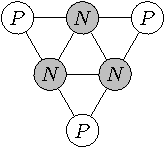
\includegraphics{diag9}
\caption{Newton diagram for
$Q(x,y,t)=x^2+y^2+t^2
- xy - yt - xt$.\label{fig:newton}}
\end{center}
\end{figure}

We will say that two points (or monomials) are \emph{adjacent}
if the corresponding monomials $m_1$ and $m_2$ if
$v_1 m_1 = v_2 m_2$, where $v_1$ is $x$, $y$, or $t$
and $v_2$ is $x$, $y$, or $t$.
Between any two points (or any two monomials)
we can define the distance
$\operatorname{dist}(m_1,m_2)$ as 1 if the corresponding
monomials are adjacent, and if they are not adjacent as the length
of the
shortest path along adjacent monomials.

The {\emph{support}} $K \subset \Z^2$ of a Newton diagram $D$ is the set
of nonzero points.  That is, $K = D^{-1}(\{ P, N \})$.
We say that the support $K$ of a Newton diagram $D$ is \emph{connected} if
any two points of $K$ are joined by a path of
adjacent points of $K$.
Let $\#(D)$ be the number of nonzero points in $D$, in other words, the
cardinality of $K$.

For a set $K \subset \Z^2$, we let $\widehat{K} \subset \Z^2$ be the smallest
simplex that contains $K$.
More precisely, $\widehat{K} \subset \Z^2$ is the
smallest
set such that $K \subset \widehat{K}$ and for some
$(j,k) \in \Z^2$
and some $m \in \N$ we have
\begin{equation}
\widehat{K} = \{(a,b) \in \Z^2 : a \geq j, \, b \geq k, \, a+b \leq m \}.
\end{equation}
When $K \subset \N_0^2$ then the diameter of $\widehat{K}$ in the distance defined above
is easily seen to be $m-j-k$.  We define the \emph{size} of $K$ as the diameter of
$\widehat{K}$ plus 1.  Therefore the size of $K$ as above is $m-j-k+1$.

\begin{prop}
$P \in \sI$ is irreducible then $D$ is connected.
\end{prop}

\begin{proof}
If $D$ is not connected, take corresponding monomials
for the two components multiply by $(x+y+t)$ and note that we
get two polynomials in $\sI$
with no monomials in common.
\end{proof}

\begin{defn}
Let $D \colon \Z^2 \to \{ 0, P, N \}$ be a Newton diagram.
Take $(j,k) \in \Z^2$
and let
\begin{equation}
E = E(j,k) \overset{\text{def}}{=} \{ (j,k) , (j-1,k) , (j,k-1) \} .
\end{equation}
We call $E$
a \emph{node} if
$D(E) \subset \{ 0, P \}$ or $D(E) \subset \{ 0, N \}$,
but $D(E) \not= \{ 0 \}$.
For a diagram $D$ let
\begin{equation}
\#(D) \overset{\text{def}}{=} \text{(number of nodes in $D$)} .
\end{equation}
\end{defn}

See \figureref{fig:newtonnodes} for an example of a diagram with nodes marked.
In dimension 2, the nodes are marked with a triangle where each vertex of the
triangle touches a point of the node.  In dimension 3 we mark the nodes
similarly with a simplex.

\begin{figure}[h!t]
\begin{center}
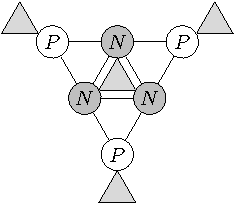
\includegraphics{diag10}
\caption{Nodes in Newton diagrams.\label{fig:newtonnodes}}
\end{center}
\end{figure}

The key point is that if the diagram of polynomial $P \in \sI$
has a node $E(j,k)$, then there must exist a term in $P$ as the only 
terms of $Q$ that can contribute to this term are those corresponding to
$E(j,k)$.

\begin{prop}\label{hj:twodim}
Let $D$ be a Newton diagram with support $K$ in two variables.
Suppose that $K$ is of size $d$,
is
connected, contains $(0,0)$. Then
\begin{equation}
\#(D) \geq \frac{d+5}{2}.
\end{equation}
\end{prop}

The proof of \propref{hj:twodim} will consist of two short lemmas.
We will say that a diagram $D^\prime$ is an \emph{extension} of $D$
if the support $K^\prime$ of $D^\prime$ contains the support $K$ of $D$
and such that $D^\prime|_K = D|_K$.

\begin{lemma}\label{hj:thm:filling}
Let $D$ and $K$ be as in \propref{hj:twodim}.  Let $m < d$ and suppose that
$K$ contains all points $(j,k)$ with $j+k \leq m-1$.  Then there exists
a Newton diagram $D'$ with support $K' \supset K$
such that $D' |_K = D$
and such that $\#(D') \leq \#(D)$ and such
that $K'$ 
contains all points $(j,k)$ with $j+k \leq m$.
\end{lemma}

\begin{proof}
We change the $0$-points at level $k$ into alternating $N$ and $P$-points, one
connected group of $0$-points of level $k$ at a time.
There must be at least one
$P$ or $N$-point at the $k$-level.  There are two cases that we should
consider.  In the first case, the group of $0$-points has $N$ or $P$-points on
both sides.  In this case no new nodes can possibly be created.

If the group goes all the way to the end of the positive quadrant, then
we have to consider the two possible alternating strings of $P$s and $N$s.
One of them will not create a new node at the point at the boundary of
the positive quadrant.
See \figureref{fig:filling}.  The circles with the dark borders
are the nonzero points that were added in a single step.
\end{proof}

\begin{figure}[h!t]
\begin{center}
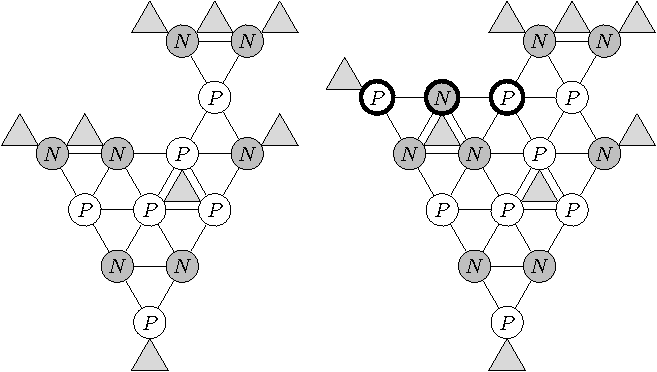
\includegraphics{diag8}
\caption{Filling a 2-dimensional diagram.\label{fig:filling}}
\end{center}
\end{figure}

By induction using
\lemmaref{hj:thm:filling} we obtain a diagram with
support
$K = \{(a,b) \in \N_0^2 \mid a+b < d\}$.
\propref{hj:twodim} now follows from the following lemma.

\begin{lemma}\label{dkr-lemma}
Let $D$ be a Newton diagram in two variables with support $K$ of size $d$
and suppose that $K$ 
contains all $(a,b) \in \N_0^2$
with $a+b < d$. Then $D$ has at least
$\frac{d+5}{2}$ nodes.
\end{lemma}

\begin{proof}
First count the number of nodes
that involve points at level $d$ (all $0$-points) or $d-1$
(no $0$-points).  The number of nodes is $d+1-k$ where $k$
is the number of sign changes at the $d-1$ level. 

Now look at two adjacent levels less than $d$.  If the number of
sign changes in one level is $m$ and the number of sign changes in
the lower level is $n$, then there
must be at least 
$\max\{ \frac{m-n}{2} , 0 \}$ nodes involving points only on these two levels.
Now by induction plus adding the node at the bottom will complete the proof.
\end{proof}

Finally we prove the following lemma that at once implies
\thmref{thm:hj:maindim2thm} as soon as we note that the number of nodes
bounds the number of terms in $P$.

\begin{lemma}
Let $D$ be a Newton diagram with connected support $K$ of size $d$
in two variables. Then
\begin{equation}
\#(D) \geq \frac{d+5}{2}.
\end{equation}
\end{lemma}

\begin{proof}
Without loss of generality we may assume
that the support $K$ contains a point 
$(a,0)$ and a point $(0,b)$ for some $a$ and $b$.  By connectedness $K$ must
contain a connected path from $(a,0)$ to $(0,b)$.
By the proof of
\lemmaref{hj:thm:filling} we can change all the $0$-points of $D$ above this
connected path into $P$ and $N$-points without increasing the number of
nodes. By rotating the diagram swapping the roles of the variables
and repeating the procedure we obtain a filled in diagram so that
we can apply
\propref{hj:twodim} to complete the proof.
\end{proof}


%%%%%%%%%%%%%%%%%%%%%%%%%%%%%%%%%%%%%%%%%%%%%%%%%%%%%%%%%%%%%%%%%%%%%%%%%%%%%%
%%%%%%%%%%%%%%%%%%%%%%%%%%%%%%%%%%%%%%%%%%%%%%%%%%%%%%%%%%%%%%%%%%%%%%%%%%%%%%
%%%%%%%%%%%%%%%%%%%%%%%%%%%%%%%%%%%%%%%%%%%%%%%%%%%%%%%%%%%%%%%%%%%%%%%%%%%%%%

%FIXME: else I don't get links, weird
%\def\MR#1{\relax\ifhmode\unskip\spacefactor3000 \space\fi%
  %\href{http://www.ams.org/mathscinet-getitem?mr=#1}{MR#1}}
\def\myDOI#1{\href{http://dx.doi.org/#1}{#1}}



%FIXME
%\cleardoublepage  
\clearpage
\phantomsection
\addcontentsline{toc}{chapter}{Further Reading}
\markboth{FURTHER READING}{FURTHER READING}
\begin{bibchapter}[Further Reading]

Here are useful books for extra reading, some were cited.
Papers cited appear in the next section.

\begin{biblist}[\normalsize]

\bib{AG:linop}{book}{
   author={Akhiezer, N. I.},
   author={Glazman, I. M.},
   title={Theory of linear operators in Hilbert space},
   %note={Translated from the Russian and with a preface by Merlynd Nestell;
   %Reprint of the 1961 and 1963 translations;
   %Two volumes bound as one},
   publisher={Dover Publications Inc.},
   place={New York},
   date={1993},
   pages={xiv+147+iv+218},
   isbn={0-486-67748-6},
   review={\MR{1255973}},
   %review={\MR{1255973 (94i:47001)}},
}


\bib{BER:book}{book}{
   author={Baouendi, M. Salah},
   author={Ebenfelt, Peter},
   author={Rothschild, Linda Preiss},
   title={Real submanifolds in complex space and their mappings},
   series={Princeton Mathematical Series},
   volume={47},
   publisher={Princeton University Press},
   place={Princeton, NJ},
   date={1999},
   pages={xii+404},
   isbn={0-691-00498-6},
   review={\MR{1668103}},
   %review={\MR{1668103 (2000b:32066)}},
}


\bib{Boggess}{book}{
   author={Boggess, Albert},
   title={CR manifolds and the tangential Cauchy-Riemann complex},
   series={Studies in Advanced Mathematics},
   publisher={CRC Press},
   place={Boca Raton, FL},
   date={1991},
   pages={xviii+364},
   isbn={0-8493-7152-X},
   review={\MR{1211412}},
   %review={\MR{1211412 (94e:32035)}},
}

\bib{Chirka}{book}{
   author={Chirka, E. M.},
   title={Complex analytic sets},
   series={Mathematics and its Applications (Soviet Series)},
   volume={46},
   %note={Translated from the Russian by R. A. M. Hoksbergen},
   publisher={Kluwer Academic Publishers Group},
   place={Dordrecht},
   date={1989},
   pages={xx+372},
   isbn={0-7923-0234-6},
   review={\MR{1111477}},
   %review={\MR{1111477 (92b:32016)}},
}





\bib{DAngelo}{book}{
   author={D'Angelo, John P.},
   title={Several complex variables and the geometry of real hypersurfaces},
   series={Studies in Advanced Mathematics},
   publisher={CRC Press},
   place={Boca Raton, FL},
   date={1993},
   pages={xiv+272},
   isbn={0-8493-8272-6},
   review={\MR{1224231}},
   %review={\MR{1224231 (94i:32022)}},
}

\bib{Hormander}{book}{
   author={H{\"o}rmander, Lars},
   title={An introduction to complex analysis in several variables},
   series={North-Holland Mathematical Library},
   volume={7},
   edition={3},
   publisher={North-Holland Publishing Co.},
   place={Amsterdam},
   date={1990},
   pages={xii+254},
   isbn={0-444-88446-7},
   review={\MR{1045639}},
   %review={\MR{1045639 (91a:32001)}},
}

\bib{HornJohnson}{book}{
   author={Horn, Roger A.},
   author={Johnson, Charles R.},
   title={Matrix analysis},
   publisher={Cambridge University Press},
   place={Cambridge},
   date={1985},
   pages={xiii+561},
   isbn={0-521-30586-1},
   review={\MR{832183}},
   %review={\MR{832183 (87e:15001)}},
}

\bib{Krantz}{book}{
   author={Krantz, Steven G.},
   title={Function theory of several complex variables},
   series={The Wadsworth \& Brooks/Cole Mathematics Series},
   edition={2},
   publisher={Wadsworth \& Brooks/Cole Advanced Books \& Software},
   place={Pacific Grove, CA},
   date={1992},
   pages={xvi+557},
   isbn={0-534-17088-9},
   review={\MR{1162310}},
   %review={\MR{1162310 (93c:32001)}},
}


\bib{Rudin:fanal}{book}{
   author={Rudin, Walter},
   title={Functional analysis},
   series={International Series in Pure and Applied Mathematics},
   edition={2},
   publisher={McGraw-Hill Inc.},
   place={New York},
   date={1991},
   pages={xviii+424},
   isbn={0-07-054236-8},
   review={\MR{1157815}},
   %review={\MR{1157815 (92k:46001)}},
}

\bib{Rudin:ball}{book}{
   author={Rudin, Walter},
   title={Function theory in the unit ball of ${\bf C}^{n}$},
   series={Grundlehren der Mathematischen Wissenschaften [Fundamental
   Principles of Mathematical Science]},
   volume={241},
   publisher={Springer-Verlag},
   place={New York},
   date={1980},
   pages={xiii+436},
   isbn={0-387-90514-6},
   review={\MR{601594}},
   %review={\MR{601594 (82i:32002)}},
}




\bib{Whitney}{book}{
   author={Whitney, Hassler},
   title={Complex analytic varieties},
   publisher={Addison-Wesley Publishing Co., Reading, Mass.-London-Don
   Mills, Ont.},
   date={1972},
   pages={xii+399},
   review={\MR{0387634}},
   %review={\MR{0387634 (52 \#8473)}},
}

\end{biblist}
\end{bibchapter}

%%%%%%%%%%%%%%%%%%%%%%%%%%%%%%%%%%%%%%%%%%%%%%%%%%%%%%%%%%%%%%%%%%%%%%%%%%%%%%

%\cleardoublepage  
%\phantomsection
\addcontentsline{toc}{chapter}{Bibliography}
\markboth{BIBLIOGRAPHY}{BIBLIOGRAPHY}
\begin{bibchapter}[Bibliography]
\begin{biblist}[\normalsize]

\bib{CS83}{article}{
   author={Cima, J.\ A.},
   author={Suffridge, T.\ J.},
   title={A reflection principle with applications to proper holomorphic
   mappings},
   journal={Math.\ Ann.},
   volume={265},
   date={1983},
   number={4},
   pages={489--500},
   issn={0025-5831},
   %review={\MR{721883 (84m:32033)}},
   review={\MR{721883}},
   doi={\myDOI{10.1007/BF01455949}},
}


\bib{DKR}{article}{
   author={D'Angelo, John P.},
   author={Kos, {\v{S}}imon},
   author={Riehl, Emily},
   title={A sharp bound for the degree of proper monomial mappings between
   balls},
   journal={J.\ Geom.\ Anal.},
   volume={13},
   date={2003},
   number={4},
   pages={581--593},
   issn={1050-6926},
   doi={\myDOI{10.1007/BF02921879}},
   %review={\MR{2005154 (2004i:32028)}},
   review={\MR{2005154}},
}

\bib{DF}{article}{
   author={Diederich, Klas},
   author={Fornaess, John E.},
   title={Pseudoconvex domains with real-analytic boundary},
   journal={Ann.\ Math.\ (2)},
   volume={107},
   date={1978},
   number={2},
   pages={371--384},
   %review={\MR{0477153 (57 \#16696)}},
   review={\MR{0477153}},
}



\bib{Dor}{article}{
   author={Dor, Avner},
   title={Proper holomorphic maps between balls in one co-dimension},
   journal={Ark.\ Mat.},
   volume={28},
   date={1990},
   number={1},
   pages={49--100},
   issn={0004-2080},
   review={\MR{1049642}},
   doi={\myDOI{10.1007/BF02387366}},
}

\bib{FaranB2B3}{article}{
   author={Faran, James J.},
   title={Maps from the two-ball to the three-ball},
   journal={Invent.\ Math.},
   volume={68},
   date={1982},
   number={3},
   pages={441--475},
   issn={0020-9910},
   %review={\MR{669425 (83k:32038)}},
   review={\MR{669425}},
   doi={\myDOI{10.1007/BF01389412}},
}

\bib{Faran86}{article}{
   author={Faran, James J.},
   title={The linearity of proper holomorphic maps between balls in the low
   codimension case},
   journal={J.\ Differential Geom.},
   volume={24},
   date={1986},
   number={1},
   pages={15--17},
   issn={0022-040X},
   %review={\MR{857373 (87k:32050)}},
   review={\MR{857373}},
}



\bib{Forstneric89}{article}{
   author={Forstneri{\v{c}}, Franc},
   title={Extending proper holomorphic mappings of positive codimension},
   journal={Invent.\ Math.},
   volume={95},
   date={1989},
   number={1},
   pages={31--61},
   issn={0020-9910},
   %review={\MR{969413 (89j:32033)}},
   review={\MR{969413}},
   doi={\myDOI{10.1007/BF01394144}},
}

\bib{Hamada}{article}{
   author={Hamada, Hidetaka},
   title={Rational proper holomorphic maps from ${\mathbf B}^n$ into
   ${\mathbf B}^{2n}$},
   journal={Math.\ Ann.},
   volume={331},
   date={2005},
   number={3},
   pages={693--711},
   issn={0025-5831},
   %review={\MR{2122546 (2005k:32020)}},
   review={\MR{2122546}},
   doi={\myDOI{10.1007/s00208-004-0606-2}},
}



\bib{HornSergeichuk}{article}{
   author={Horn, Roger A.},
   author={Sergeichuk, Vladimir V.},
   title={Canonical forms for complex matrix congruence and *congruence},
   journal={Linear Algebra Appl.},
   volume={416},
   date={2006},
   number={2-3},
   pages={1010--1032},
   issn={0024-3795},
   review={\MR{2242477}},
   doi={\myDOI{10.1016/j.laa.2006.01.005}},
}

\bib{Huang99}{article}{
   author={Huang, Xiaojun},
   title={On a linearity problem for proper holomorphic maps between balls
   in complex spaces of different dimensions},
   journal={J.\ Differential Geom.},
   volume={51},
   date={1999},
   number={1},
   pages={13--33},
   issn={0022-040X},
   %review={\MR{1703603 (2000e:32020)}},
   review={\MR{1703603}},
}

\bib{HJ01}{article}{
   author={Huang, Xiaojun},
   author={Ji, Shanyu},
   title={Mapping ${\mathbf B}^n$ into ${\mathbf B}^{2n-1}$},
   journal={Invent.\ Math.},
   volume={145},
   date={2001},
   number={2},
   pages={219--250},
   issn={0020-9910},
   %review={\MR{1872546 (2002i:32013)}},
   review={\MR{1872546}},
   doi={\myDOI{10.1007/s002220100140}},
}


\bib{HJX}{article}{
   author={Huang, Xiaojun},
   author={Ji, Shanyu},
   author={Xu, Dekang},
   title={A new gap phenomenon for proper holomorphic mappings from $B^n$
   into $B^N$},
   journal={Math.\ Res.\ Lett.},
   volume={13},
   date={2006},
   number={4},
   pages={515--529},
   issn={1073-2780},
   review={\MR{2250487}},
}


\bib{LancasterRodman}{article}{
   author={Lancaster, Peter},
   author={Rodman, Leiba},
   title={Canonical forms for Hermitian matrix pairs under strict
   equivalence and congruence},
   journal={SIAM Rev.},
   volume={47},
   date={2005},
   number={3},
   pages={407--443},
   issn={0036-1445},
   review={\MR{2178635}},
   doi={\myDOI{10.1137/S003614450444556X}},
}

\bib{LP}{article}{
   author={Lebl, Ji\v{r}\'i},
   author={Peters, Han},
   title={Polynomials constant on a hyperplane and CR maps of hyperquadrics},
   note = {\href{http://www.arxiv.org/abs/0910.2673}{arXiv:0910.2673}},
   journal={Mosc.\ Math.\ J.},
   volume={11},
   year={2011},
   number={2},
   pages={287--317},
   review={\MR{2859238}},
}

\bib{Webster79}{article}{
   author={Webster, S.\ M.},
   title={On mapping an $n$-ball into an $(n+1)$-ball in complex spaces},
   journal={Pacific J.\ Math.},
   volume={81},
   date={1979},
   number={1},
   pages={267--272},
   issn={0030-8730},
   %review={\MR{543749 (81h:32022)}},
   review={\MR{543749}},
}


\end{biblist}
\end{bibchapter}

%%%%%%%%%%%%%%%%%%%%%%%%%%%%%%%%%%%%%%%%%%%%%%%%%%%%%%%%%%%%%%%%%%%%%%%%%%%%%%
%%%%%%%%%%%%%%%%%%%%%%%%%%%%%%%%%%%%%%%%%%%%%%%%%%%%%%%%%%%%%%%%%%%%%%%%%%%%%%
%%%%%%%%%%%%%%%%%%%%%%%%%%%%%%%%%%%%%%%%%%%%%%%%%%%%%%%%%%%%%%%%%%%%%%%%%%%%%%

%\cleardoublepage  
\clearpage  
\phantomsection
\addcontentsline{toc}{chapter}{\indexname}  
\printindex

\end{document}
